\chapter{Search for invisibly decaying Higgs bosons in Run 1 parked data}
\label{chap:parked}
The parked data, described in \SectionRef{sec:triggers}, used for this analysis was collected using a range of triggers with similar but looser requirements than that used for the prompt data analysis described in the previous chapter. These looser requirements allow areas of phase space which were previously removed by the prompt trigger to be used. However, these areas also have very high levels of \ac{QCD} multijet backgrounds, and require the analysis selection 
and some background estimation methods to be redesigned compared to the prompt analysis.

%??CHECK PLOT AXIS LABEL SIZES AND THAT LEGEND TERMS ARE STANDARD OR IN TEXT

%??parkedgains111114.pdf for parked vs prompt limits
%??closure161214update for closure test
%??invupdate081214.pdf for some pileup studies
%??framework synch fwprogress300614.pdf
%??preapproval for source of gain and other good things
%??As above for prompt data analysis but focus on differences and limit setting:
%??systematic improvements, signal region optimisation, differences in background estimations including options not used
%??lepton and jet pt requirements
\section{Trigger}
\label{sec:parkedtrigger}
The parked data trigger varied throughout LHC Run 1 due to the estimates of both the trigger bandwidth available and the rate of the triggers used in the particular LHC conditions that occurred being updated. Run 1 was split into 4 ``eras'', A, B, C and D. During era A data was not being parked, so the prompt data is used. The two other triggers used, one for eras B and C, and one for era D, differed from the prompt trigger in that there was no requirement on the \MET present at \ac{HLT} level in each event and the jet \pt and \Mjj requirements were looser. These looser requirements allow the trigger driven selection applied in the prompt data analysis to be relaxed, and more optimal signal and background control regions to be used. As the region accessible with the parked data includes the prompt data signal region as a subset, no improvement would be possible from applying the analysis designed for the prompt data to the parked data without modification. The exact values of the trigger selection cuts are summarised in \TableRef{tab:parkedtrig}.

\begin{table}
  \caption{A summary of the requirements of the triggers used for this analysis in each of LHC Run 1's eras. For the jet requirements all triggers require that there is at least one pair of jets in the event satisfying all of the jet requirements listed in this table. All requirements are on \ac{HLT} variables unless stated otherwise.}
  \label{tab:parkedtrig}
  \begin{tabular}{lc|c|c}
    \hline\hline
    \multirow{2}{*}{Variable} & \multicolumn{3}{c}{Cut in era} \\
    \cline{2-4}
    & A & B \& C & D \\
    \hhline{====}
    L1 \MET & \multicolumn{3}{c}{$>40$ \GeV} \\
    \hline
    \METnoMU & $>65$ \GeV & \multicolumn{2}{c}{No requirement} \\
    \hline
    jet \pt of both jets & $>40$ \GeV & $>35$ \GeV & $>30$ \GeV \\
    \hline
    \Mjj & $>800$ \GeV & \multicolumn{2}{c}{$>700$ \GeV} \\
    \hline
    \detajj & \multicolumn{3}{c}{$>3.5$} \\
    \hline
    $\eta_{j1}\cdot\eta_{j2}$ & \multicolumn{3}{c}{$>0$} \\
    \hline
    \hline
  \end{tabular}
\end{table}

In order to get the biggest improvement in sensitivity from the parked data, it is important to measure the trigger efficiency accurately, so as to take advantage of as much of the increase in accessible phase space as possible. As three different triggers are used the measurement of trigger efficiency must be performed separately for each one. Also, the variables used in the trigger are highly correlated with each other. These correlations mean it is important to either only use regions of phase space where the trigger is fully efficient, as was done in the prompt analysis, or to measure the trigger efficiency in a way that accurately models the effect of these correlations. The cuts required to ensure that each trigger is fully efficient throughout the region selected can be ascertained from \FigureRef{fig:prompttrigplots}.

As the trigger used in era A was the same as that used for the prompt analysis, no relaxation would be possible if full trigger efficiency is required and the data from era A is to be used. Era A only accounts for 5\% of the total data, so one possibility is not to use the era A data and to relax the selection to the point of full efficiency of the next tightest trigger. However, it would still be necessary to discard data in the trigger turn on region which is expected to contain signal events. For these reasons several approaches to measuring the trigger efficiency as a function of the values of all variables used in it were investigated.

First, the trigger efficiency was measured three dimensionally as a function of \METnoMU, \Mjj and sub-leading jet's \pt. An example of one of the results of these measurements in one of the bins in \METnoMU for the era B and C, and the era D triggers can be seen in \FigureRef{fig:parked3dtrigeff}. The three variables used were chosen because the trigger becomes fully efficient very quickly as a function of the $\eta$ related variables, so no parameterisation of this efficiency is necessary. The number and size of the bins was chosen to ensure that sufficient events are present in each bin to prevent the statistical error on the efficiency measurement being larger than the differences between bins. As can be seen from the figure, this leads to very large differences in efficiency between bins, which leads to discontinuities in the \METnoMU, \Mjj and sub-leading jet \pt distributions when the measured efficiency was applied to \ac{MC} events as a weight. This method was therefore not suitable for use in the final analysis.
%trigeff070414.pdf for full 3D binned plot
\begin{figure} 
  \subfloat[]{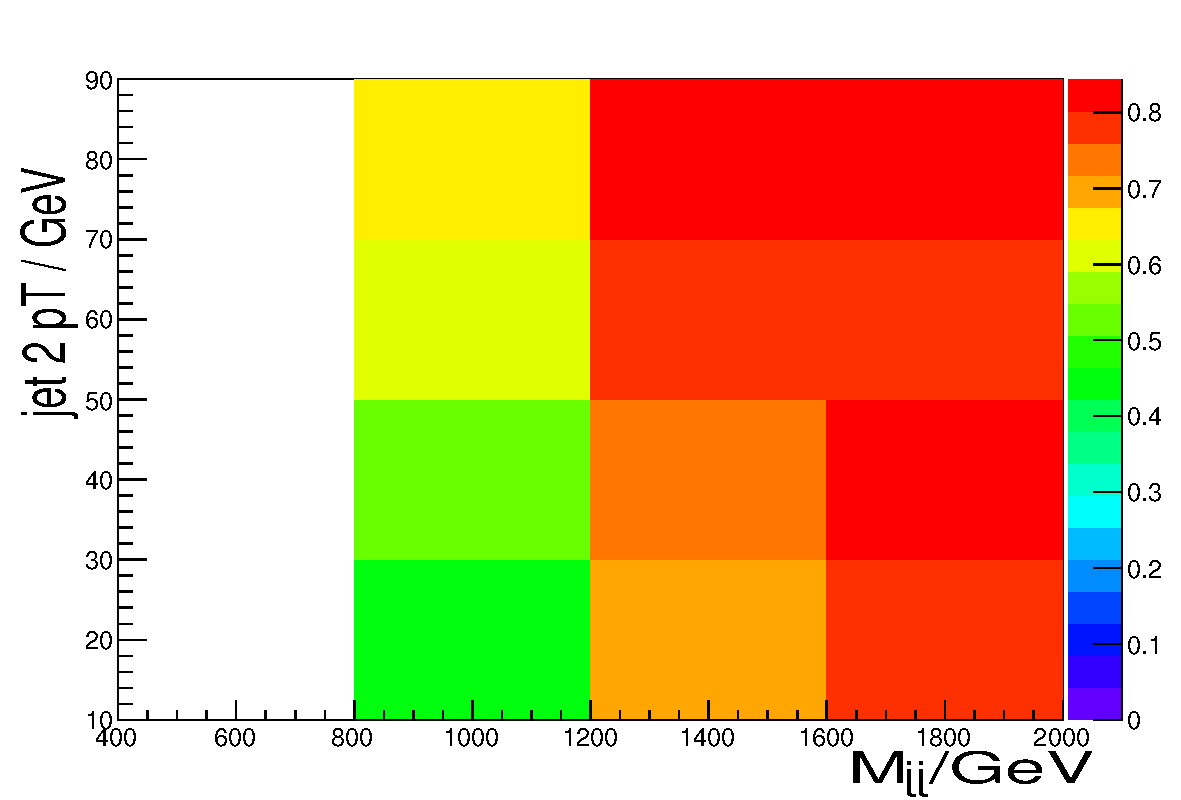
\includegraphics[width=.6\largefigwidth]{plots/parked/HLT_DiJet35_MJJ700_AllJets_DEta3p5_VBFmet120trigeff.pdf}}
  \subfloat[]{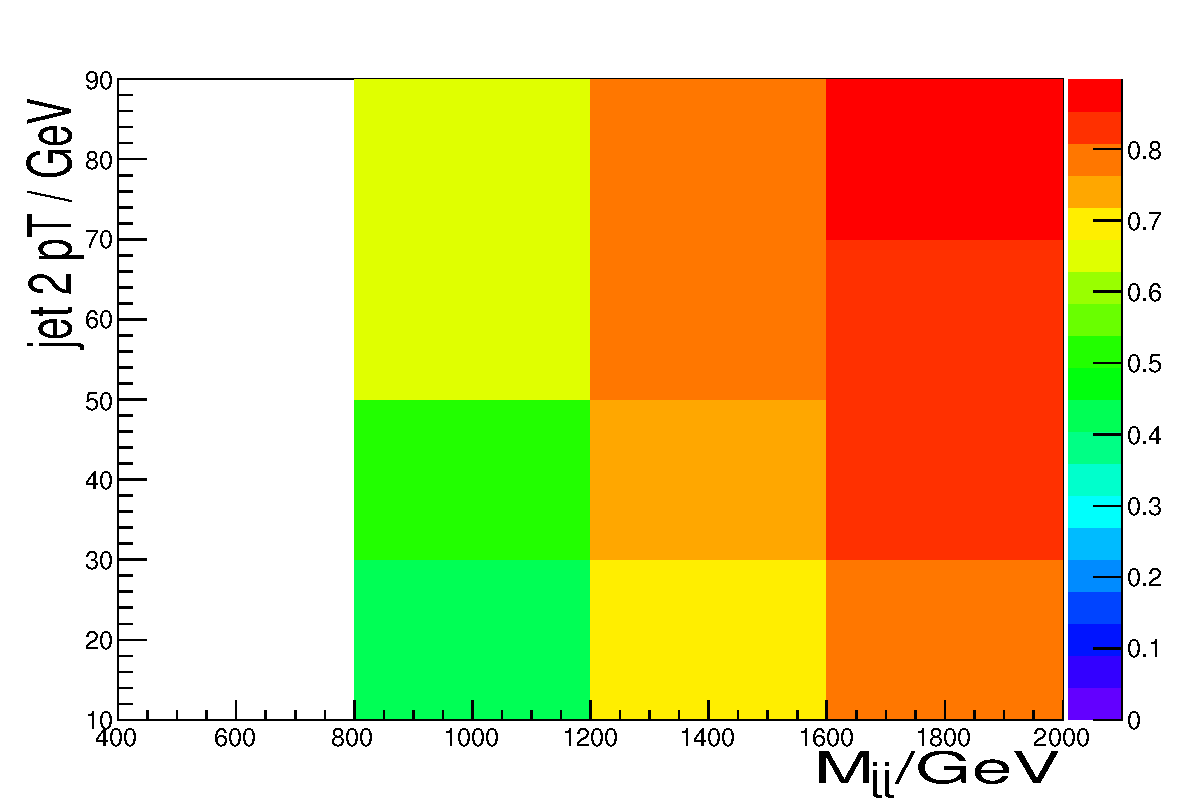
\includegraphics[width=.6\largefigwidth]{plots/parked/HLT_DiJet30_MJJ700_AllJets_DEta3p5_VBFmet120trigeff.pdf}}
 \caption{The efficiency for the trigger (color-scale) used in eras B and C (a) and era D (b), as a function of \Mjj and sub-leading jet \pt for events with \METnoMU between 60 and 120 \GeV. The efficiency was measured using a single muon dataset collected with an orthogonal trigger.}
  \label{fig:parked3dtrigeff}
\end{figure}

In order to achieve a smoother trigger efficiency parameterisation, coarse bins in \Mjj and sub-leading jet \pt were chosen and a fit to the \METnoMU efficiency distribution in each bin was performed, using the following function:
\begin{equation}
  \label{eq:parkedtrigfunc}
  f\left(x\right)=\frac{A}{2}\cdot\left(1+ \frac{2}{\sqrt{\pi}}\int_{0}^{\frac{x-B}{\sqrt{C}}}e^{-t^{2}}\mathrm{d}t\right),
\end{equation}
which has a maximum value of A, and is derived from the error function with centre B and width C. The width, maximum and centre of the function are all allowed to float in the fit. The events used in this study were required to have leading jet \pt$>50$ \GeV, $\eta_{j1}\cdot\eta_{j2}<0$ and \detajj$>3.6$ to ensure that there are no inefficiencies due to these variables. The results of these fits for the two \Mjj and sub-leading jet \pt bins containing the most events entering the final analysis selection are shown in \FigureRef{fig:parkedtrigeff}, and the results for the remaining bins are shown in \AppendixRef{app:trigeffs}. Some of the plots in the appendix indicate that the parameters of the fit have taken extreme values, or have very large uncertainties. These extreme values and poor fits are mostly due to low numbers of events in the bin. The analysis selection described in \SectionRef{sec:parkedsel}, ensures that no events in these bins are used in the analysis.

\begin{figure}
  \subfloat[]{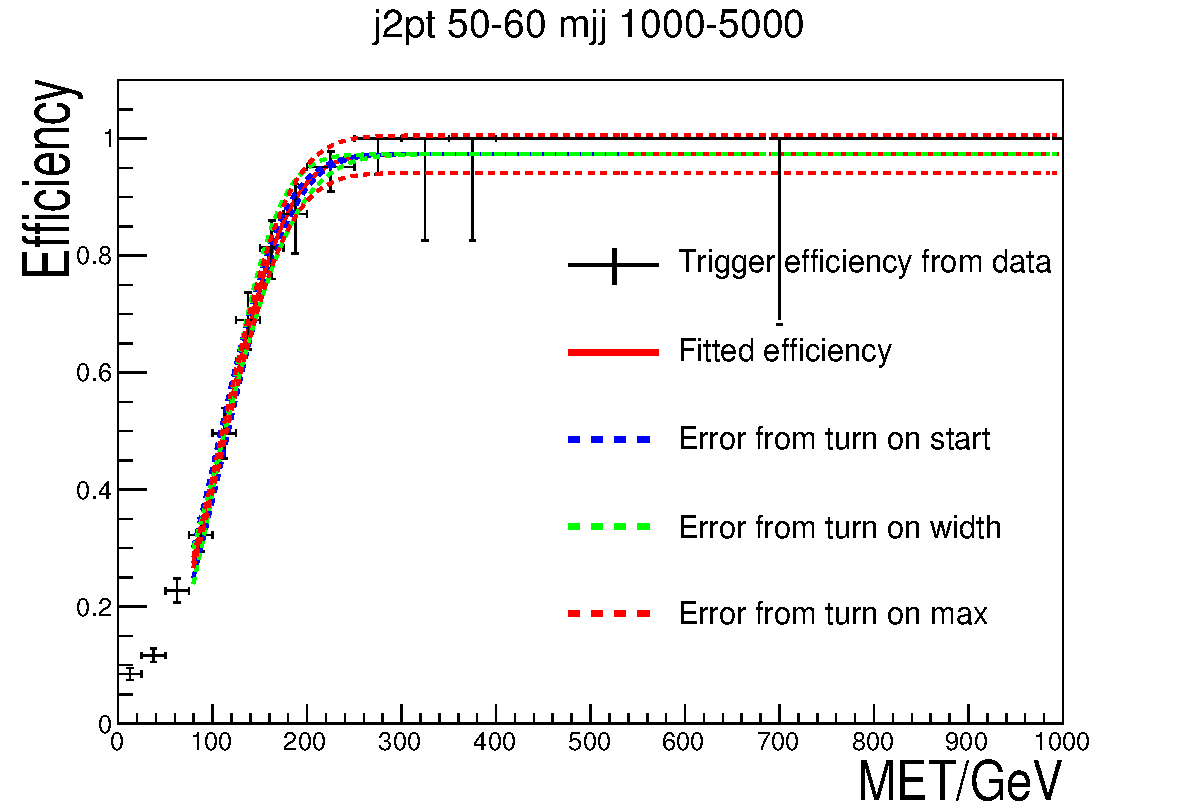
\includegraphics[width=.6\largefigwidth]{plots/parked/trigfitplots/hData_MET_1D_35D.pdf}}
  \subfloat[]{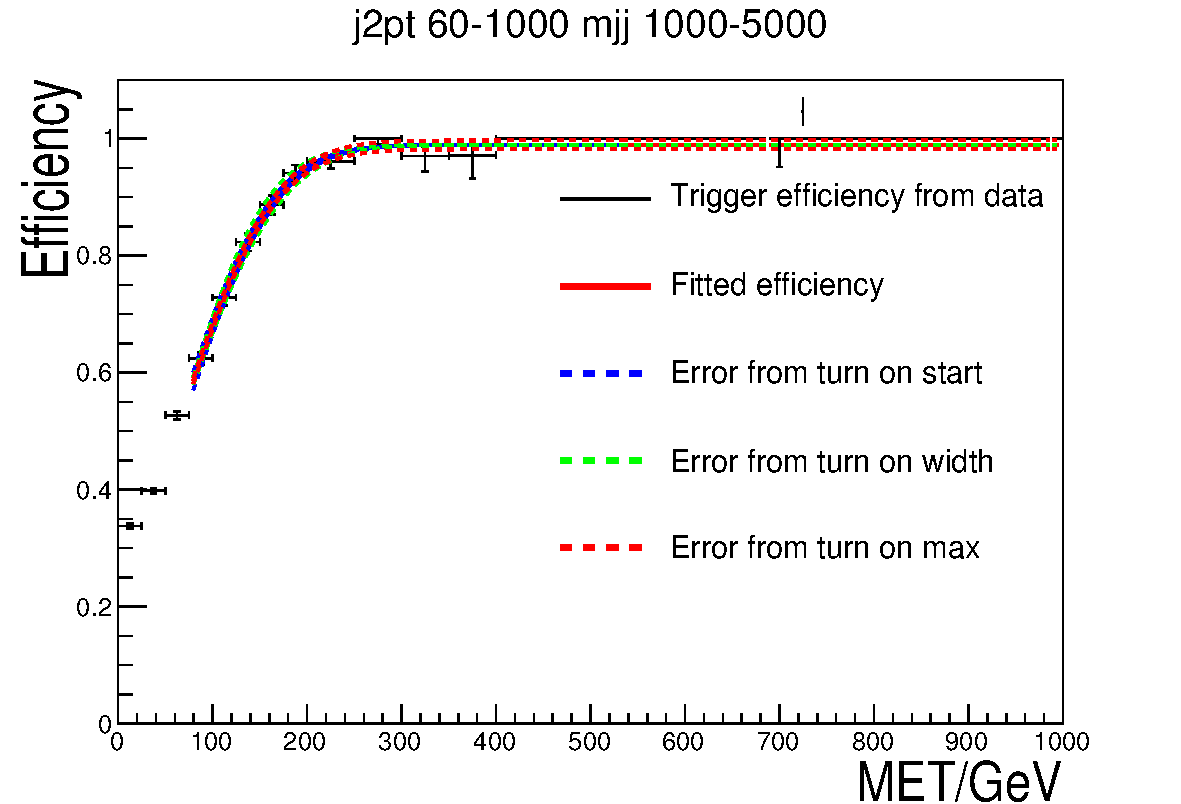
\includegraphics[width=.6\largefigwidth]{plots/parked/trigfitplots/hData_MET_1D_45D.pdf}}
  \caption{The results of performing a fit of the function in \EquationRef{eq:parkedtrigfunc} to the efficiency of the trigger used in era D, measured in a sample of single muon events collected with an orthogonal trigger. The dashed bands show the uncertainty on the fit due to each of the three parameters of the fit. The two bins of dijet mass (mjj) and sub-leading jet's \pt (j2pt) shown are those with the two highest numbers of events from the final signal region described in \SectionRef{sec:parkedsel}.}
  \label{fig:parkedtrigeff}
\end{figure}

Each \ac{MC} event was weighted by the average of the efficiency found for each of the three triggers weighted by the amount of integrated luminosity recorded using each trigger as shown in the following equation:
\begin{equation}
  \label{eq:parkedtrigweight}
  w\left(p_{\mathrm{T}j2},\Mjj,\METnoMU\right)=\frac{\sum_{i}\mathcal{L}_{i}\epsilon_{i}\left(p_{\mathrm{T}j2},\Mjj,\METnoMU\right)}{\sum_{i}\mathcal{L}_{i}},
\end{equation}
Where $i$ are the three triggers, $\epsilon_{i}\left(p_{\mathrm{T}j2},\Mjj,\METnoMU\right)$ is the measured efficiency for trigger $i$ as a function of the event's sub-leading jet \pt, \Mjj and \METnoMU, and $\mathcal{L}_{i}$ is the integrated luminosity collected using trigger $i$. The resulting trigger efficiency varies smoothly and leads to no unphysical discontinuities in the distributions of event variables as can be seen from the figures in the remainder of this chapter.

\section{Event selection}
\label{sec:parkedsel}
As mentioned above a significant challenge of the parked data analysis is that the areas of phase space collected by the parked data triggers but not by the prompt data triggers have very large contributions from \ac{QCD} multijet backgrounds. The \ac{QCD} multijet contribution to \ac{VBF} analyses is very hard to model because whilst the cross-sections for these processes are very high, the probability of any individual event being \ac{VBF}-like is very low. The number of \ac{MC} events that must be generated to make a representative sample is therefore prohibitively large. As a result of these difficulties, the parked data selection is separated into two stages. The first ``preselection'' stage selects a region of phase space which is not expected to be dominated by \ac{QCD} processes. After this preselection has been made the background processes expected to make contributions are the same as in the prompt data analysis, and studies were undertaken into which background estimation methods and final signal region selection led to the best expected limit.

%runcbug101114.pdf sig reg optimisation

\subsection{Preselection}
\label{sec:parkedpresel}
The first element of the preselection was motivated by the trigger. The following selection was applied to ensure that the values of all event variables are above the trigger thresholds of all triggers used:
\begin{align}
  \label{eq:parkedprepresel}
  \begin{split}
  \eta_{j1}\cdot\eta_{j2}<0,\,\mathrm{leading\,jet\,}\pt>50 \GeV, \detajj>3.6, \\
  \mathrm{subleading\,jet\,}\pt>40 \GeV, \Mjj>800 GeV, \METnoMU>90\GeV.
  \end{split}
\end{align}
Where $j1$ and $j2$ are the leading and sub-leading \pt jets in the event and are chosen as the \ac{VBF} tag jets. We also require that for the ``signal-like'' selection there are no veto electrons or muons in the event. The W+jets and Z+jets control regions used in the background estimation methods described in \SectionRef{sec:parkedbkg} impose different lepton requirements. QCD multijet processes still dominate the region defined by this selection, as can be seen in \FigureRef{fig:parkedpresel}a, where there are a lot more data events than expected from the background \ac{MC} prediction. This difference is due to mismeasured \ac{QCD} multijets events not being adequately modelled by the available \ac{MC} samples, which are described in further detail in \SectionRef{sec:parkedQCD}. The first variable that was used to achieve this reduction is the \MET significance, \METsig, which is defined as the ratio between \METnoMU and the square root of the sum of the transverse energy of all particles in the event which is an estimate of the statistical error on the \MET. The intention of the \METsig cut is to remove events which have a large amount of \MET, but also have an even larger amount of visible energy, meaning that the \MET is likely to be from mismeasurement of the visible particles. The preselection requires that this variable be greater than 3. The value of this cut was chosen by looking at \FigureRef{fig:parkedpresel}a and removing the region with the most disagreement between data and \ac{MC}. The resulting region shown in \FigureRef{fig:parkedpresel}b still does not display good agreement between data and the \ac{MC} prediction, however the disagreement is smaller.

After the cut on \METsig, a requirement that the \METnoMU is not too close to any jets in \phi was made. This requirement was motivated by the high probability for the \MET to be aligned with a jet in the case where the jet has been mismeasured. Two variables were investigated, the first was the minimum azimuthal angle difference between either of the two tag jets and the \METnoMU, \jetmetdphileading, and the second was the minimum azimuthal angle difference between any jet with \pt greater than 30 \GeV and the \METnoMU, \jetmetdphi. At a similar signal efficiency the difference between the observed number of events and the \ac{MC} background prediction, which is an indication of the remaining \ac{QCD} multijet background, was found to be 80\% smaller for a cut on \jetmetdphi than a cut on \jetmetdphileading. The same cut on \jetmetdphi was also found to reduce top quark related backgrounds by a factor of two compared to a cut on \jetmetdphileading. We therefore require that \jetmetdphi$>1.0$ for events to pass the preselection. \jetmetdphi was found to give significantly better signal efficiency than \dphijj for the same background rejection, so no cut was made on \dphijj.

%AN-14-243
\begin{figure}
  \subfloat[]{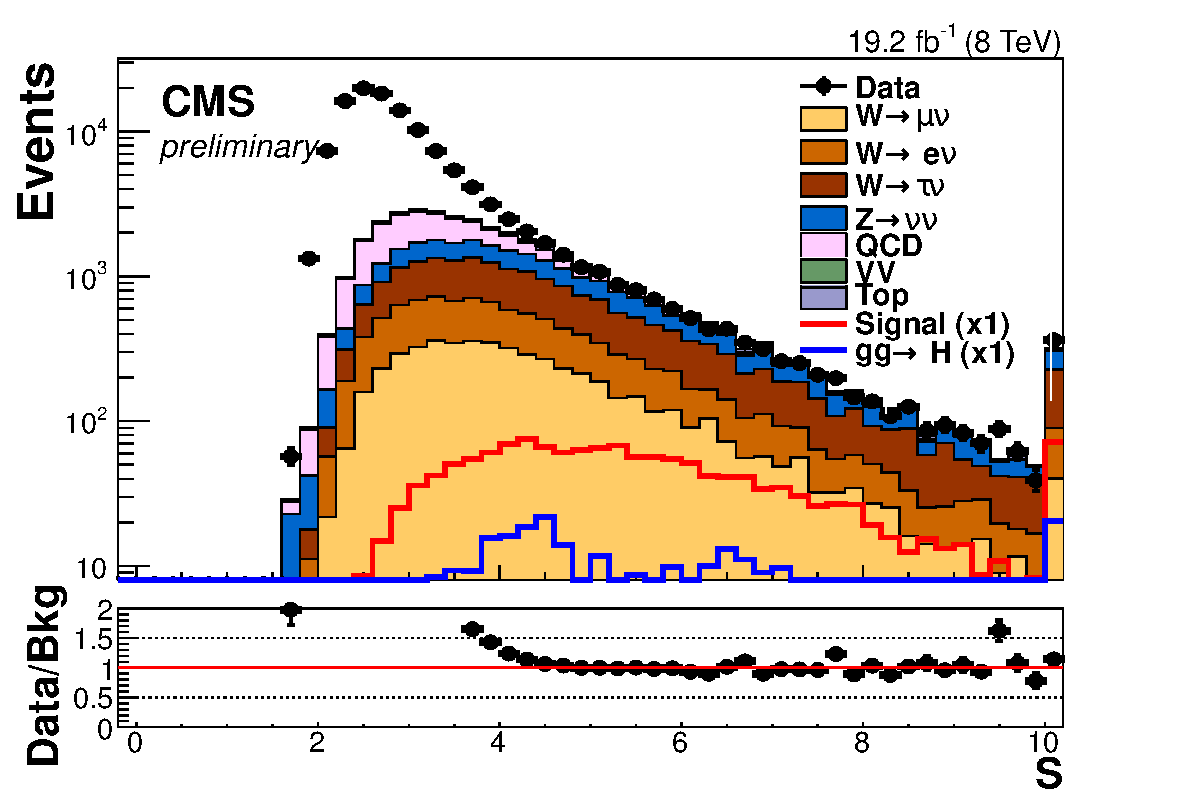
\includegraphics[width=.6\largefigwidth]{plots/parked/AN-14-243-figs/lognopreselnunu_metnomu_significance.pdf}}
  \subfloat[]{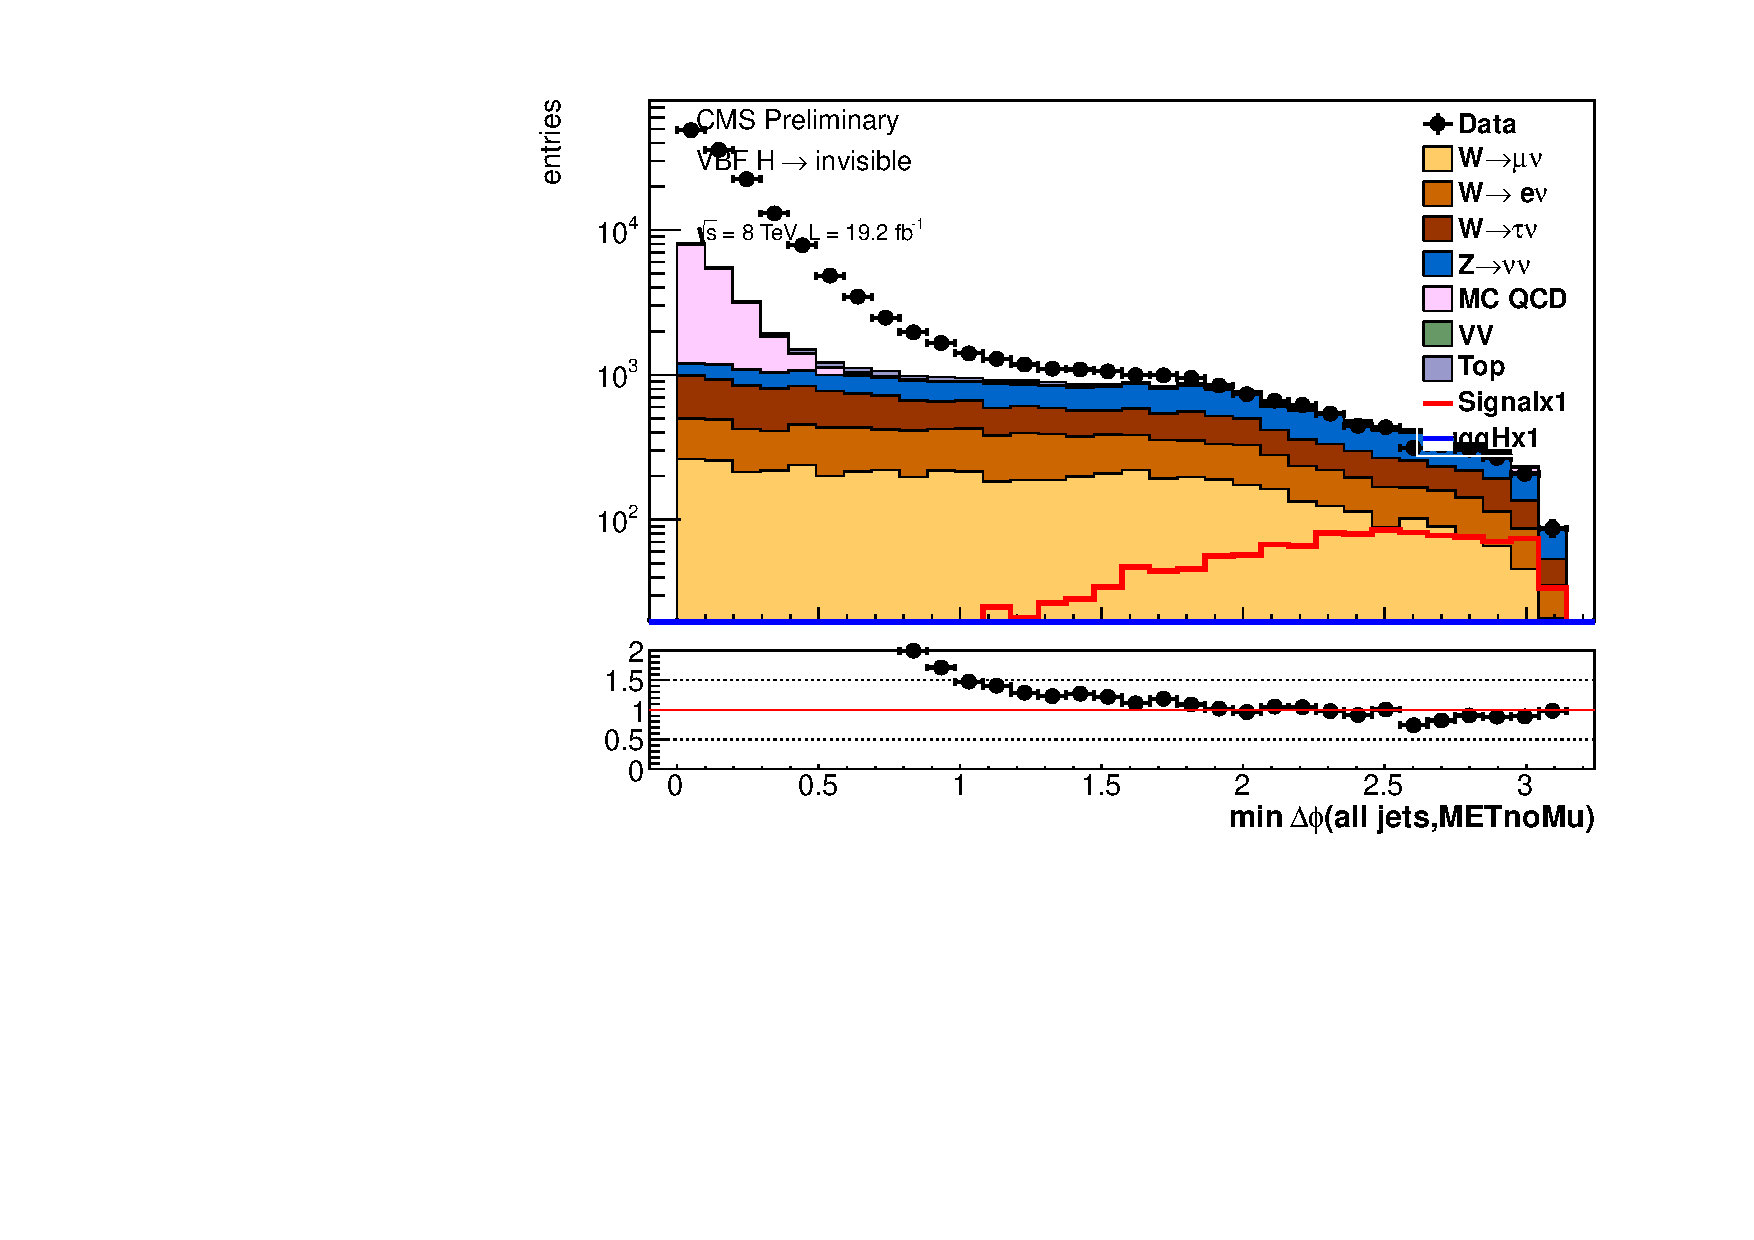
\includegraphics[width=.6\largefigwidth]{plots/parked/AN-14-243-figs/logmetsigpreselnunu_alljetsmetnomu_mindphi.pdf}}

  \subfloat[]{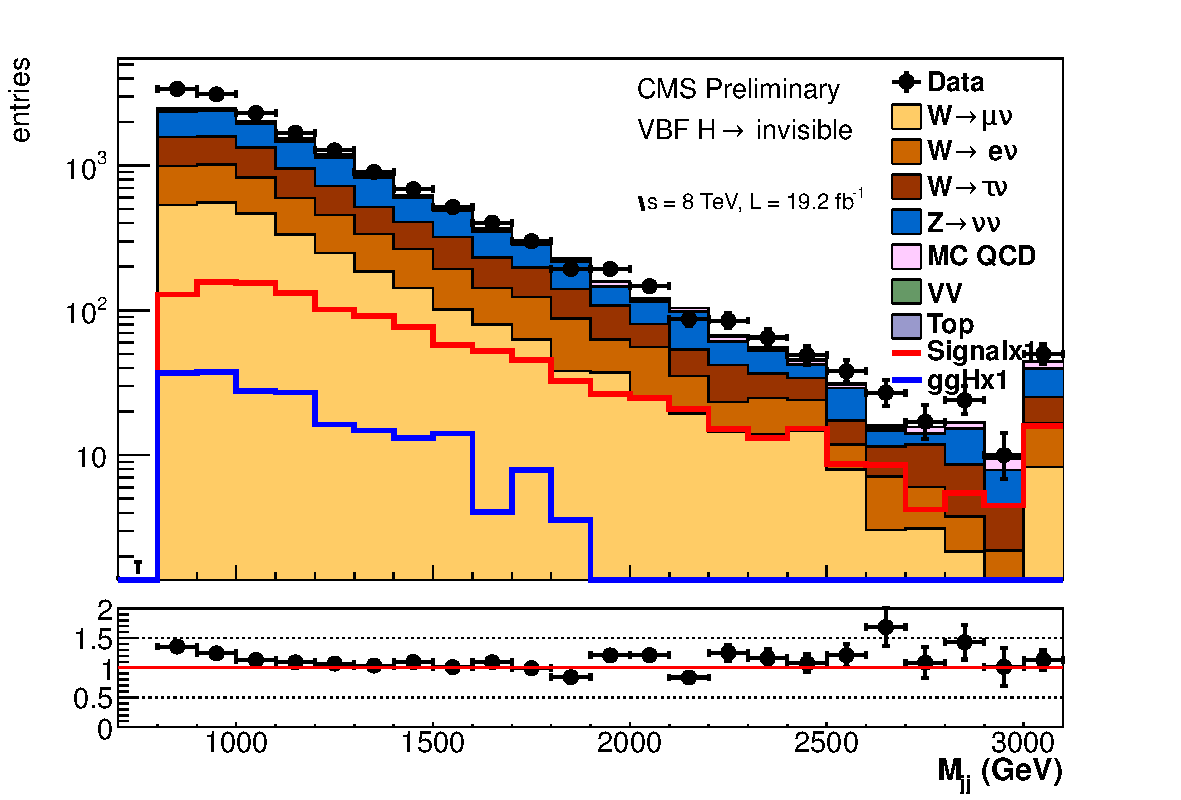
\includegraphics[width=.6\largefigwidth]{plots/parked/AN-14-243-figs/logmjj800nunu_dijet_M.pdf}}
  \caption{(a) \METsig after the trigger driven selection described in \EquationRef{eq:parkedprepresel}. (b) \jetmetdphi after the trigger driven selection and requiring \METsig$>3$. (c) \Mjj after the trigger driven selection and requiring \METsig$>3$ and \jetmetdphi$>1$. All three plots are of the signal-like region with the \ac{MC} scaled using the background estimation methods described in \SectionRef{sec:parkedbkg}. The disagreement between data and the predictions from background \ac{MC} samples is believed to be due to mismeasured \ac{QCD} multijet events which are not well modelled by the available \ac{MC} samples.}
  \label{fig:parkedpresel}
\end{figure}

%contplotsandpresel160914
The \Mjj distribution after the \jetmetdphi cut is shown in \FigureRef{fig:parkedpresel}c. Whilst the agreement for large \Mjj is good, it can be seen that the first bin of the distribution, where mismeasured \ac{QCD} multijet events would be expected, due to their not recoiling against another object, shows a significant disagreement. The final cut of the preselection is therefore to require that \Mjj$>1000$ \GeV. This cut also ensures that none of the bins of the trigger efficiency which have extreme values due to low numbers of events are used. In summary the full preselection is as follows:
\begin{equation}
  \label{eq:presel}
  \begin{split}
  \eta_{j1}\cdot\eta_{j2}<0,\,\mathrm{leading\,jet\,}\pt>50 \GeV, \detajj>3.6, \\
  \mathrm{subleading\,jet\,}\pt>40 \GeV, \Mjj>1000 GeV, \METnoMU>90\GeV, \\
  \jetmetdphi>1.0, \METsig>3.0.
  \end{split}
\end{equation}
Distributions of several variables after the full preselection are shown in \FigureRef{fig:parkedpostpresel}.

\begin{figure}
  \subfloat[]{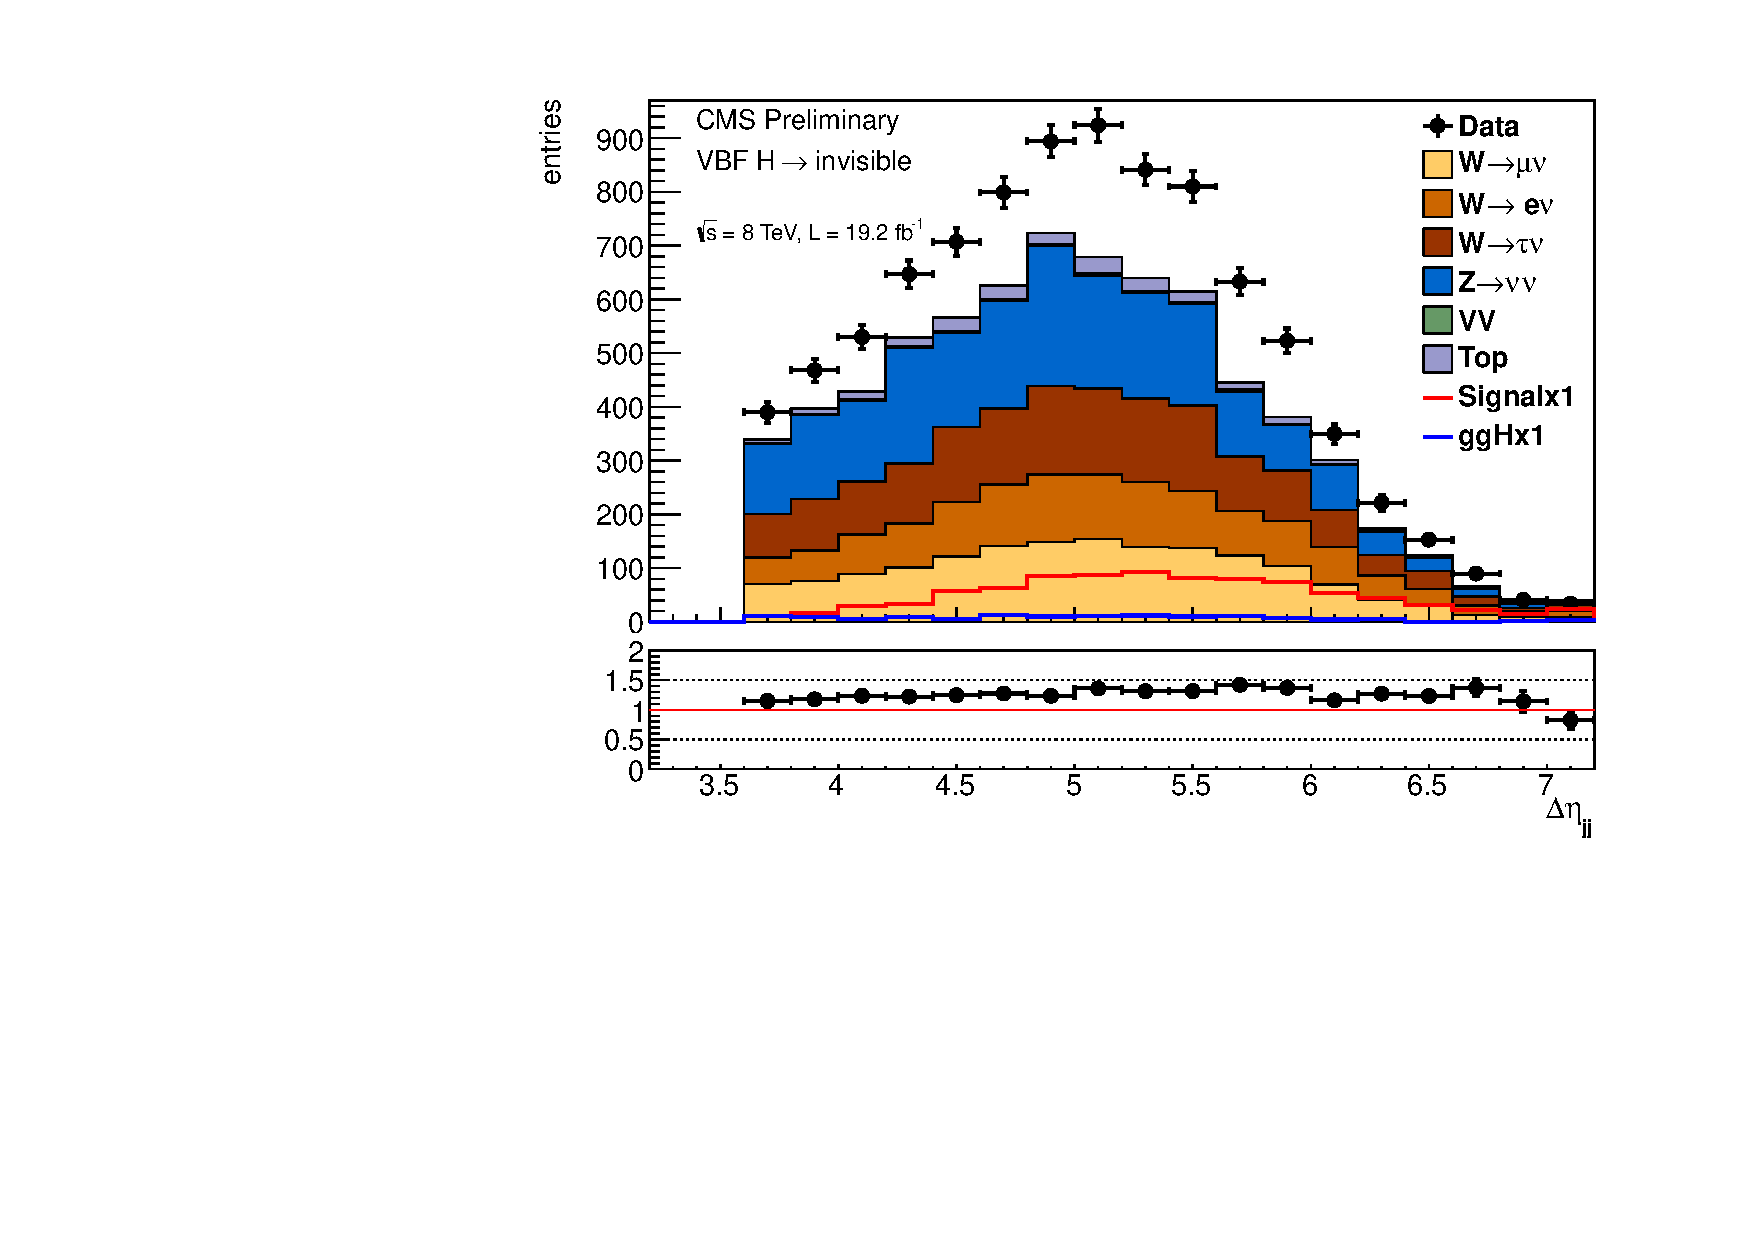
\includegraphics[width=.55\largefigwidth]{plots/parked/AN-14-243-figs/output_presel/nunu_dijet_deta.pdf}}
  \subfloat[]{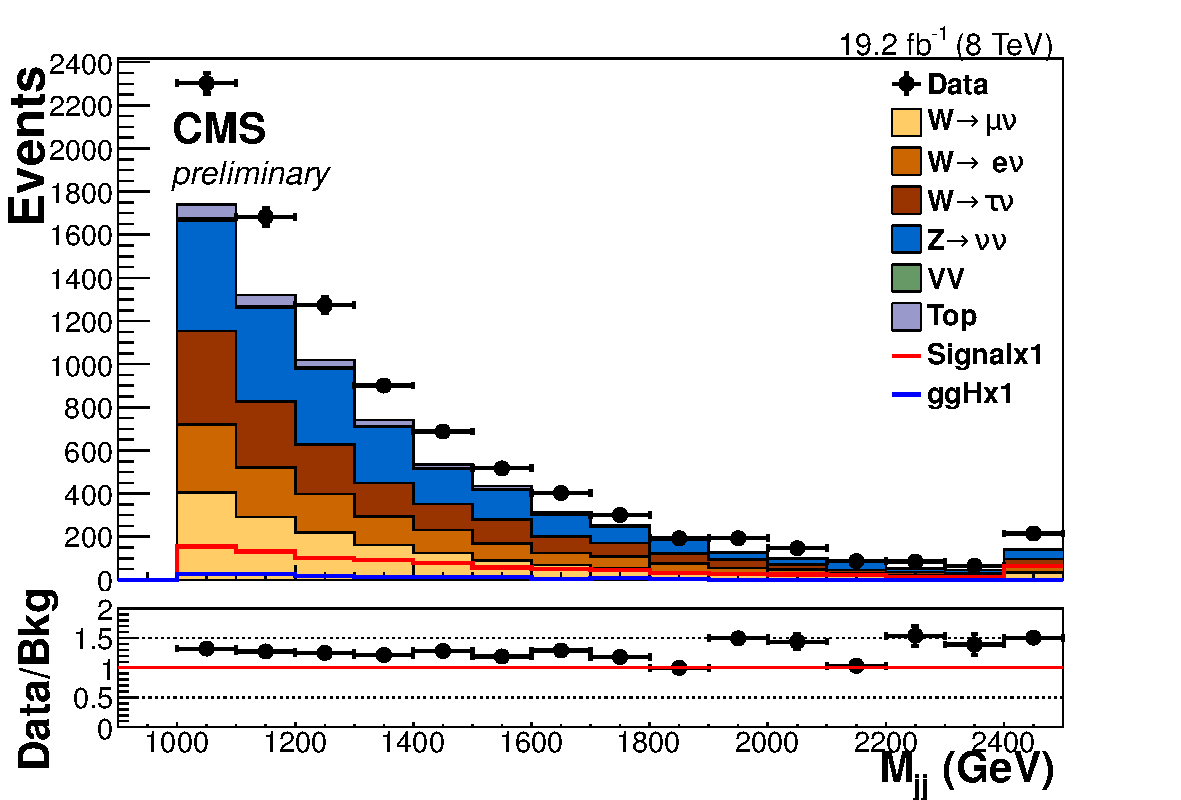
\includegraphics[width=.55\largefigwidth]{plots/parked/AN-14-243-figs/output_presel/nunu_dijet_M.pdf}}
  
  \subfloat[]{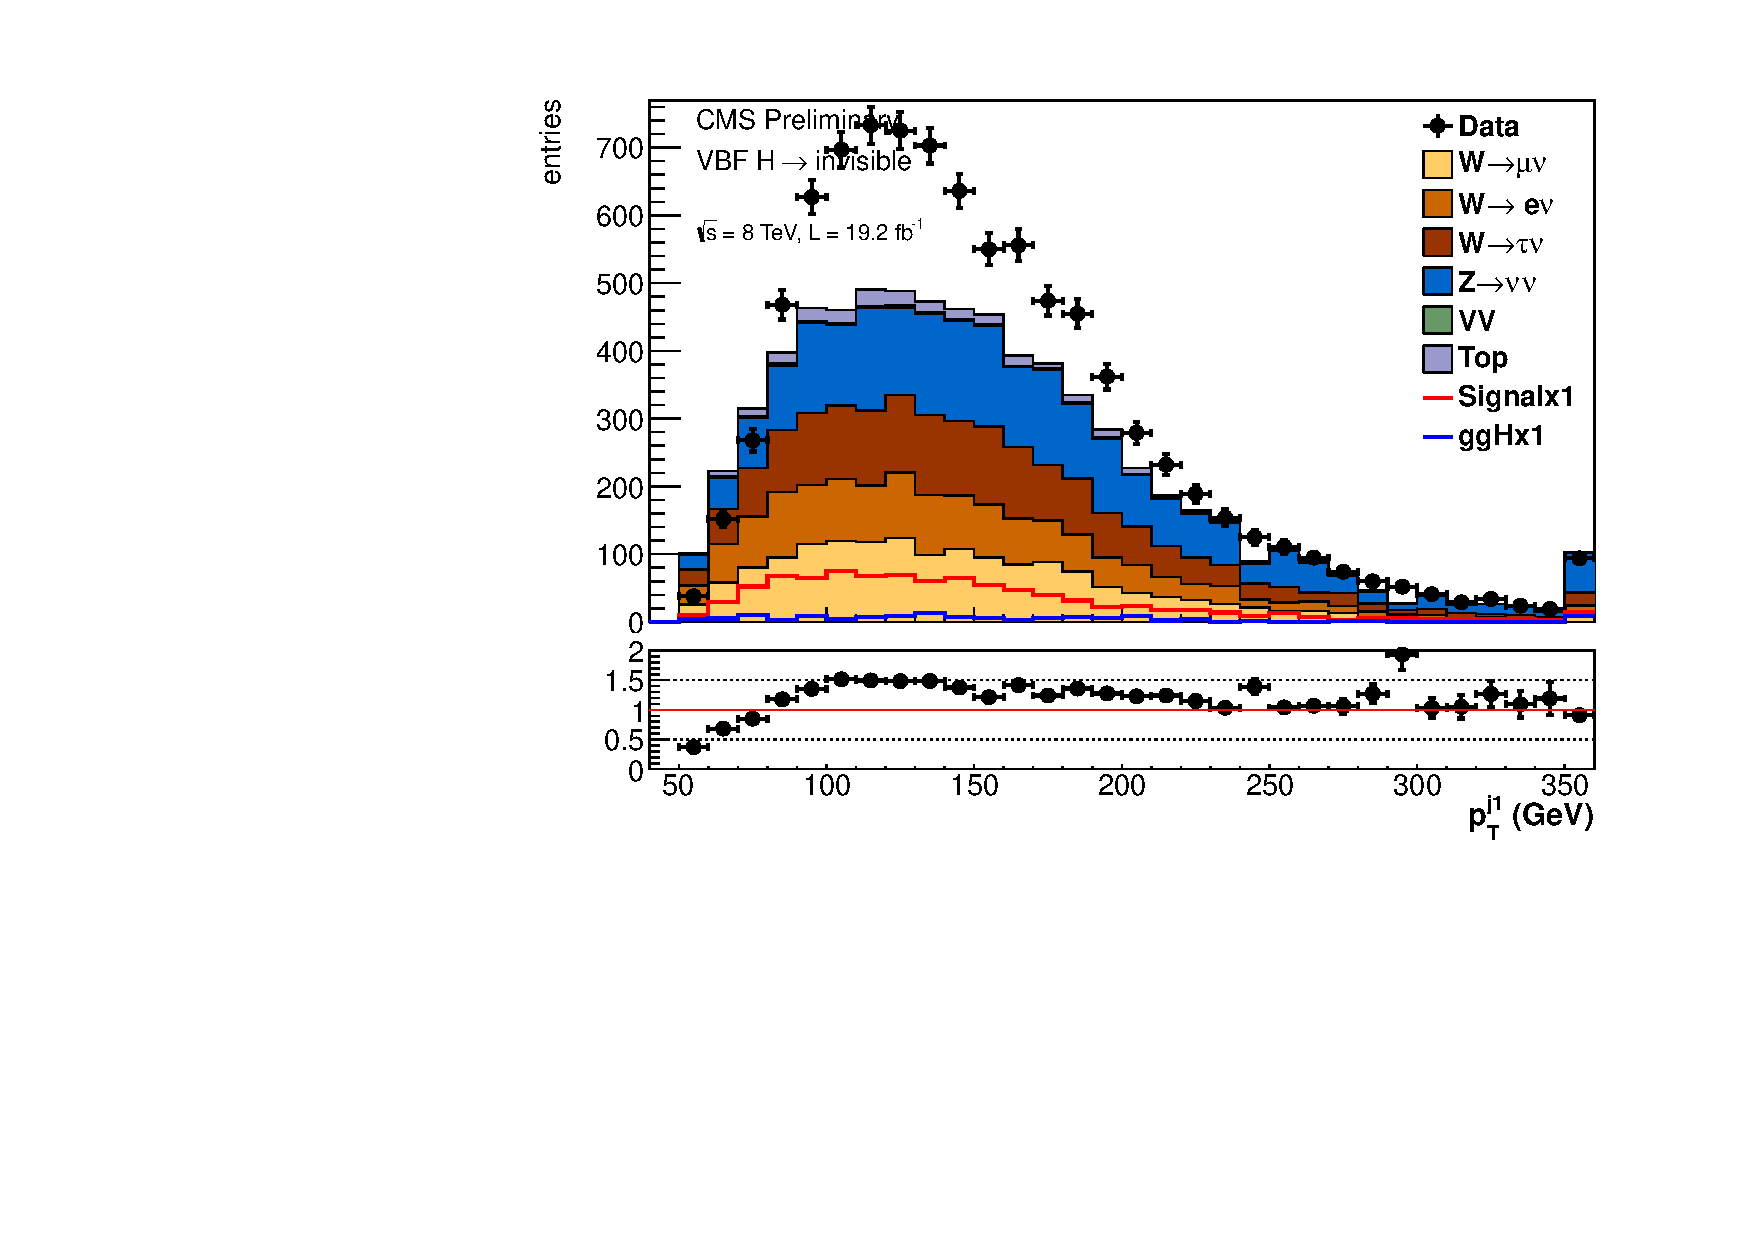
\includegraphics[width=.55\largefigwidth]{plots/parked/AN-14-243-figs/output_presel/nunu_jet1_pt.pdf}}
  \subfloat[]{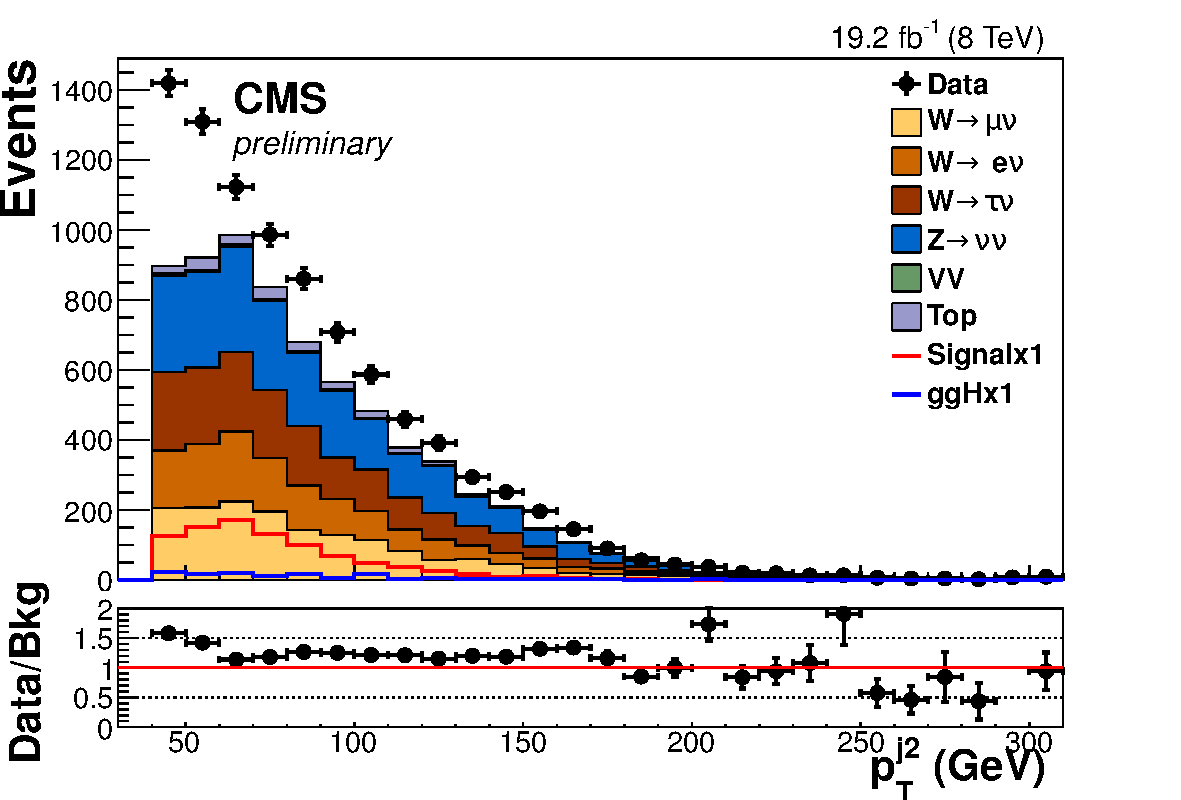
\includegraphics[width=.55\largefigwidth]{plots/parked/AN-14-243-figs/output_presel/nunu_jet2_pt.pdf}}

  \subfloat[]{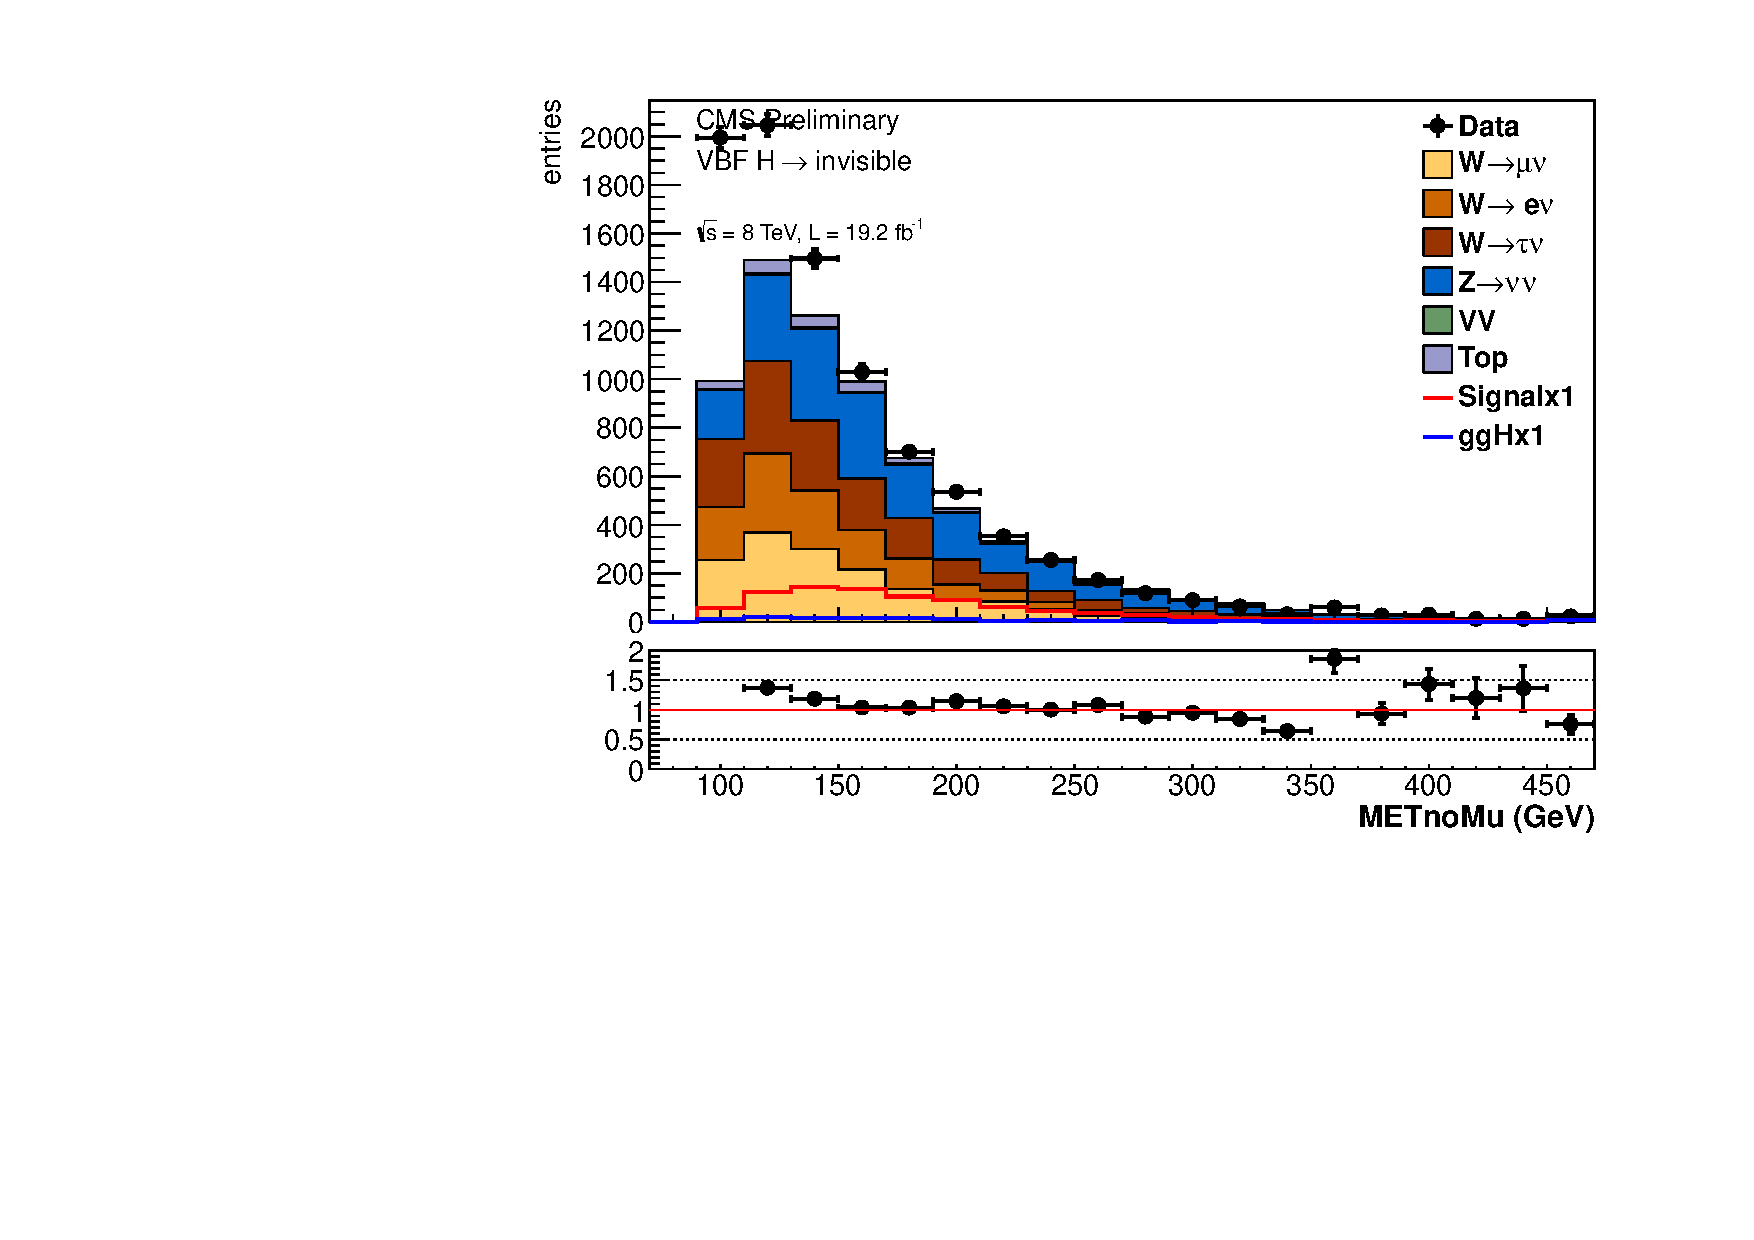
\includegraphics[width=.55\largefigwidth]{plots/parked/AN-14-243-figs/output_presel/nunu_metnomuons.pdf}}
  \subfloat[]{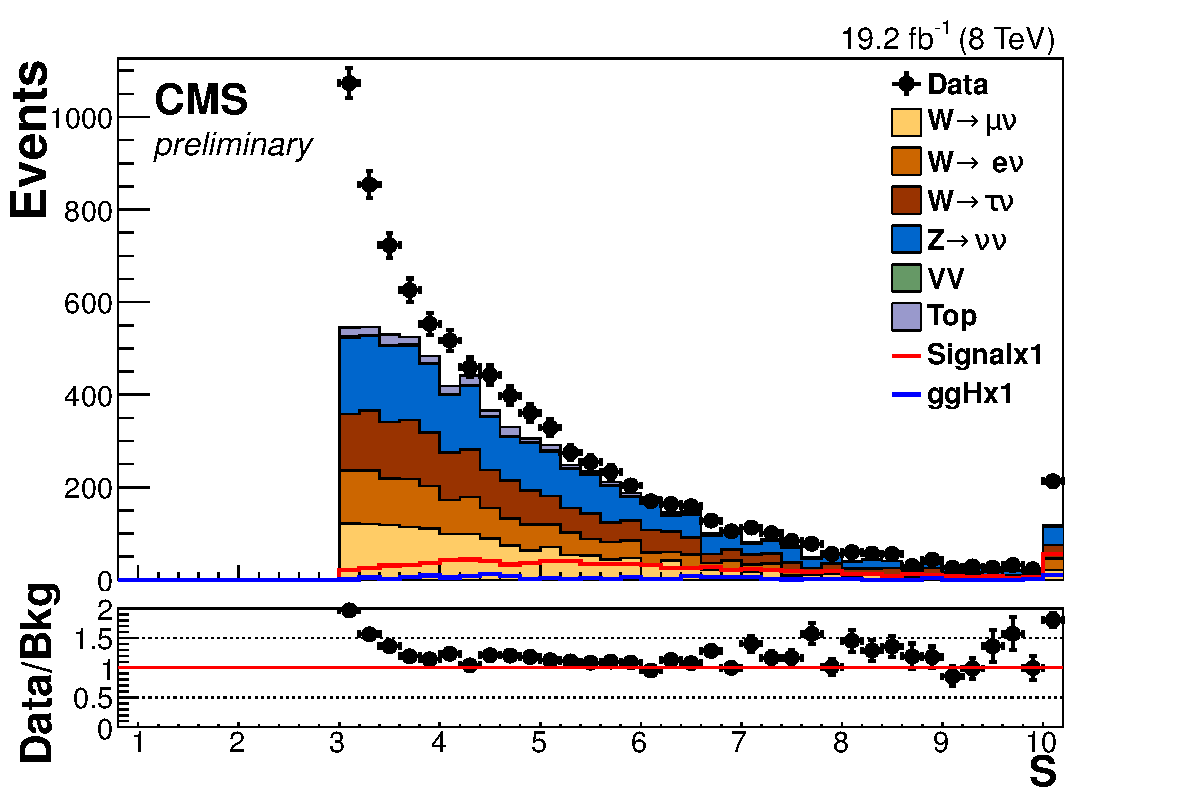
\includegraphics[width=.55\largefigwidth]{plots/parked/AN-14-243-figs/output_presel/nunu_metnomu_significance.pdf}}
  
  \subfloat[]{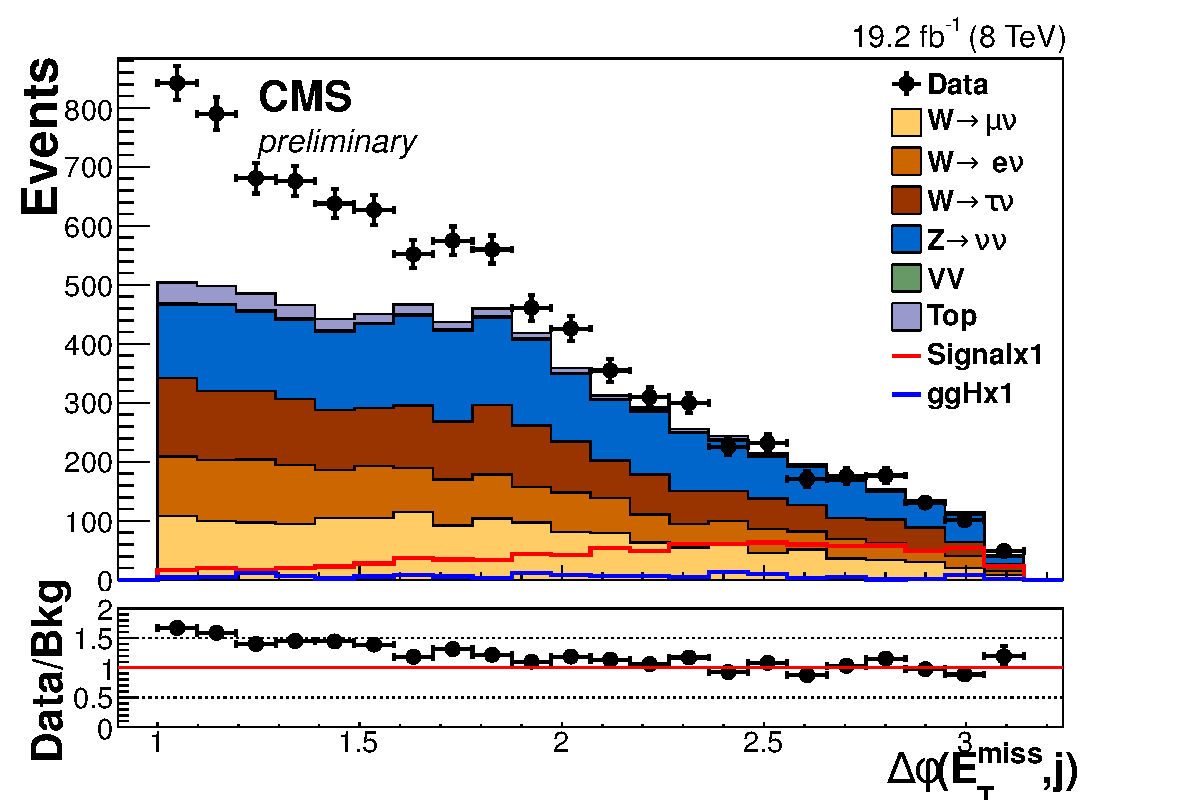
\includegraphics[width=.55\largefigwidth]{plots/parked/AN-14-243-figs/output_presel/nunu_alljetsmetnomu_mindphi.pdf}}

  \caption{From top to bottom left to right distributions of \detajj, \Mjj, leading jet \pt, sub-leading jet \pt, \METnoMU, \METsig and \jetmetdphi for events passing the full preselection. No \ac{QCD} multijet contribution is shown, which accounts for the difference between the data observation and background prediction.}
  \label{fig:parkedpostpresel}
\end{figure}




\subsection{Signal region selection}
\label{sec:parkedsigsel}
As can be seen from \FigureRef{fig:parkedpostpresel}, there is still a significant difference between the data and the \ac{MC} background prediction. It is also evident that the main areas where disagreement occurs are where contributions from \ac{QCD} multijet backgrounds (which are not modelled in the figure) would be expected to contribute, i.e. at low \METsig and low \jetmetdphi, i.e. with jets close to the \METnoMU. Outside these \ac{QCD}-like regions good agreement between data and \ac{MC} is seen. The approach taken was to place tight requirements on these two variables to reduce the \ac{QCD} multijet background to sub-leading levels. The large uncertainties on any estimates of the number of events from \ac{QCD} multijet processes therefore also become negligible. A requirement that events have $\jetmetdphi>2$ and $\METsig>4$, was therefore imposed. The resulting relatively \ac{QCD}-free ``optimisation'' region was blinded (i.e. the data were not looked at) to use for studies to determine the final signal region selection.

Two methods of signal region selection were investigated. The first method was a cut based selection. Starting from the optimisation region the cuts on \METsig, \jetmetdphi, \detajj, sub-leading jet \pt and \Mjj were varied one at a time and the expected limit for each combination of cuts was calculated. The method described in \SectionRef{sec:stats} was used, with the background estimation techniques and systematic uncertainties described in Sections~\ref{sec:parkedbkg} and \ref{sec:parkedsyst} respectively, to calculate the expected limit. In the case of the \ac{QCD} multijet background, which has only a very small contribution to the signal region, the background estimation was performed once for the optimisation selection and used for all cut values. The estimations for all other background processes were repeated for each set of cuts. After each variable was varied the selection was updated to use the cut value that gave the best expected limit. After all the variables had been varied the process was repeated until no improvement in the expected limit was seen so as to avoid ignoring other better sets of cuts. The cut values that gave the best expected limit define the signal region and are as follows:
\begin{equation}
  \label{eq:parkedsigsel}
  \begin{split}
    \eta_{j1}\cdot\eta_{j2}<0,\detajj>3.6,\,\mathrm{leading\,jet\,\pt}>50 \GeV,\\
    \mathrm{subleading\,jet\,\pt}>45 \GeV, \Mjj>1200 \GeV,\\
    \METnoMU>90 \GeV, \METsig>4.0,\jetmetdphi>2.3.
  \end{split}
\end{equation}
After this selection was defined a second \ac{MVA} based method of optimising the selection was investigated to see if could improve on the cut based selection. \ac{BDT} and fisher %??citation and why bdt and fisher
discriminants were trained using signal and background events passing the signal region selection. The signal region selection was used as the basis for this training so as to ensure that the number of events from \ac{QCD} multijet backgrounds in the studied region was small. The optimisation procedure defined above was then repeated with the value of the discriminant considered as an additional variable. The correlation coefficients between the variables used as inputs to the \ac{MVA} are shown for signal and V+jets background events in \FigureRef{fig:parkedmvacorr}. These variables were chosen as they showed the most difference between signal and background distributions and correlations out of a wide range of variables investigated. Without the addition of any additional systematic uncertainties from the understanding of the variables which were input to the \ac{MVA} the best improvement in the expected limit over that of the signal region was less than 1\%. It was therefore decided to use the cut based selection as the final event selection.
\begin{figure}
  \subfloat[]{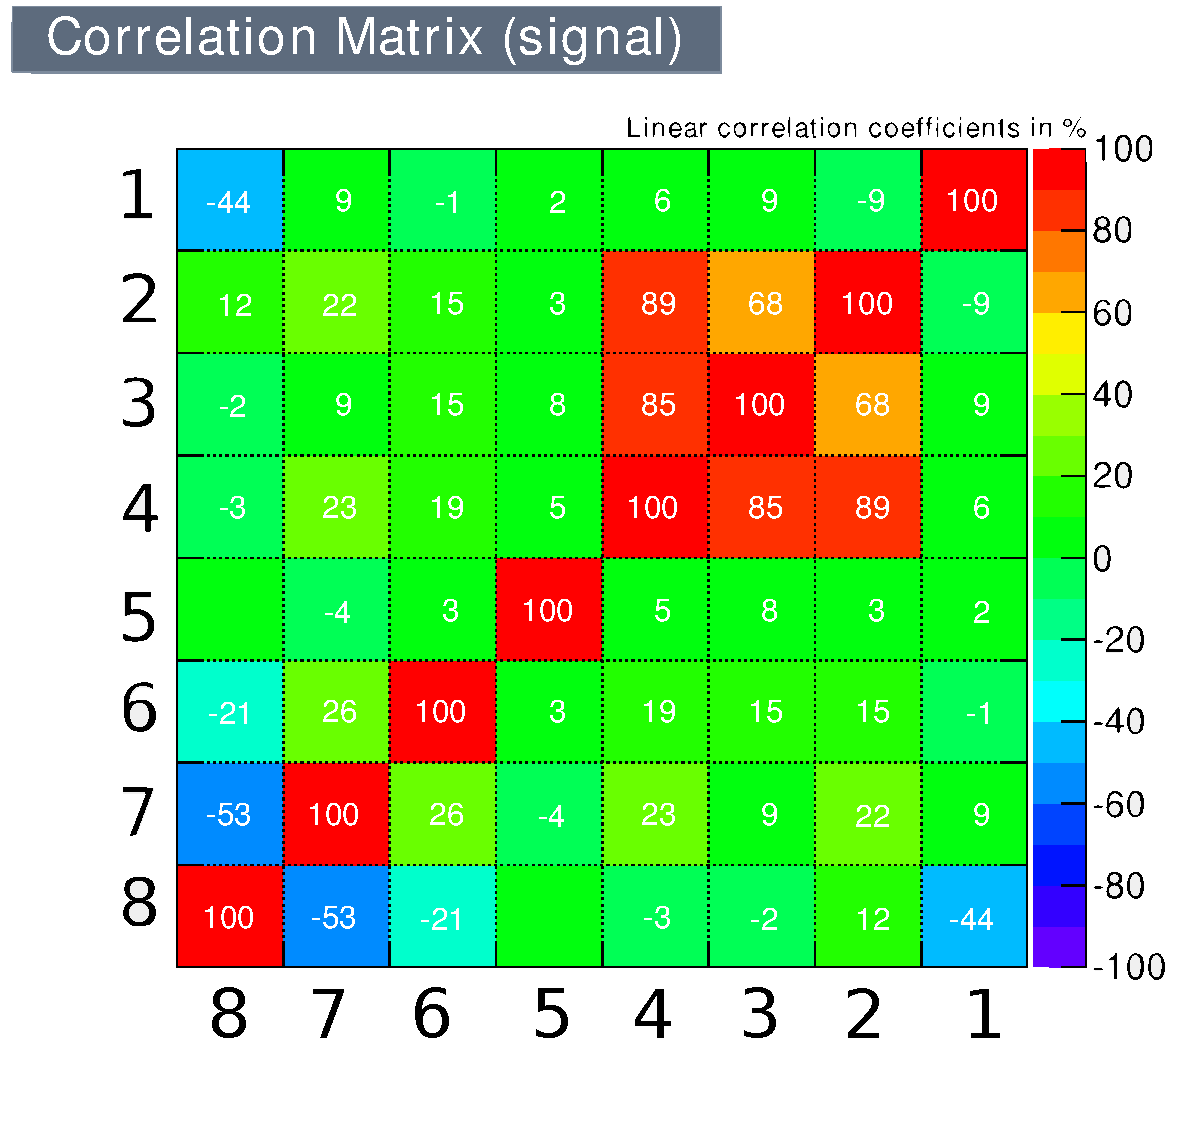
\includegraphics[width=.6\largefigwidth]{plots/parked/AN-14-243-figs/inputcorrsig.pdf}}
  \subfloat[]{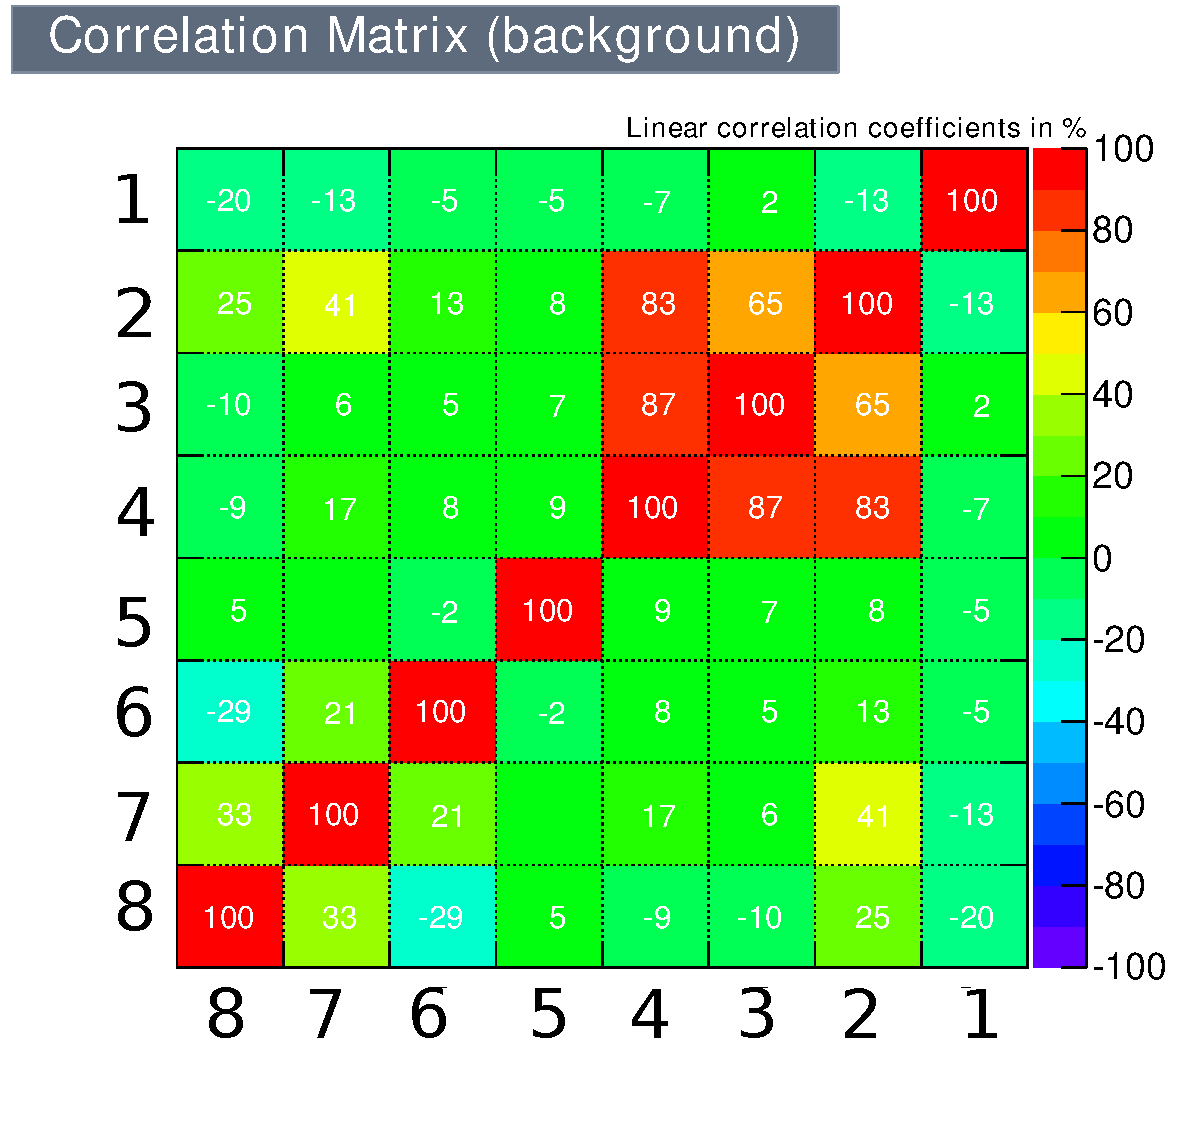
\includegraphics[width=.6\largefigwidth]{plots/parked/AN-14-243-figs/inputcorrbkg.pdf}}
  \caption{Matrices of correlation coefficients for several variables in signal (a) and V+jets background (b) events passing the signal region selection. The variables are 1) the azimuthal angle difference between the \METnoMU and the unclustered energy in the event, 2) the square root of the hadronic energy in the event, 3) \METsig, 4) \METnoMU, 5) \Mjj, 6) the number of jets with $\pt>30$ \GeV between the two tag jets in \eta, 7) the vectorial sum of the tag jets \pt and the \METnoMU, 8) the ratio between the magnitude of the vectorial sum of the tag jet's \pt and the \METnoMU.}
  \label{fig:parkedmvacorr}
\end{figure}

\section{Background estimation}%??                                                                                                                          
\label{sec:parkedbkg}
After selection the V+jets backgrounds, as in the prompt analysis, dominate. Also, as in the prompt data analysis contributions are expected from top quark and diboson related processes. Finally, whilst it is reduced significantly by the selection described above, it is necessary to at least place an upper bound on the expected contribution from \ac{QCD} multijet events.

The methods used to estimate the V+jets backgrounds are based on those used in the prompt data analysis. \EquationRef{eq:wdatabkg} is used in several of these methods in this section, and it is repeated here:
\begin{equation}
  \label{eq:wdatabkgrep}
  N^{S}_{Exp}=\left(N^{C}_{Data}-N^{C}_{Bkg}\right)\cdot\frac{N^{S}_{MC}}{N^{C}_{MC}}.
\end{equation}
The terms on the right hand side of this equation which multiply the estimation from \ac{MC} of the number of events due to a particular background process are often collectively referred to as the data driven scale factor. The changes in event selection for this analysis necessitated several changes from the methods for the prompt analysis. The use of this data driven method to investigate the top quark related background was also investigated. Furthermore, among other improvements, the systematic uncertainty on the \Znunu background was reduced. All of these changes and improvements are described in this section.

\subsection{Top quarks}
Almost all top quarks decay to a \PW boson and a b quark~\cite{pdg}. Top quarks are either created in pairs, or via ``single top'' production where only one top quark is created in association with  other quarks or a \PW boson. Top pair production results in two \PW bosons and two b quarks. Single top production results in some combination of \PW bosons and quarks. Where at least one of the \PW bosons decays leptonically and the lepton is misreconstructed, either of these processes can result in the appearance of \MET and jets that can coincidentally have \ac{VBF}-like topology. Whilst the contribution from these processes is expected to be small in the signal region, making up around 1\% of events there, the presence of \PW bosons and jets makes these processes very likely to contribute to the control regions used to estimate the \PW+jets background contribution. In the $\PW\rightarrow\tau\nu$ control region approximately 15\% of events are estimated to come from top quark processes. Data driven methods for estimating the top quark background and its uncertainties were therefore investigated.

Initially a dilepton control region was investigated. This had the same cuts on the jet and \MET related variables as the signal region, but the lepton veto was replaced with a requirement that there is exactly one tight electron and one tight muon. This final state would be expected in the case of top quark pair production or single top production with a \PW boson, where both the resulting \PW bosons decay leptonically to different leptons. This region had only single figure numbers of events expected, so the cut on \jetmetdphi was loosened to 0. It can be seen from \FigureRef{fig:parkedtopjetmetdphi} that the ratio between data and MC in this region does not depend significantly on \jetmetdphi. The data driven scale factor obtained from this dilepton region was, within the statistics available, consistent with 1 and a good agreement between data and \ac{MC} was seen in all variables studied.

\begin{figure}
  \subfloat[]{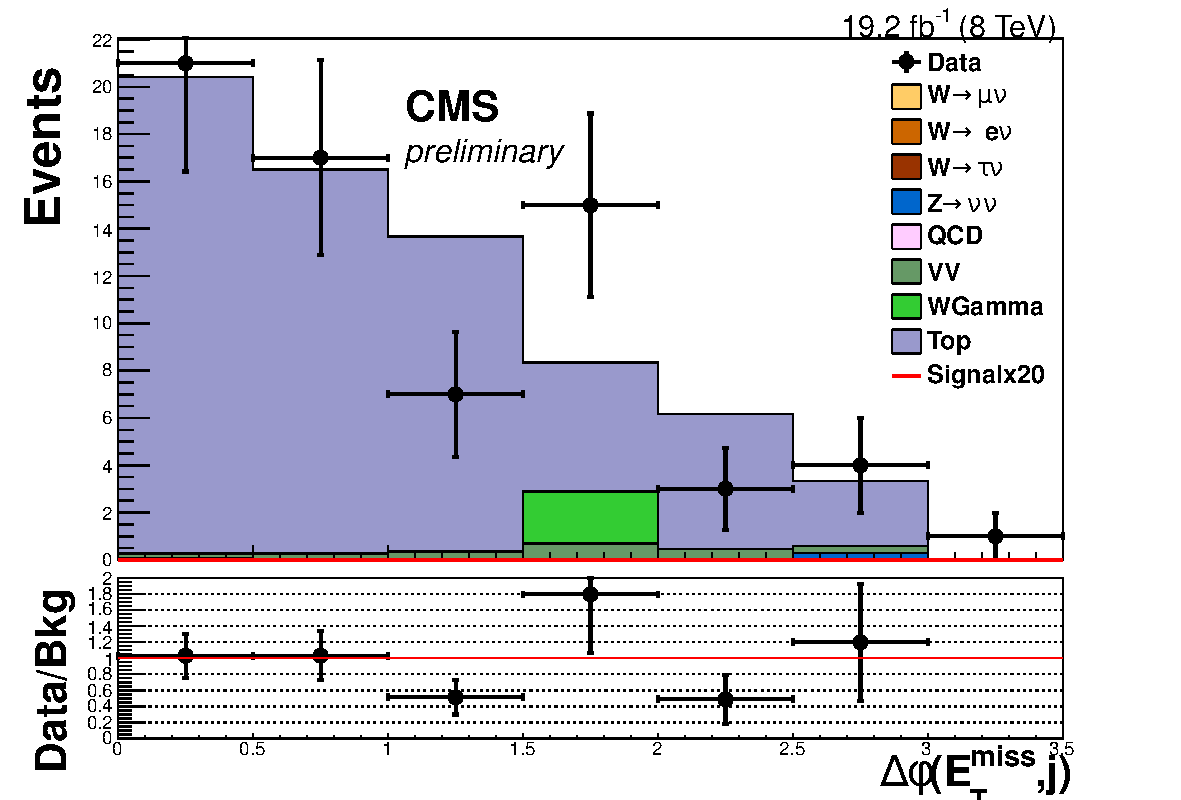
\includegraphics[width=.6\largefigwidth]{plots/parked/topjetmetdphicut0.pdf}}
  \subfloat[]{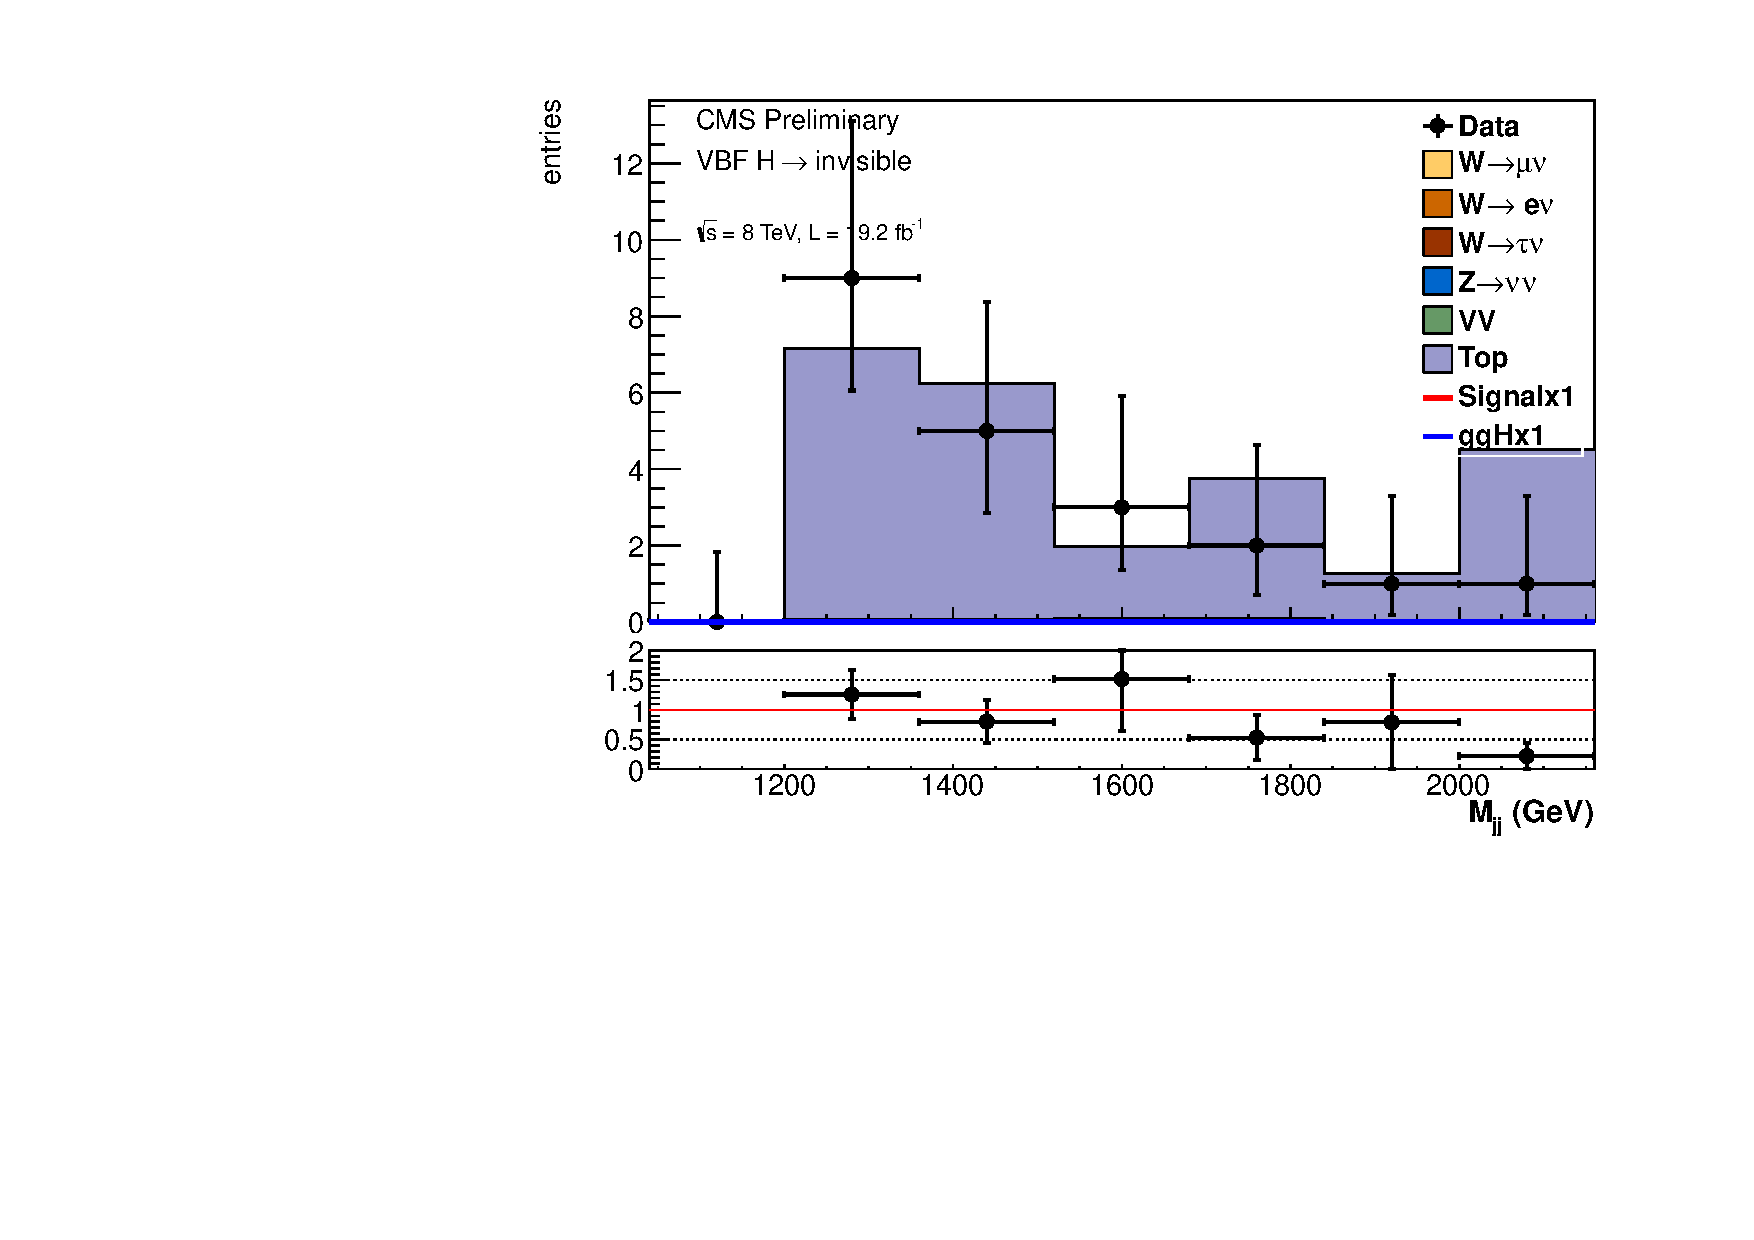
\includegraphics[width=.6\largefigwidth]{plots/parked/AN-14-243-figs/output_sigreg/top_dijet_M.pdf}}
  \caption{The distribution of \jetmetdphi (a) and \Mjj (b) in the top control region with one tight electron and one tight muon.}
  \label{fig:parkedtopjetmetdphi}
\end{figure}

A modification of this control region where events with either two tight electrons or two tight muons, and no other leptons was also studied. This final state would also be expected where two \PW bosons from top quark production decayed leptonically, except this time to the same flavour of lepton. In order to avoid \PZ boson contributions the lepton's invariant mass was required to be incompatible with that of a \PZ boson, i.e. outside of the range from 60 to 120 \GeV. This control region also yielded good data-\ac{MC} agreement and a scale factor compatible with 1. An issue with both of these control regions is that the top quark pair production to single top production ratio is very different to both the signal region and the $\PW\rightarrow\tau\nu$ control region. \ac{MC} estimations indicate that these top control regions have a negligible single top contribution, while the top background in the signal region has almost no top quark pair contribution. The $\PW\rightarrow\tau\nu$ region is expected to be a mixture, its top quark background being 30\% from single top events and 70\% for top quark pairs, again estimated from \ac{MC}. A single top control region was therefore also investigated.

The single top region differed from the signal region in that the \jetmetdphi cut was removed, exactly one tight electron or muon was required, further leptons were vetoed and one of the tag jets was required to be compatible with being a b-jet. The restriction to a single lepton significantly reduces the top quark pair production contribution where both resulting \PW bosons decay leptonically, and the requirement of one b-jet reduces the \PW+jets contribution. 

Identification of the b-jet was done using the \ac{CSV} discriminant. b quarks are both heavier and longer lived than many other particles created at the \LHC, meaning that their secondary decay vertex can be distinguished from the \ac{PV}. \ac{CSV} is an \ac{MVA} based discriminant which uses information on secondary vertices and the lifetime of the particle to discriminate between jets from b quarks and those from other lighter quarks. The medium working point used for this control region correctly has an efficiency of approximately 85\% for b-quarks and mis-identifies lighter quark jets as b jets approximately 1\% of the time~\cite{bjets}.

\ac{MC} estimates indicate the single top region has a 17\% single top contribution. This region again showed good data-\ac{MC} agreement and a scale factor compatible with 1 within uncertainties. Because good agreement between data and \ac{MC} and scale factors compatible with 1 are seen in all investigated control regions, it was decided to use the \ac{MC} prediction for the top background in all regions with no additional scale factor. A 20\% systematic uncertainty was applied to this prediction which covered the largest deviation from 1 seen in the scale factors from the various control regions.

\begin{figure}
  \subfloat[]{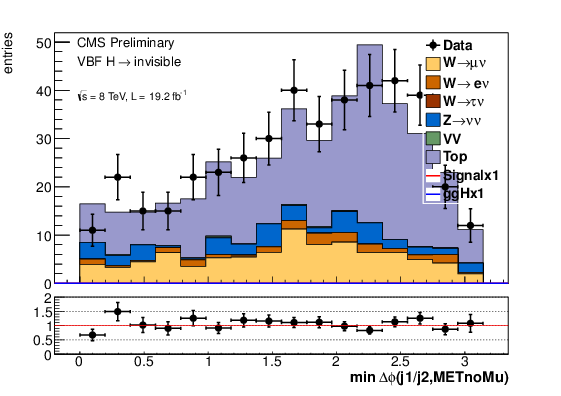
\includegraphics[width=.6\largefigwidth]{plots/parked/AN-14-243-figs/singletop/top_jetmetnomu_mindphi.png}}
  \subfloat[]{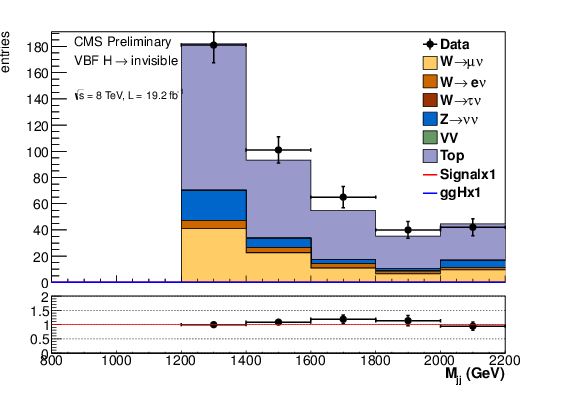
\includegraphics[width=.6\largefigwidth]{plots/parked/AN-14-243-figs/singletop/top_dijet_M.png}}
  \caption{The distribution of \jetmetdphileading (a) and \Mjj (b) in the single top control region.}
  \label{fig:parkedtopjetmetdphi}
\end{figure}

\subsection{W$\rightarrow e\nu$+jets}%??                                                                                                                    
\label{sec:parkedwenu}
The $\PW\rightarrow e\nu$ background in the parked data analysis is estimated using the same method as that used for the prompt data analysis being based on \EquationRef{eq:wdatabkgrep}. The control region used has the same requirements as the signal region, except that the electron veto is replaced with a requirement that there is one tight electron and no other electrons present in the event. The requirement of an electron removes signal events and enriches the region in $\PW\rightarrow e\nu$ events. The distributions of several variables in data and \ac{MC} (which has been scaled by the data driven scale factor extracted from this control region) are shown in \FigureRef{fig:parkedwenu}, where good agreement can be seen. A table of the inputs to and results of \EquationRef{eq:wdatabkgrep} can be seen in \TableRef{tab:parkedwenu}. The table also shows that the expected contribution to this region from other background processes is small, being approximately 5\%. The scale factor obtained for this background is 0.5, which is significantly different from 1, this difference is further investigated in \SectionRef{sec:parkedscalefactors}.

\begin{table}
  \begin{center}
    \caption{The inputs to and results of \EquationRef{eq:wdatabkgrep}, when used to estimate the $W\rightarrow e\nu$ estimate in the signal
      region.}
    \label{tab:parkedwenu}
    \begin{tabular}{lcc}
      \hline
      \hline
      & Signal region & Control region \\
      \hline
      \hline
      $N_{Data}$&N/A&$68\pm 8.2$\stat\\
      $N_{Bkg}$&N/A&$3.5\pm 1.2(MC stat)$\\
      $N_{MC}$&$114.9\pm8.9(MC stat)$&$128.0\pm 8.0(MC stat)$\\
      \hline
      $\frac{N^{data}-N^{bkg}}{N^{W MC}_{C}}$ & \multicolumn{2}{c|}{$0.50\pm0.06$\stat$\pm0.03$(MC stat.)} \\
      \hline
      $N_{\PW\rightarrow e\nu}$&\textcolor{red}{$57.9\pm7.4$\stat$\pm7.7$\syst}&N/A \\
        \hline
        \hline
    \end{tabular}
  \end{center}
\end{table}

\begin{figure}
  \subfloat[]{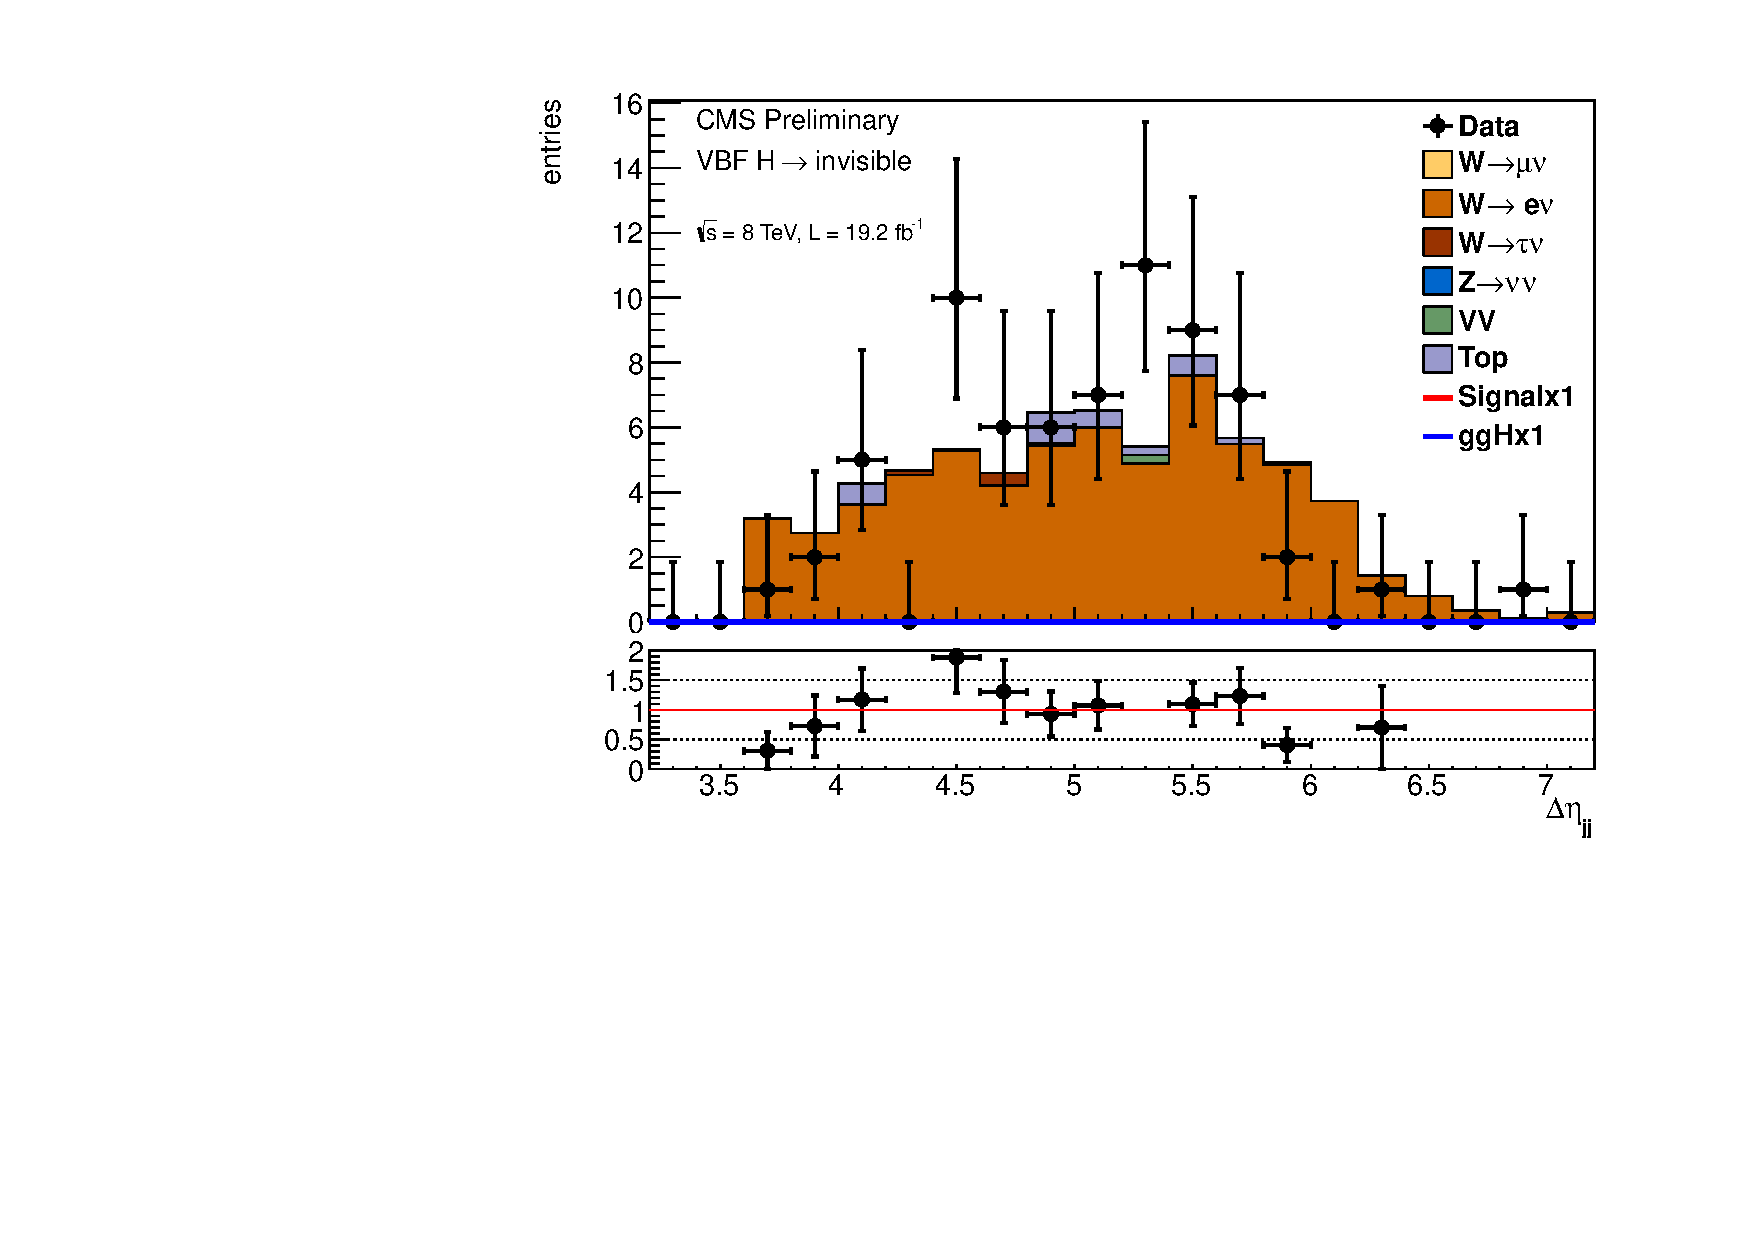
\includegraphics[width=.55\largefigwidth]{plots/parked/AN-14-243-figs/output_sigreg/enu_dijet_deta.pdf}}
  \subfloat[]{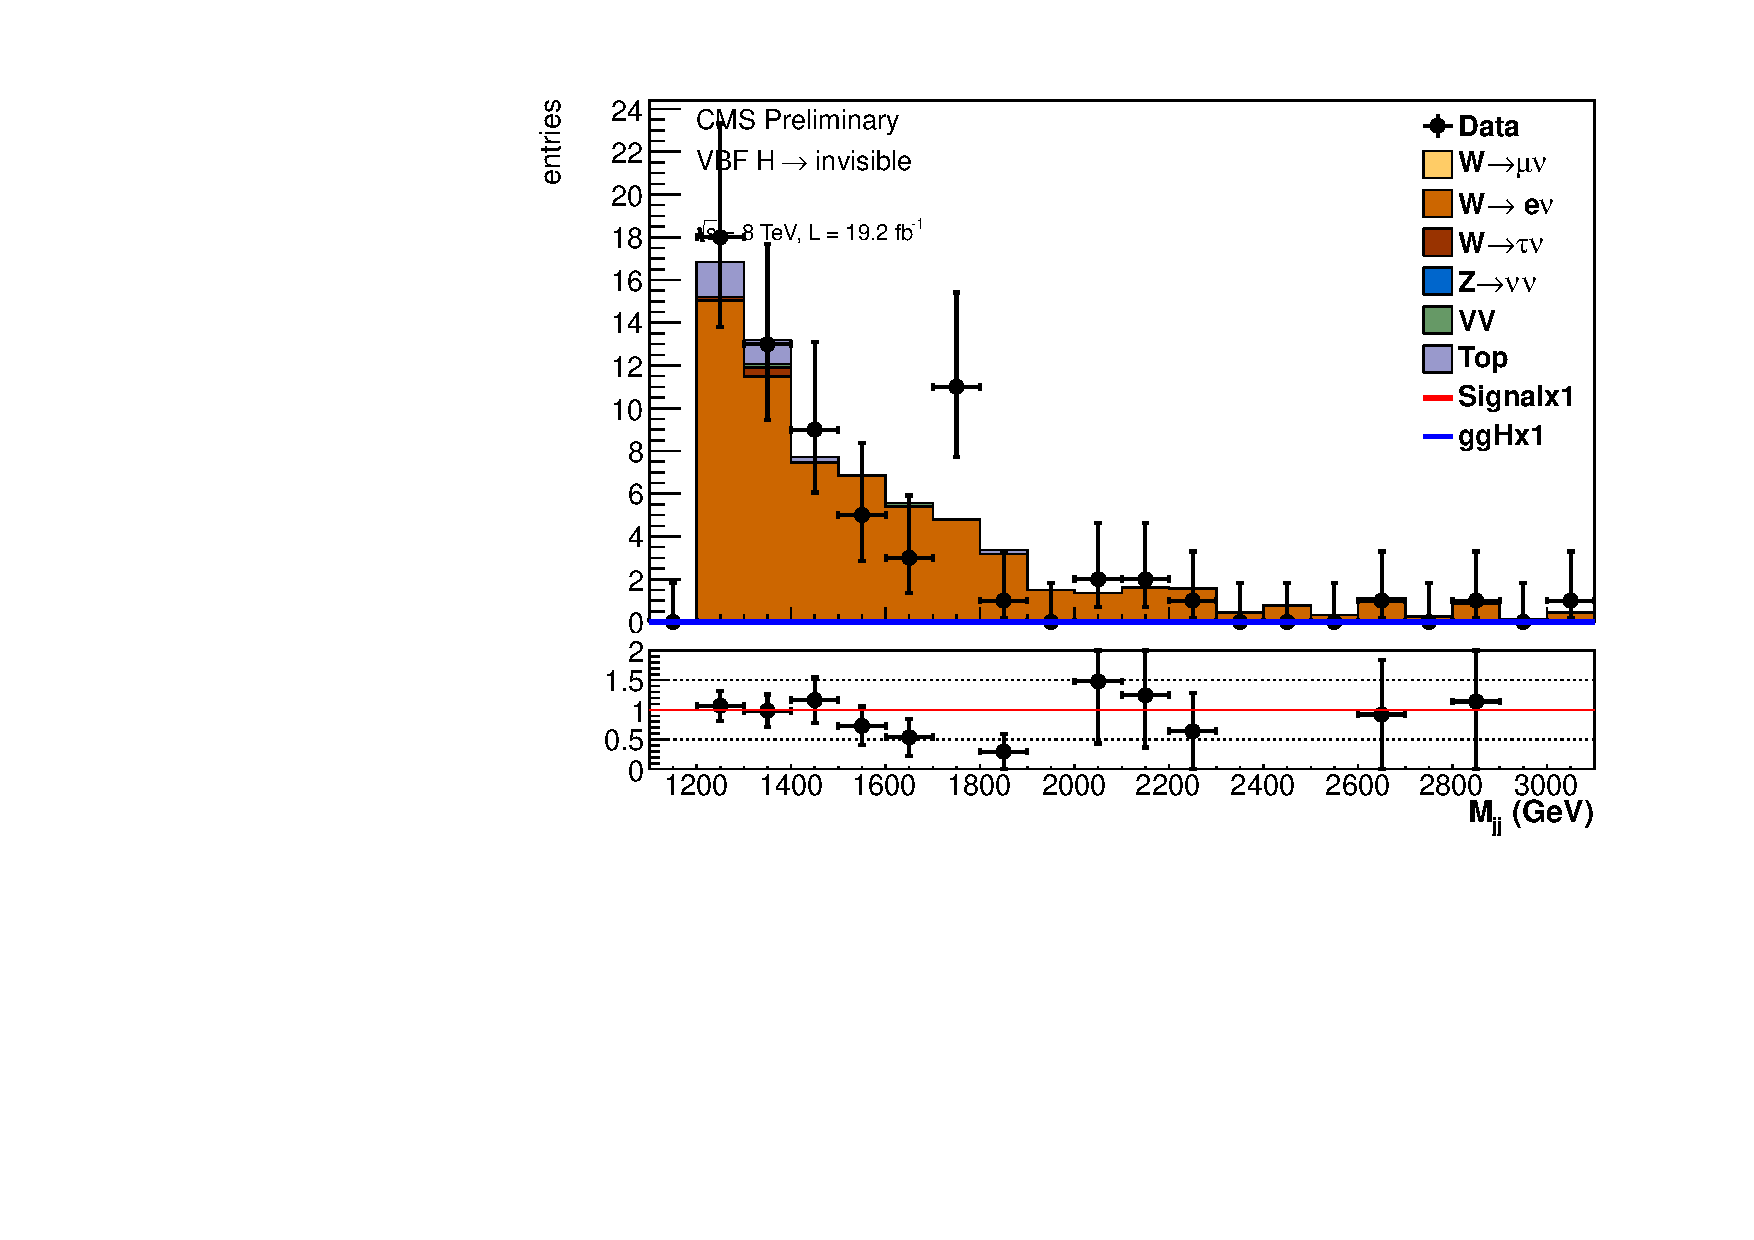
\includegraphics[width=.55\largefigwidth]{plots/parked/AN-14-243-figs/output_sigreg/enu_dijet_M.pdf}}
 
  \subfloat[]{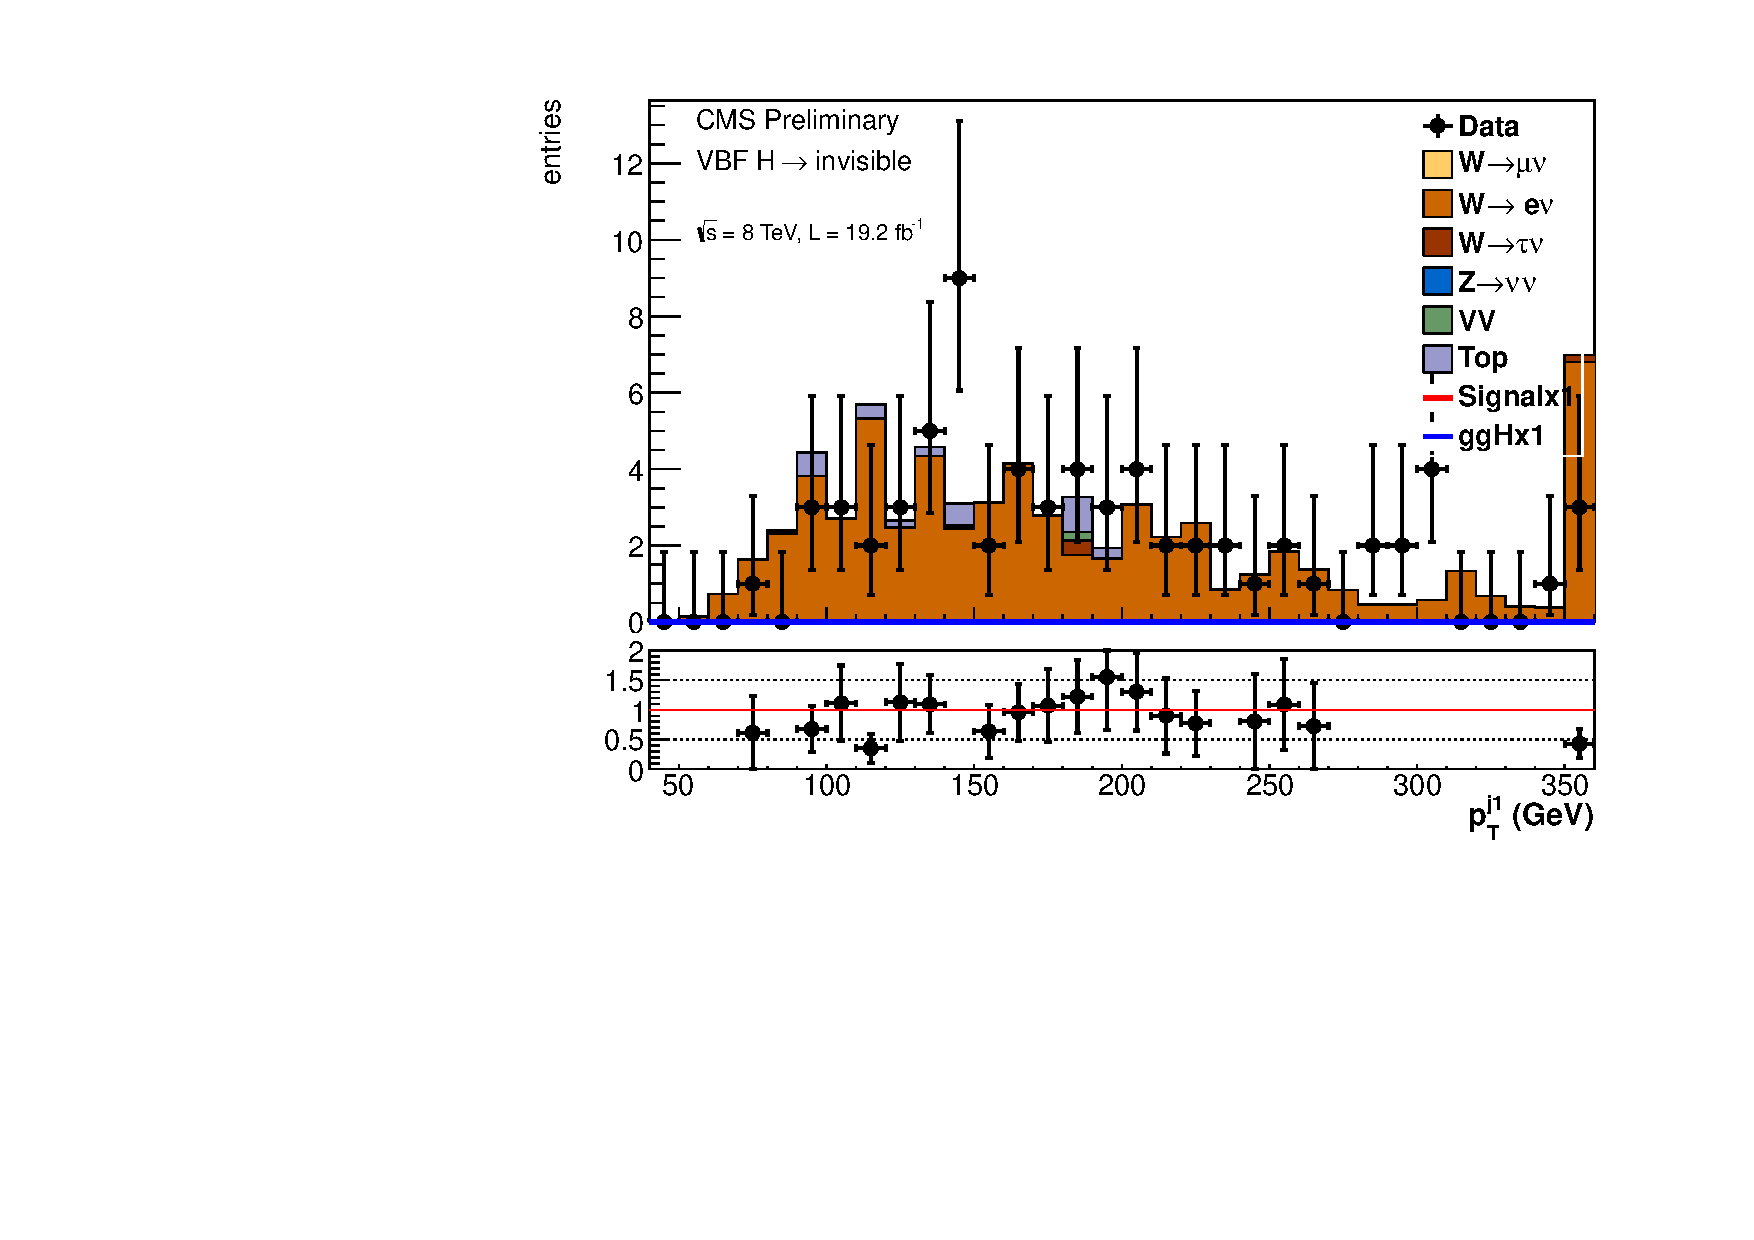
\includegraphics[width=.55\largefigwidth]{plots/parked/AN-14-243-figs/output_sigreg/enu_jet1_pt.pdf}}
  \subfloat[]{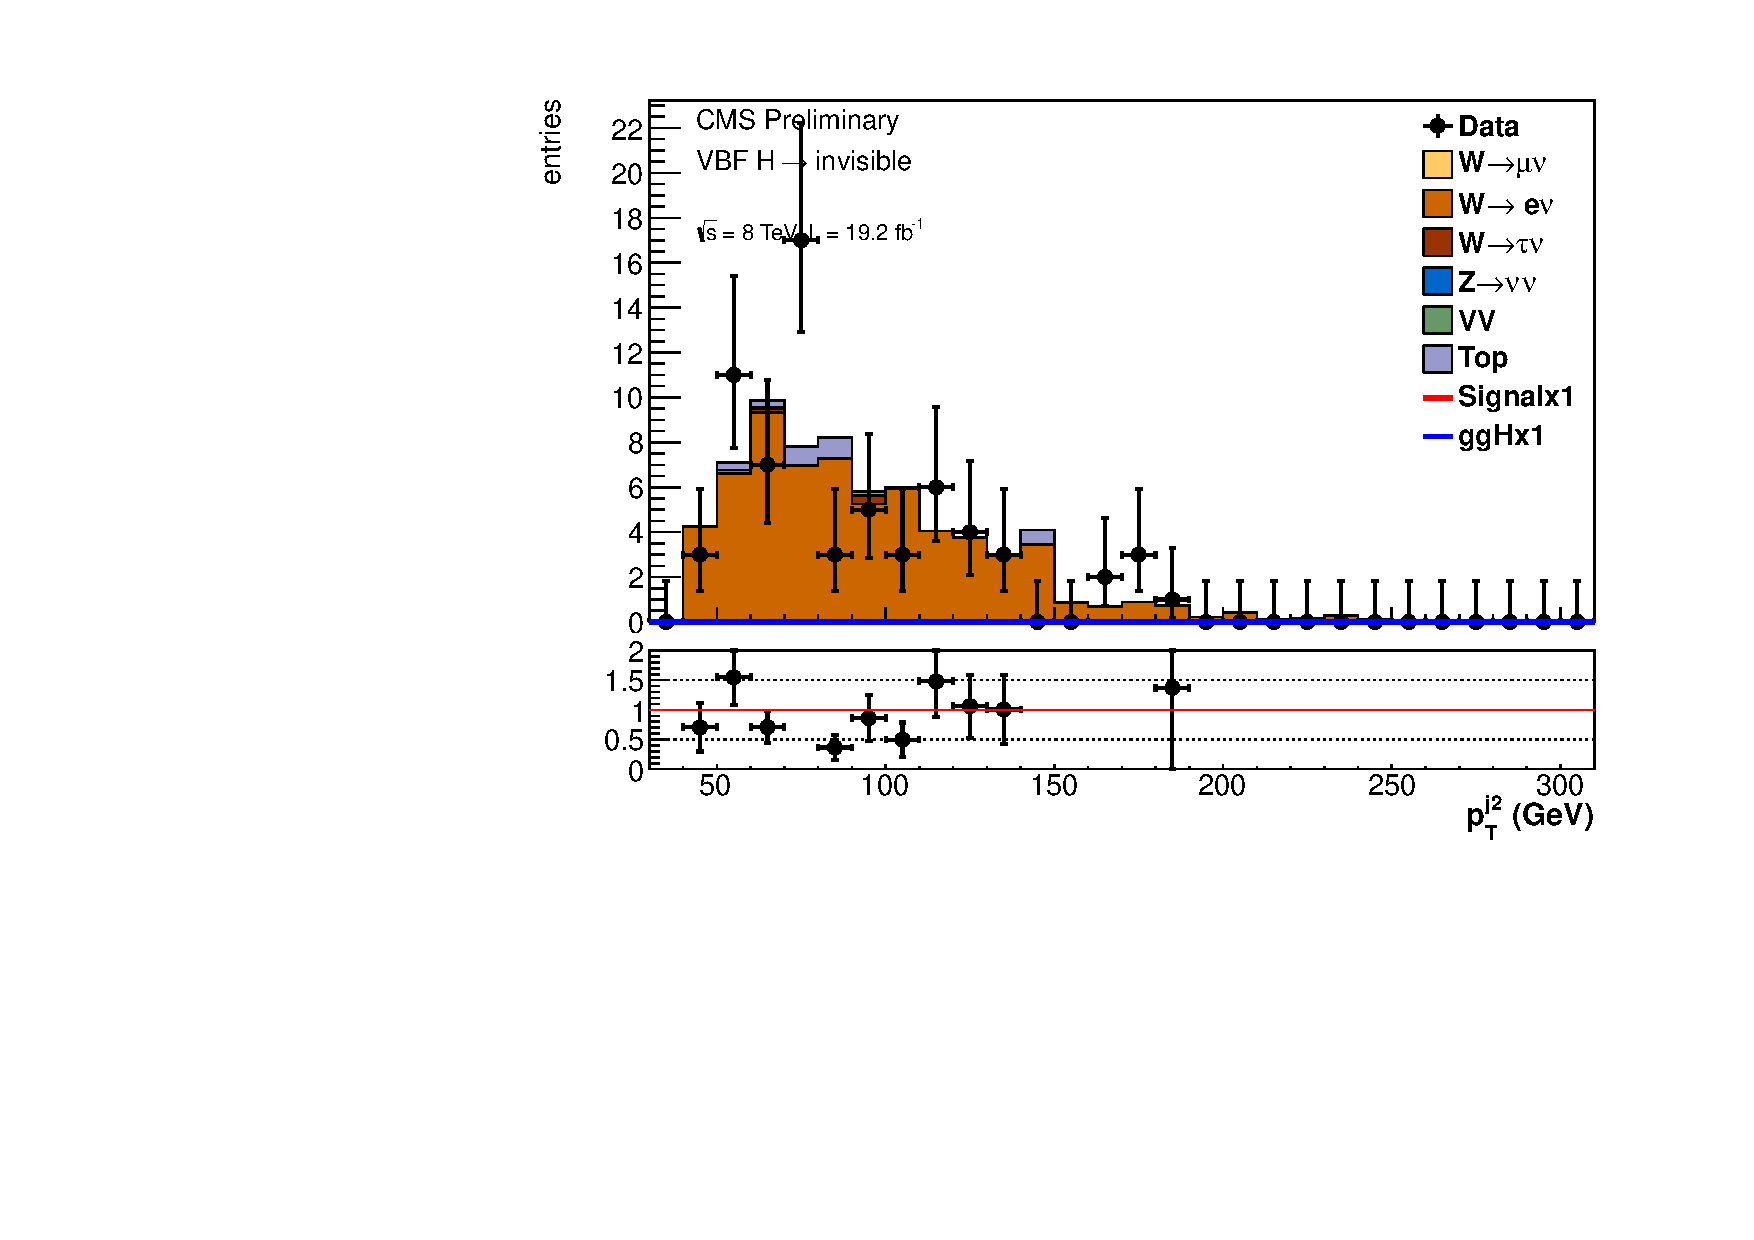
\includegraphics[width=.55\largefigwidth]{plots/parked/AN-14-243-figs/output_sigreg/enu_jet2_pt.pdf}}

  \subfloat[]{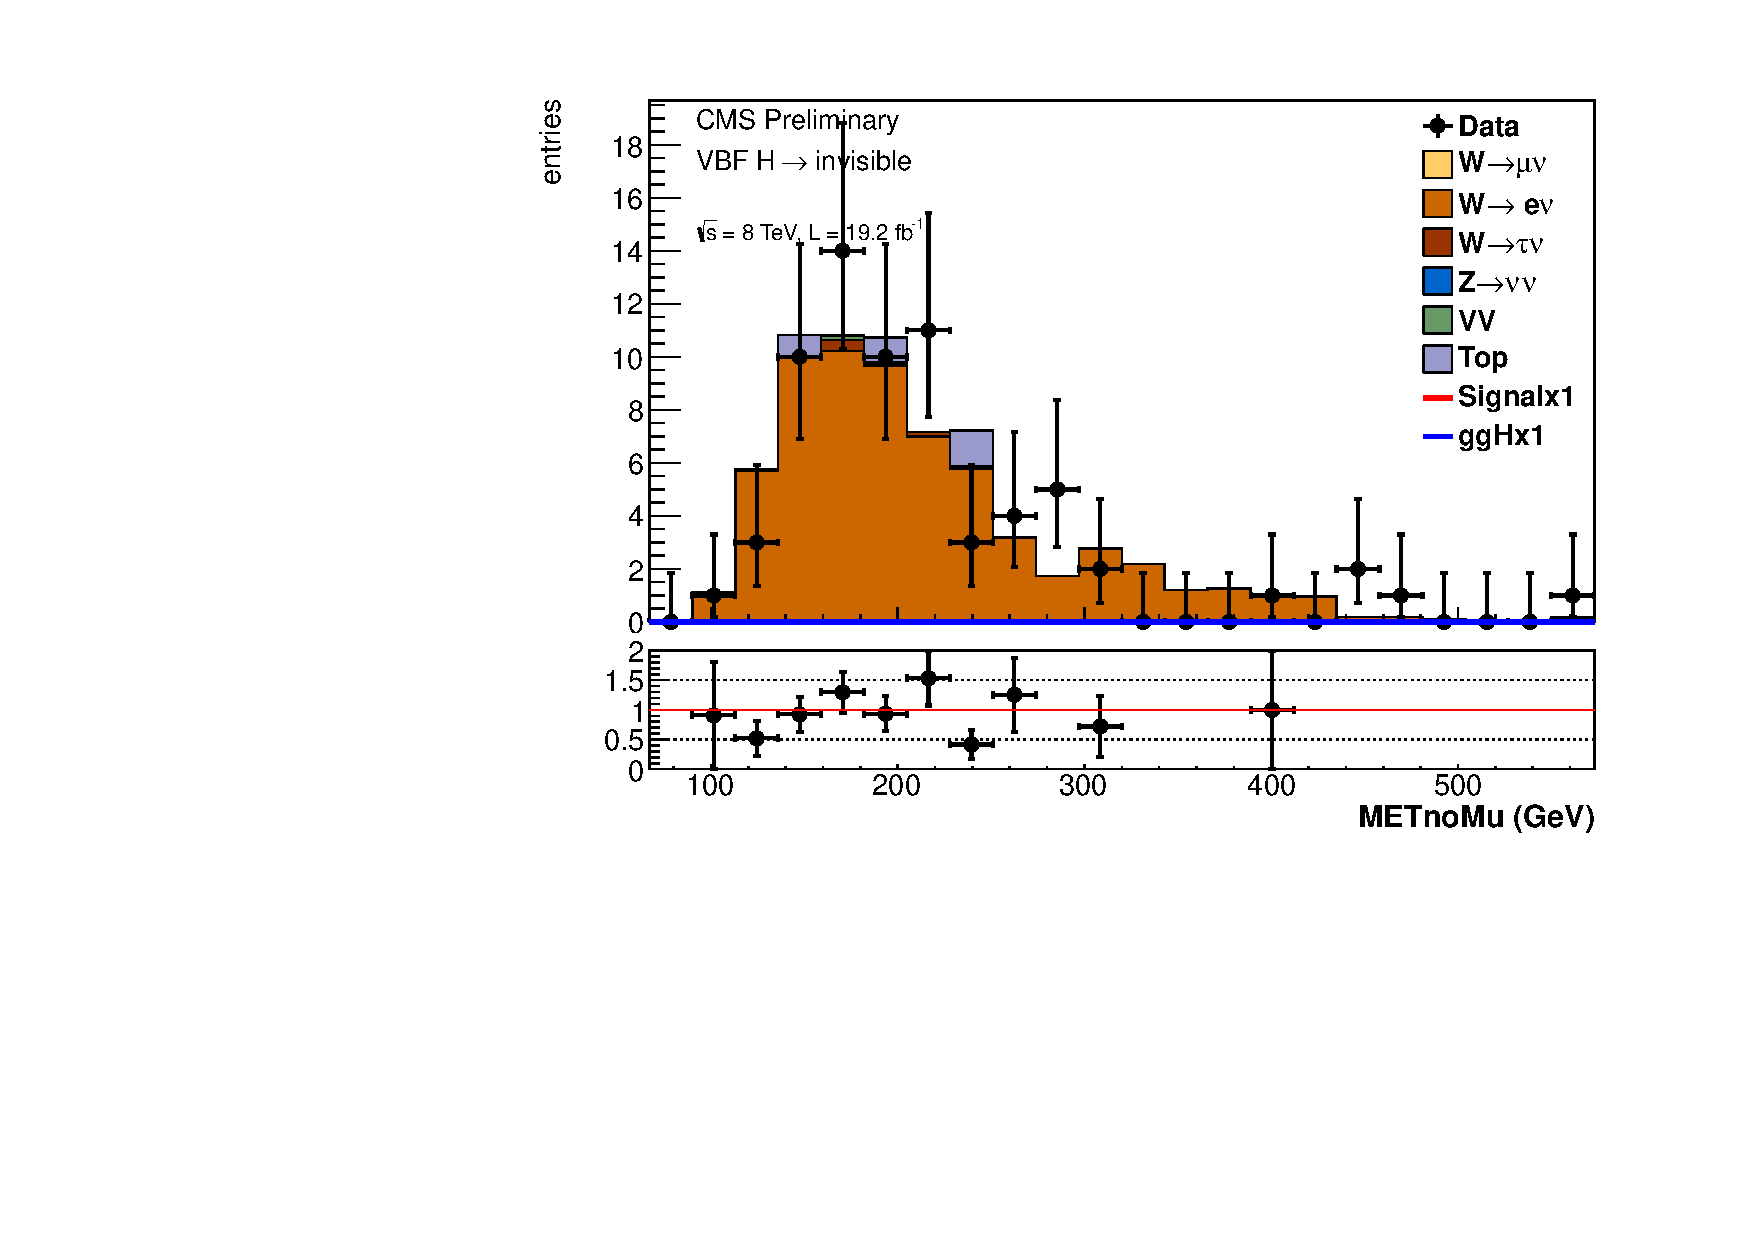
\includegraphics[width=.55\largefigwidth]{plots/parked/AN-14-243-figs/output_sigreg/enu_metnomuons.pdf}}
  \subfloat[]{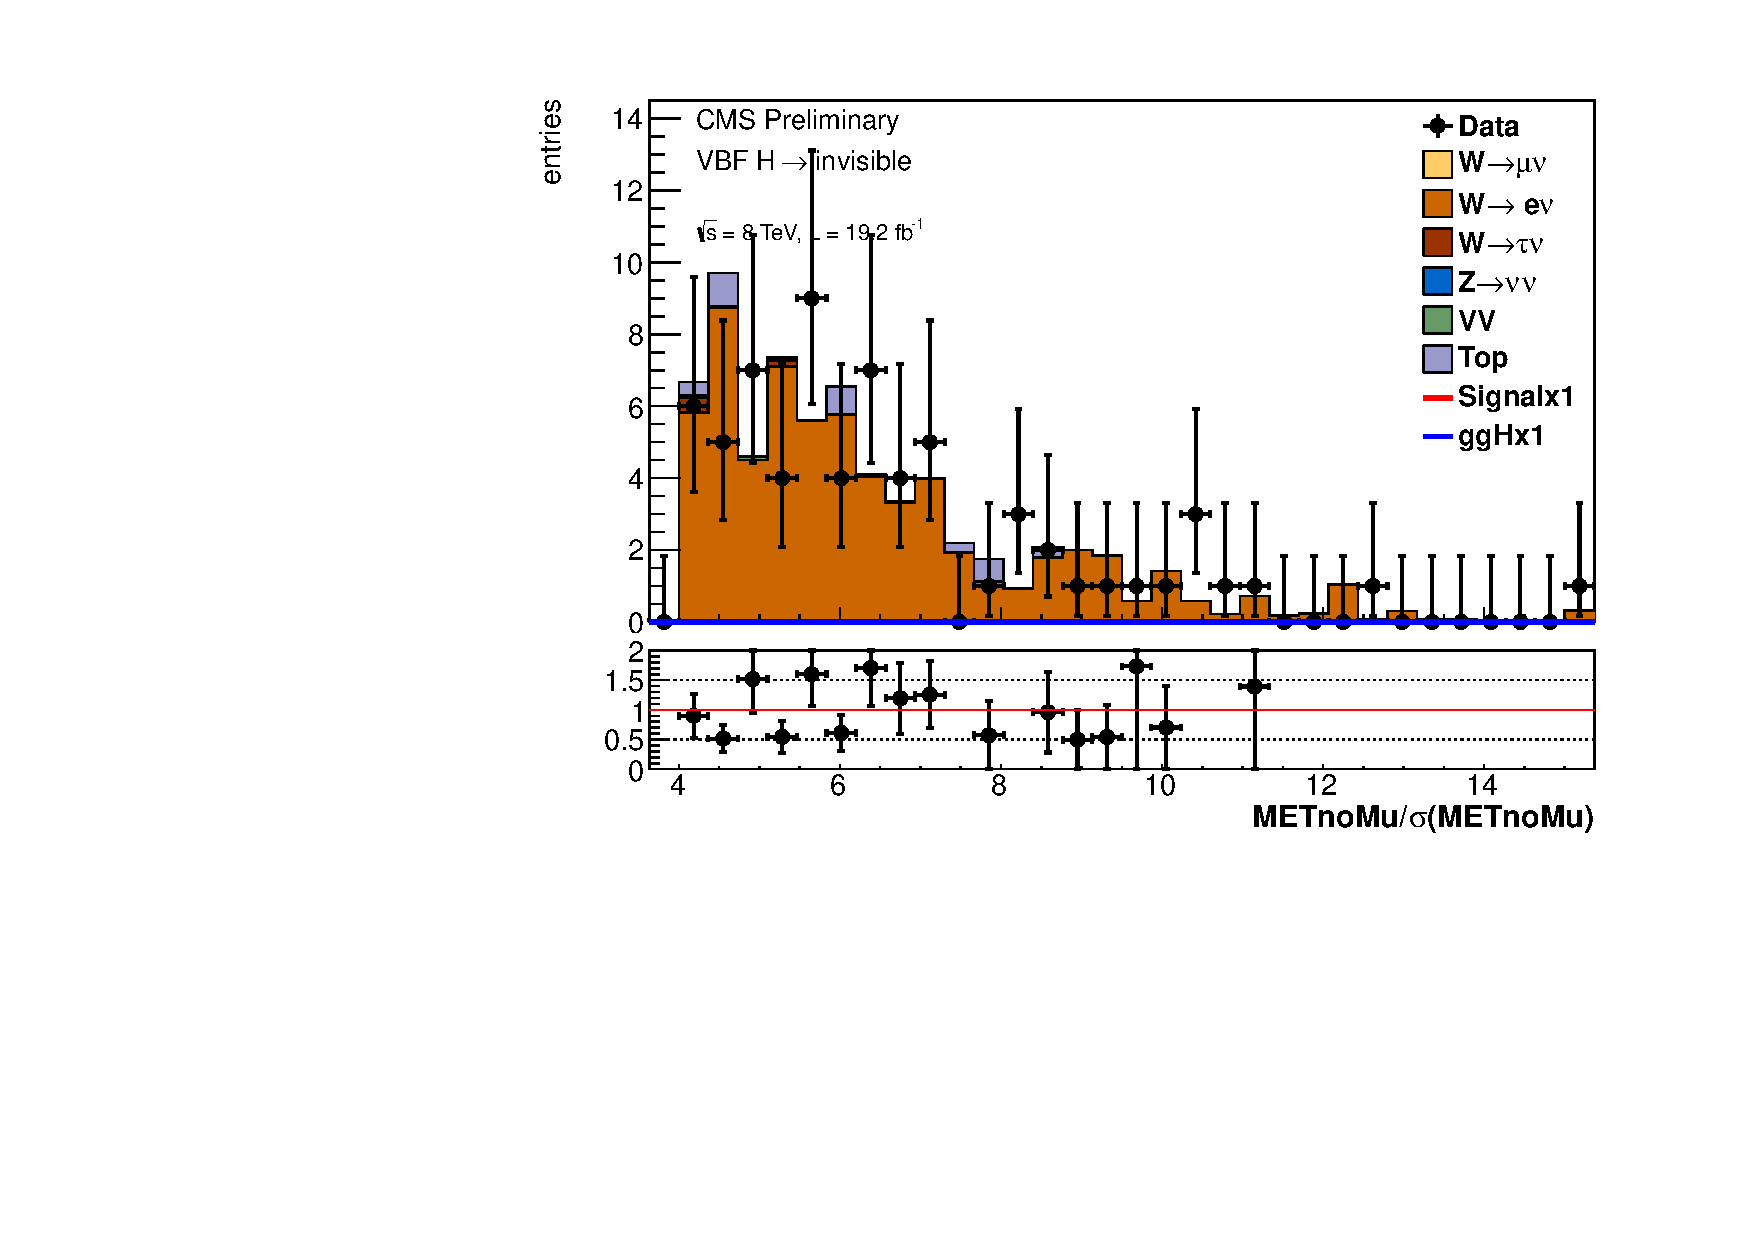
\includegraphics[width=.55\largefigwidth]{plots/parked/AN-14-243-figs/output_sigreg/enu_metnomu_significance.pdf}}
  
  \subfloat[]{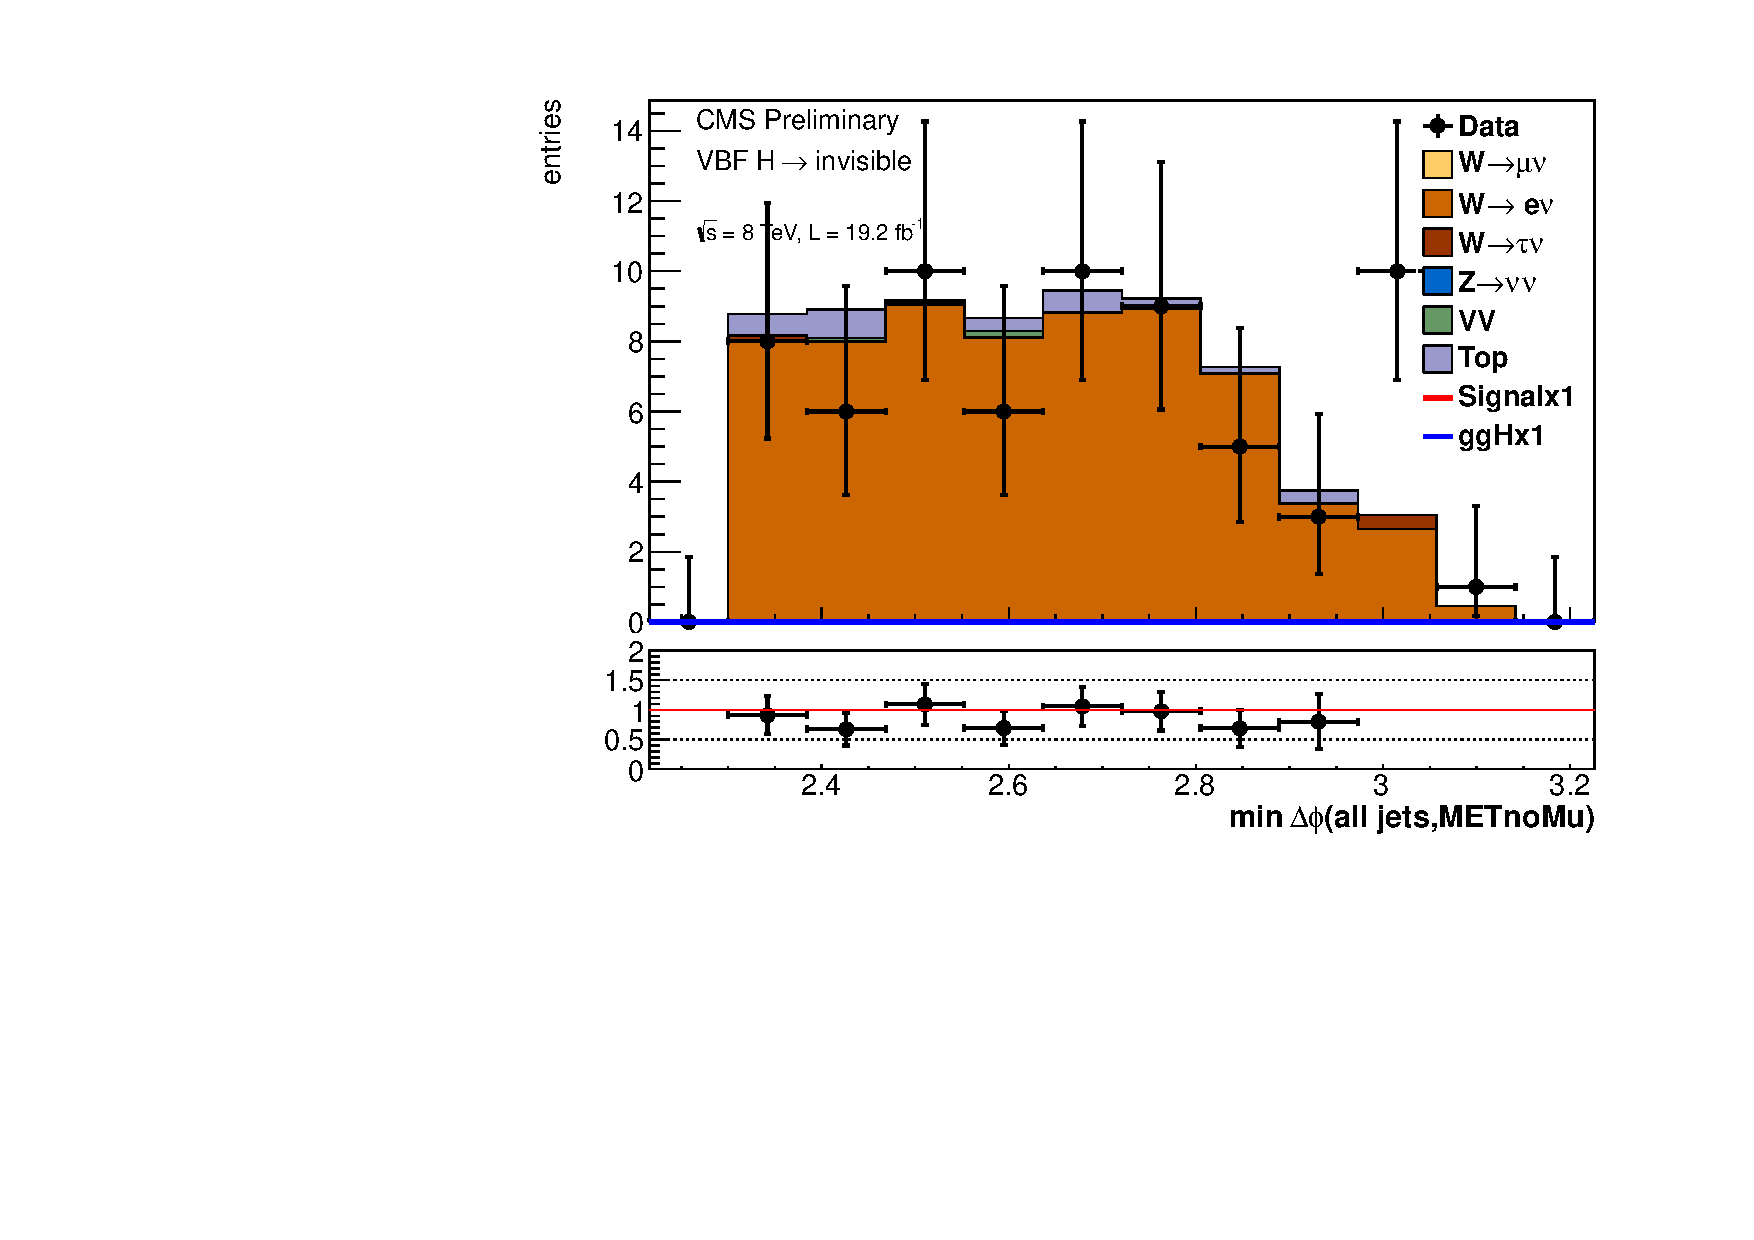
\includegraphics[width=.55\largefigwidth]{plots/parked/AN-14-243-figs/output_sigreg/enu_alljetsmetnomu_mindphi.pdf}}

  \caption{Distributions of variables in data and \ac{MC} events in the $\PW\rightarrow e\nu$ control region. \ac{MC} events from V+jets backgrounds are scaled by their data-driven scale factors. The variables shown are from top to bottom and left to right \detajj, \Mjj, the leading and subleading jet's \pt, \METnoMU, \METsig and \jetmetdphi.}
  \label{fig:parkedwenu}
\end{figure}

\subsection{W$\rightarrow \mu\nu$+jets}%??                                                                                                                  
\label{sec:parkedwmunu}
As for the $\PW\rightarrow e\nu$ background the $W\rightarrow \mu\nu$ background is estimated using \EquationRef{eq:wdatabkgrep} with a control region enriched in $\PW\rightarrow\mu\nu$ events through a change in lepton requirements. The control region used has the same requirements as the signal region, but with the muon veto replaced with a requirement that there is one tight muon and no other muons present in the event. The distributions of several variables in data and \ac{MC} (which has been scaled by the data driven scale factor extracted from this control region) are shown in \FigureRef{fig:parkedwmunu}, where good agreement can be seen. A table of the inputs to \EquationRef{eq:wdatabkgrep} can be seen in \TableRef{tab:parkedwmunu}. The contribution from other backgrounds in the $\PW\rightarrow\mu\nu$ control region is approximately 5\%. Again the scale factor obtained  for this background is significantly different from 1, being 0.71, and further investigation of this is detailed in \SectionRef{sec:parkedscalefactors}. Furthermore, the estimated contribution from this background is very different to that expected from $\PW\rightarrow e\nu$, an investigation of this difference is described in \SectionRef{sec:parkedenumunudiff}.

\begin{figure}
  \subfloat[]{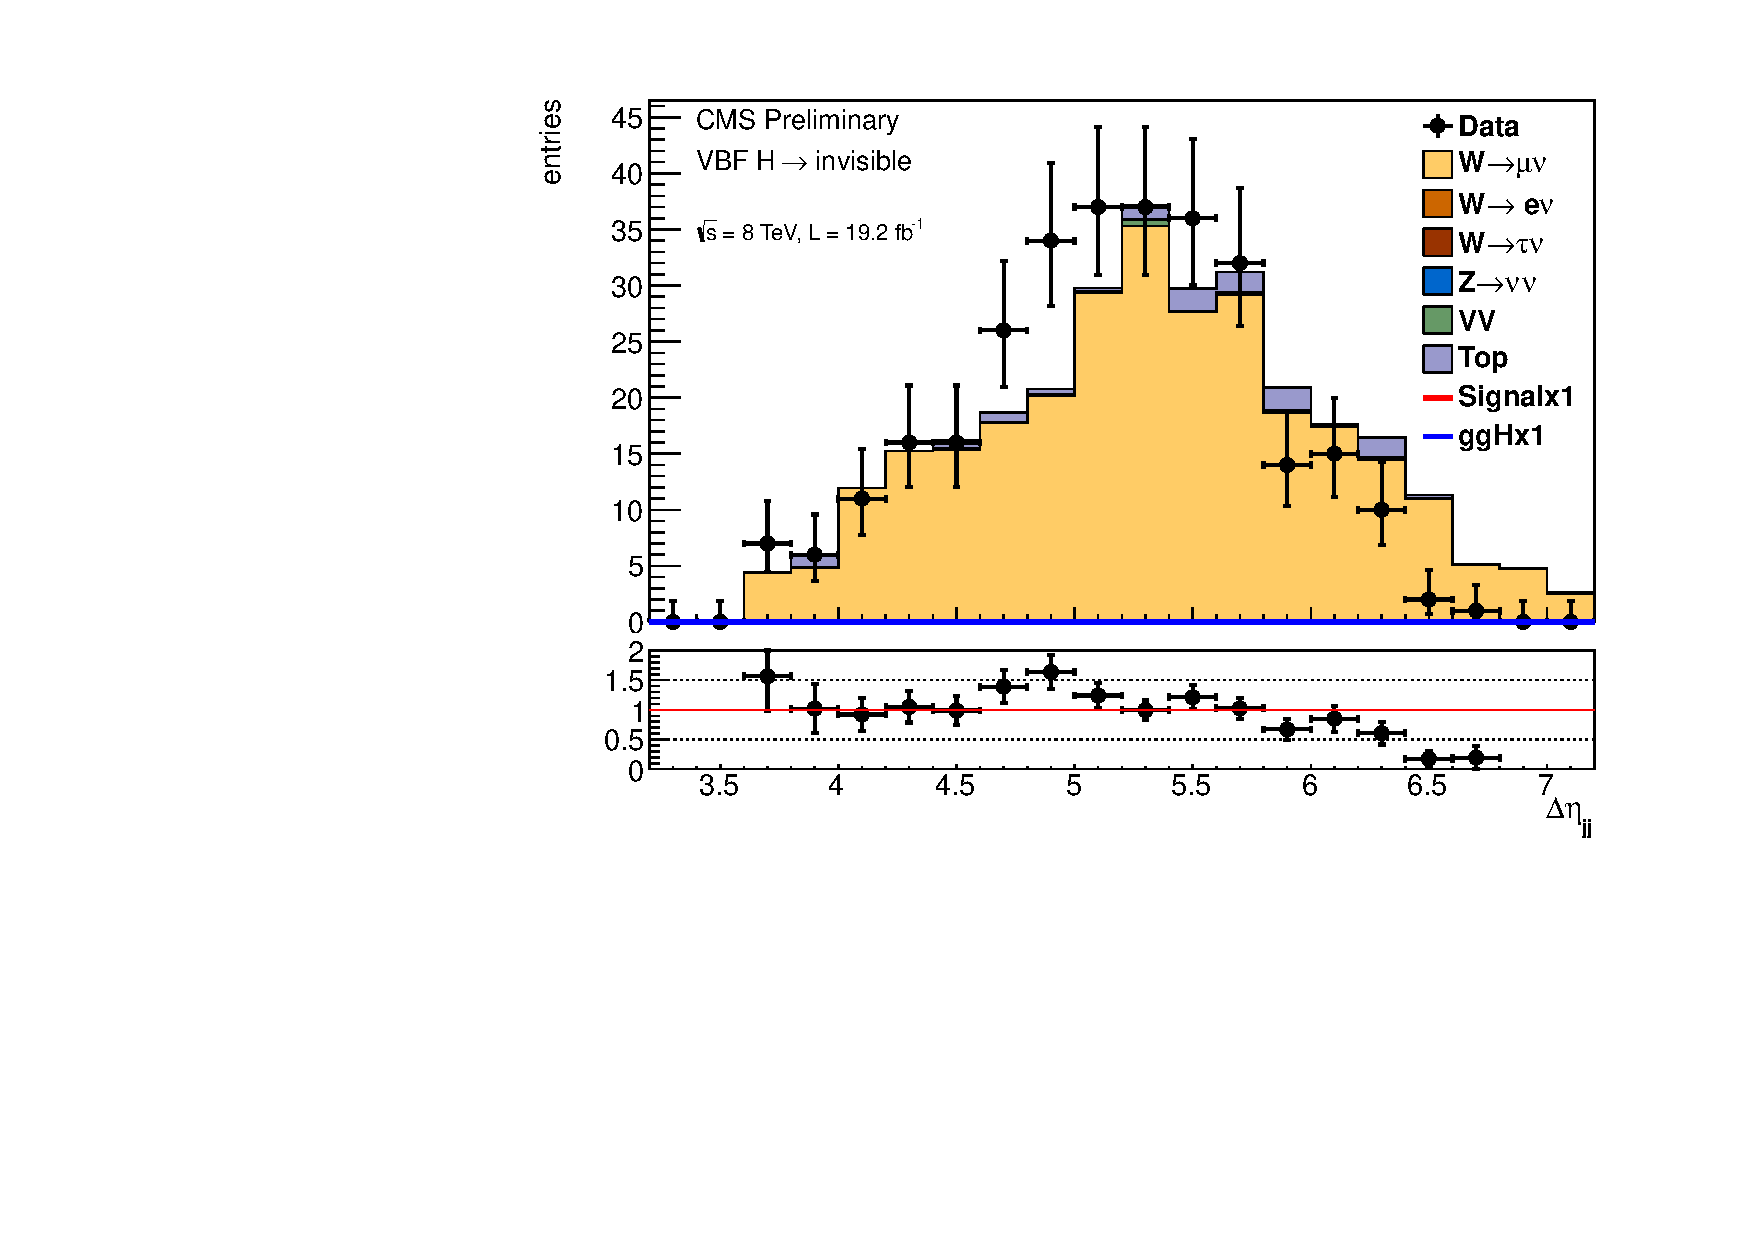
\includegraphics[width=.55\largefigwidth]{plots/parked/AN-14-243-figs/output_sigreg/munu_dijet_deta.pdf}}
  \subfloat[]{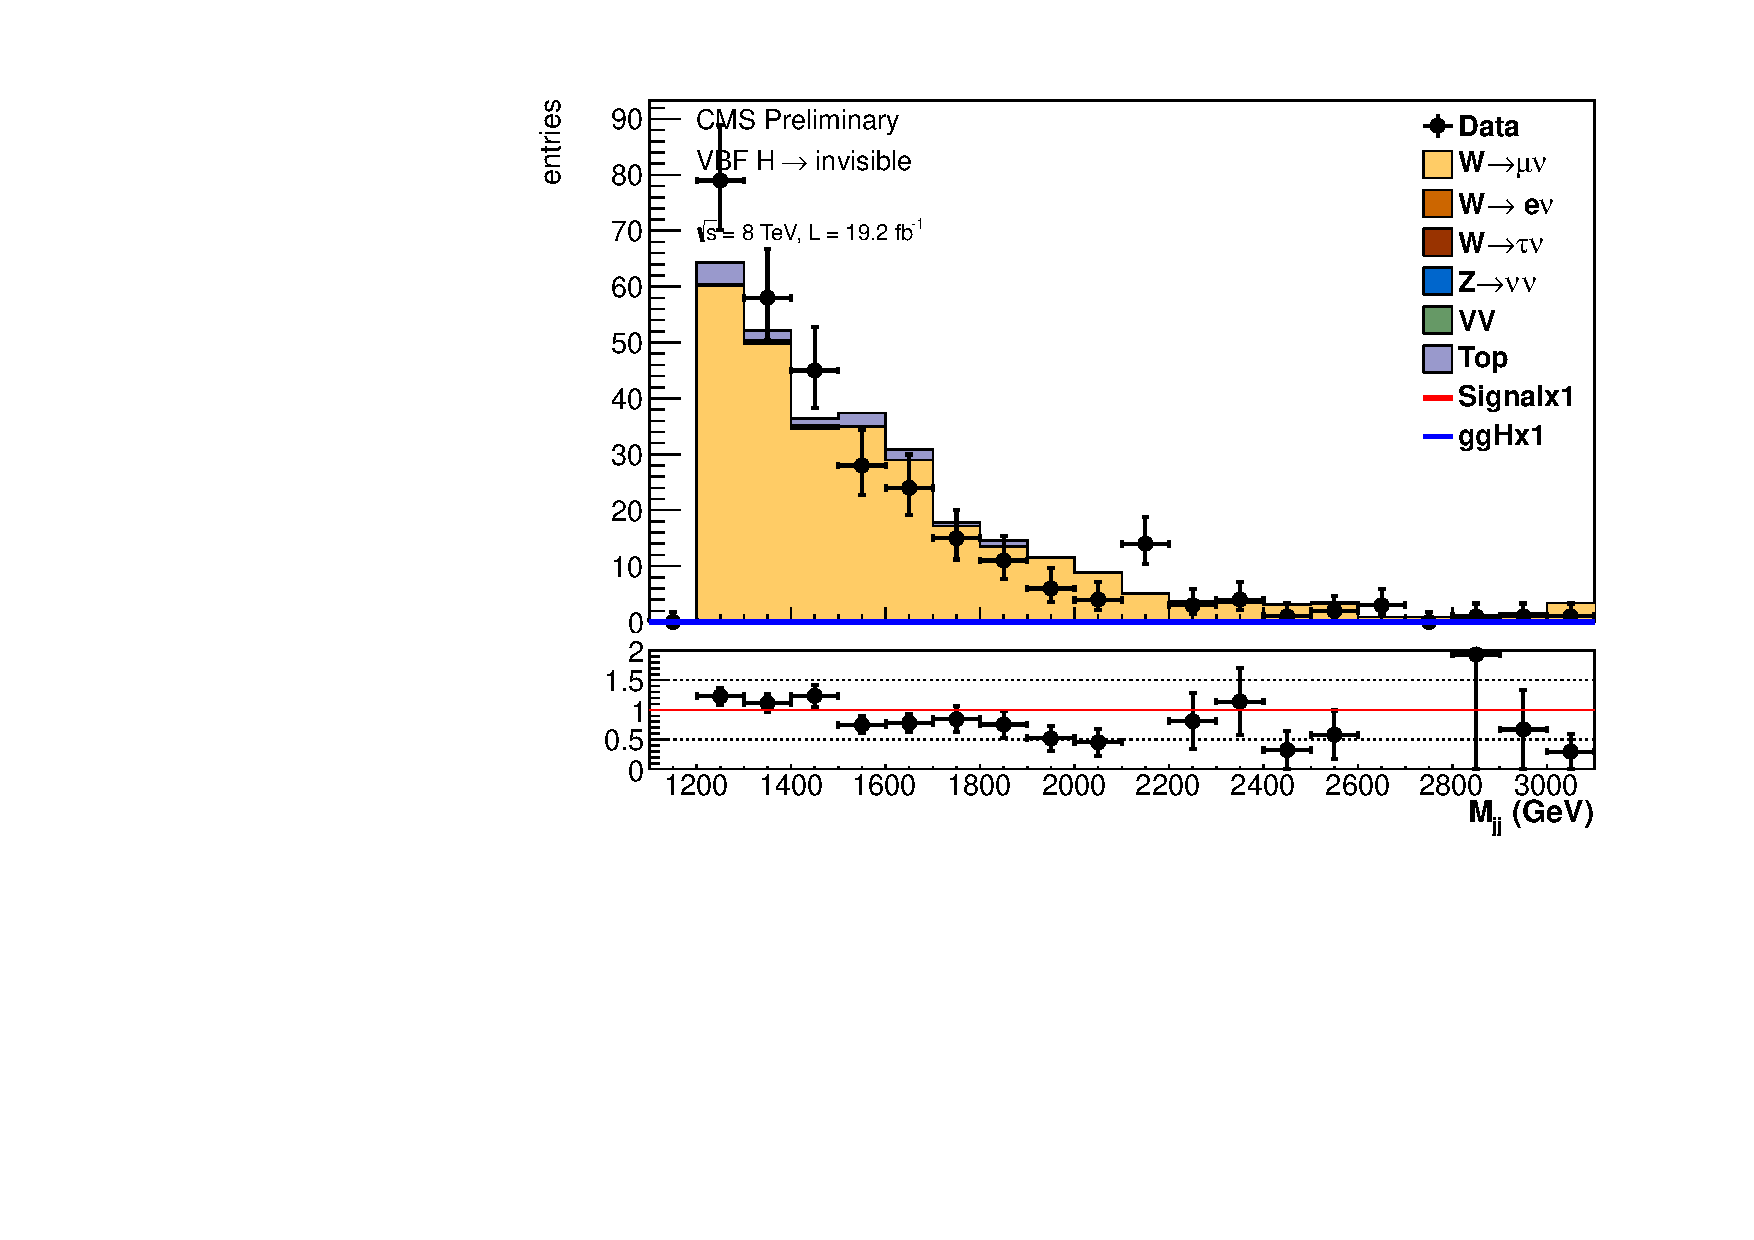
\includegraphics[width=.55\largefigwidth]{plots/parked/AN-14-243-figs/output_sigreg/munu_dijet_M.pdf}}

  \subfloat[]{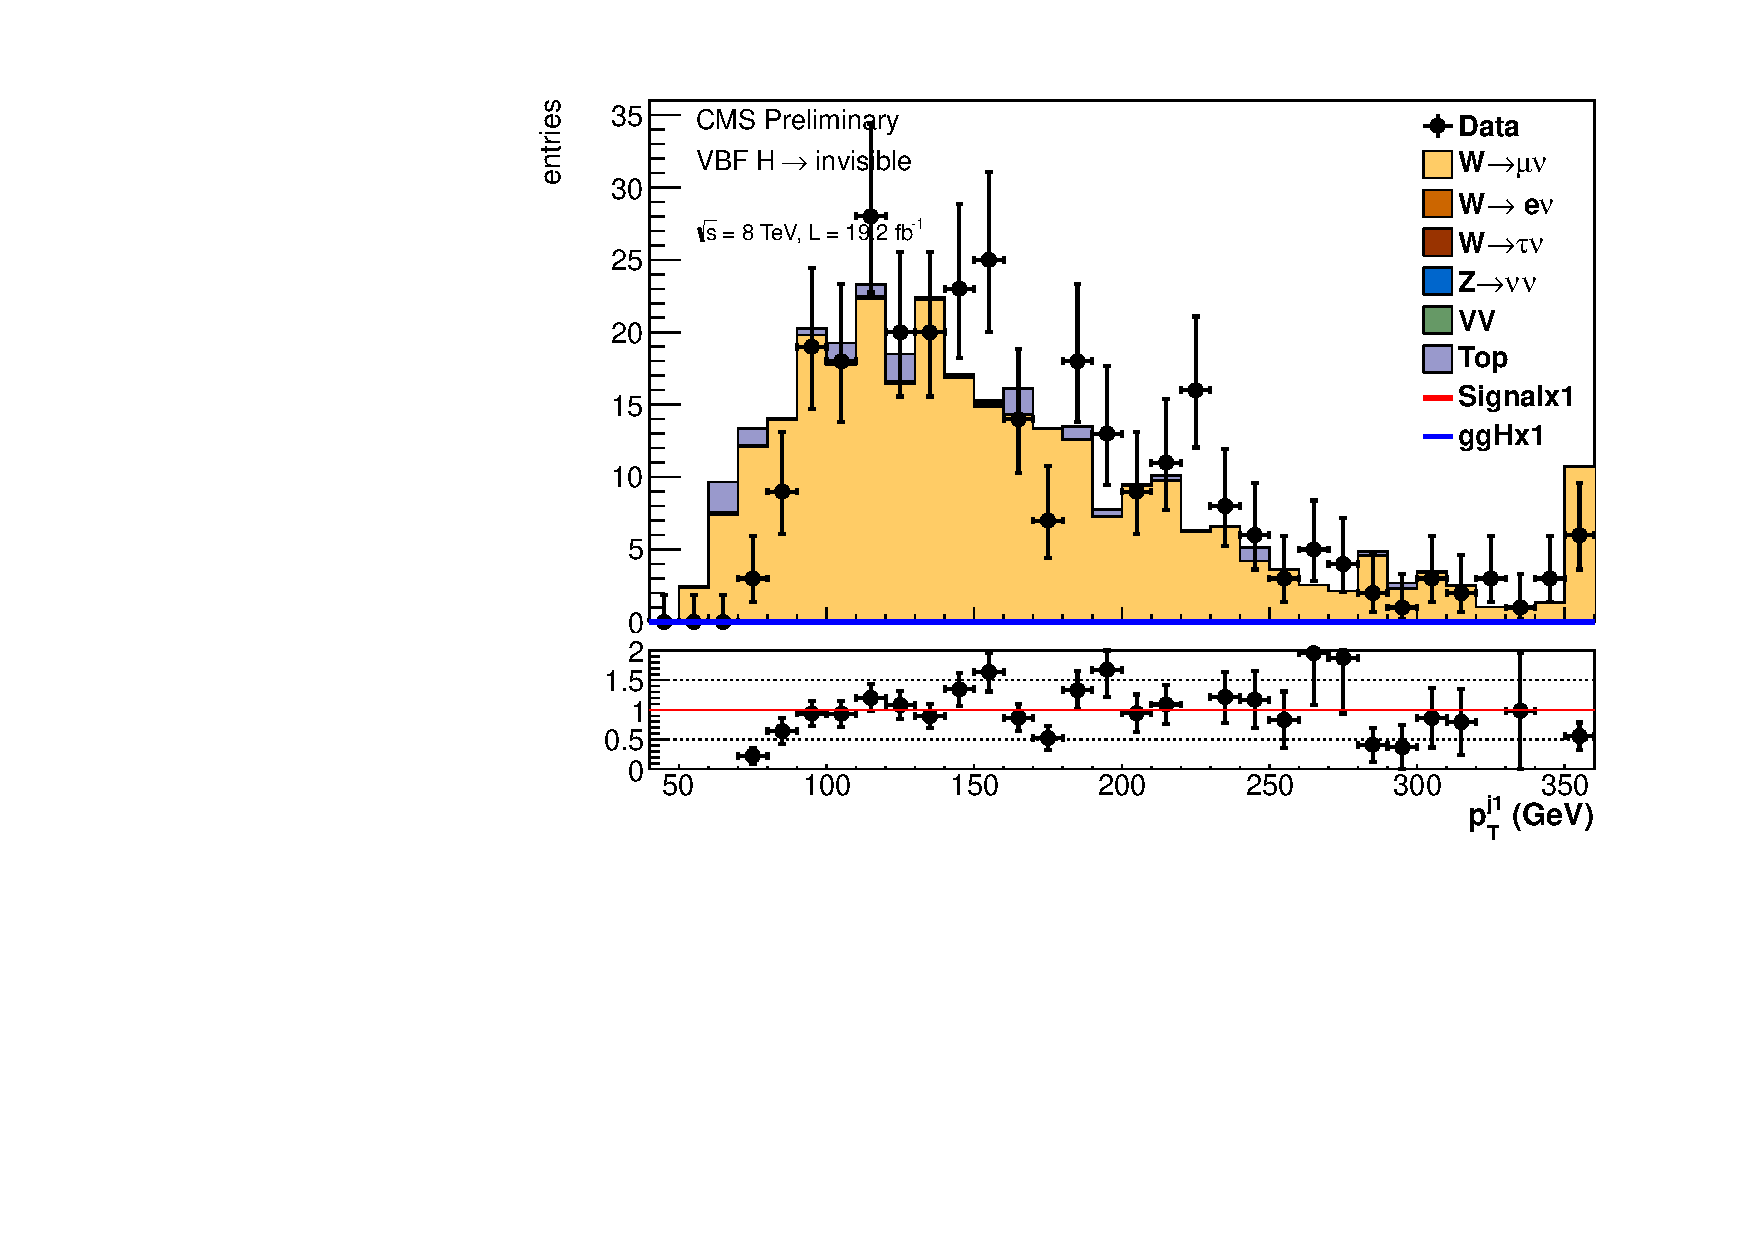
\includegraphics[width=.55\largefigwidth]{plots/parked/AN-14-243-figs/output_sigreg/munu_jet1_pt.pdf}}
  \subfloat[]{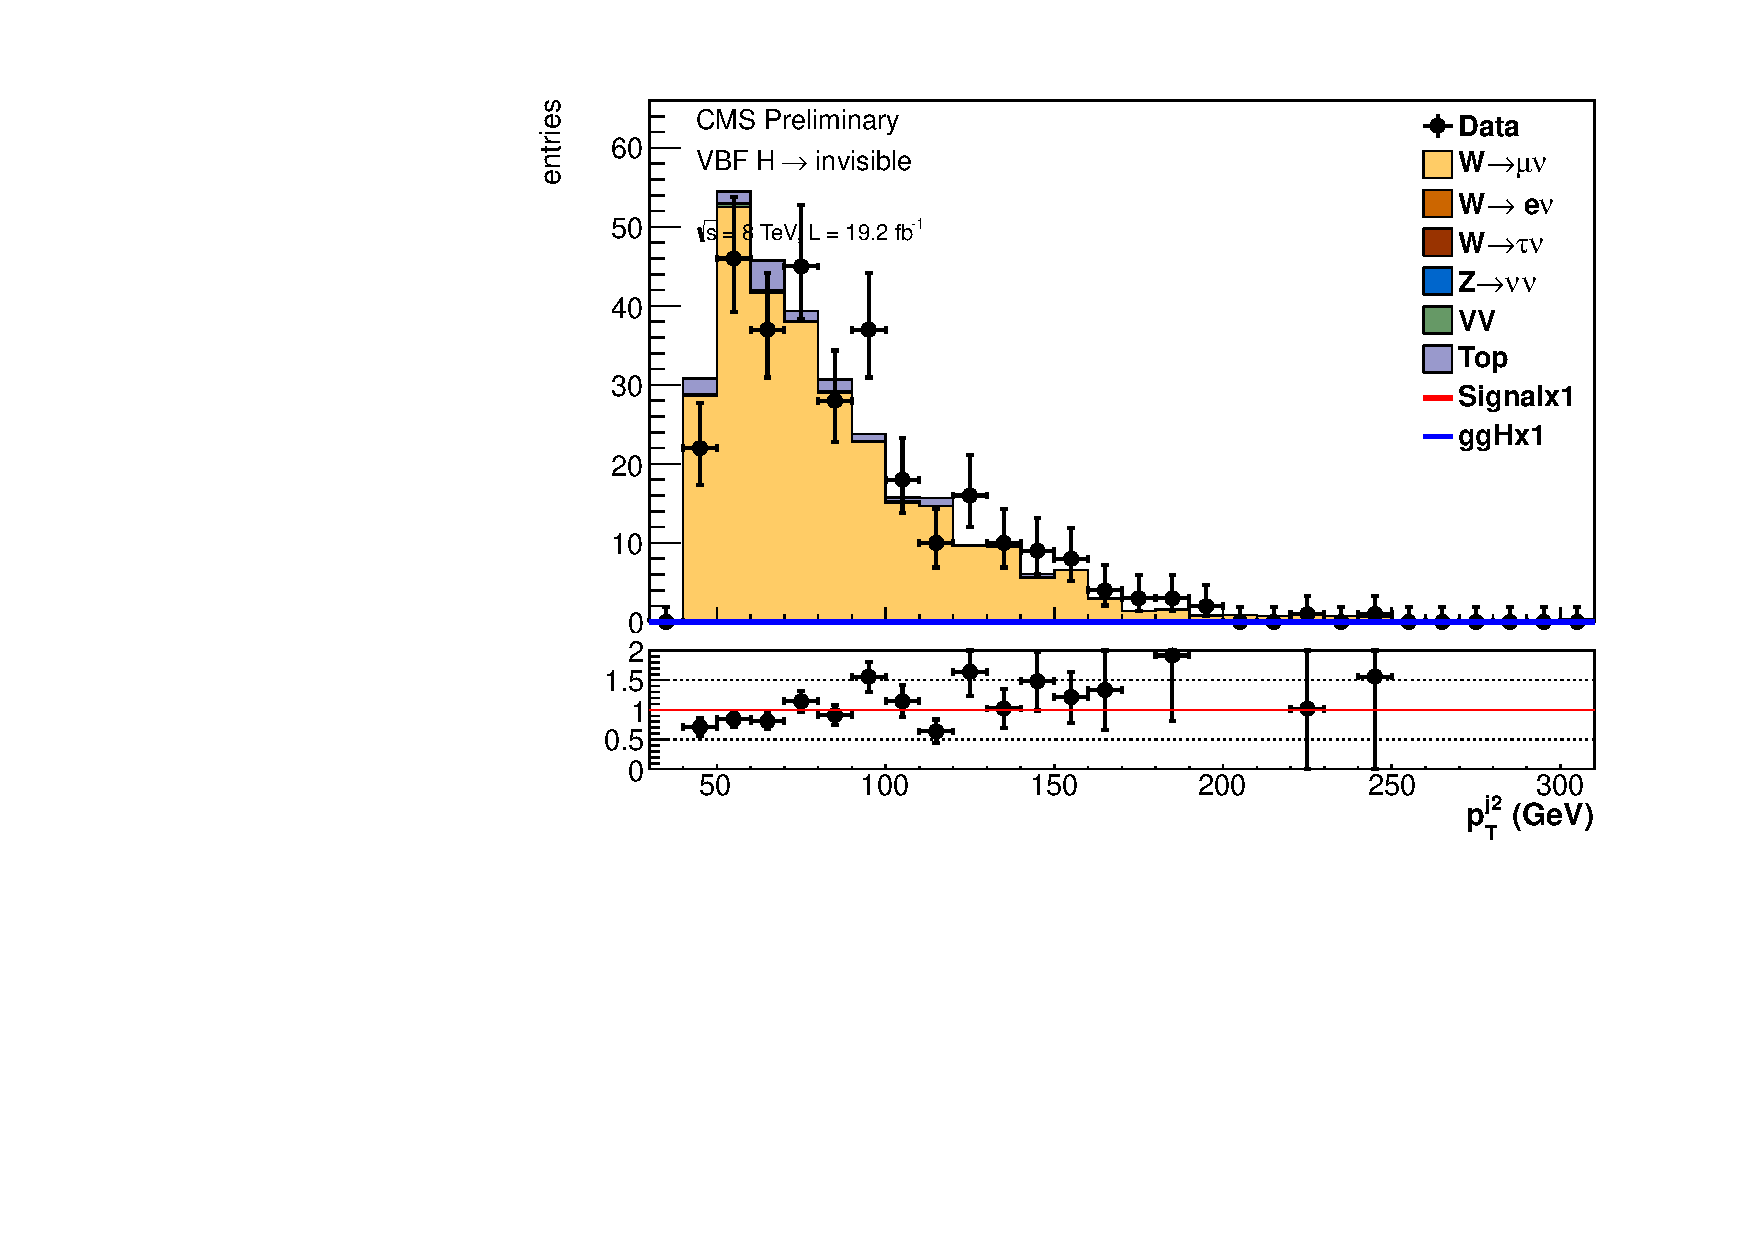
\includegraphics[width=.55\largefigwidth]{plots/parked/AN-14-243-figs/output_sigreg/munu_jet2_pt.pdf}}

  \subfloat[]{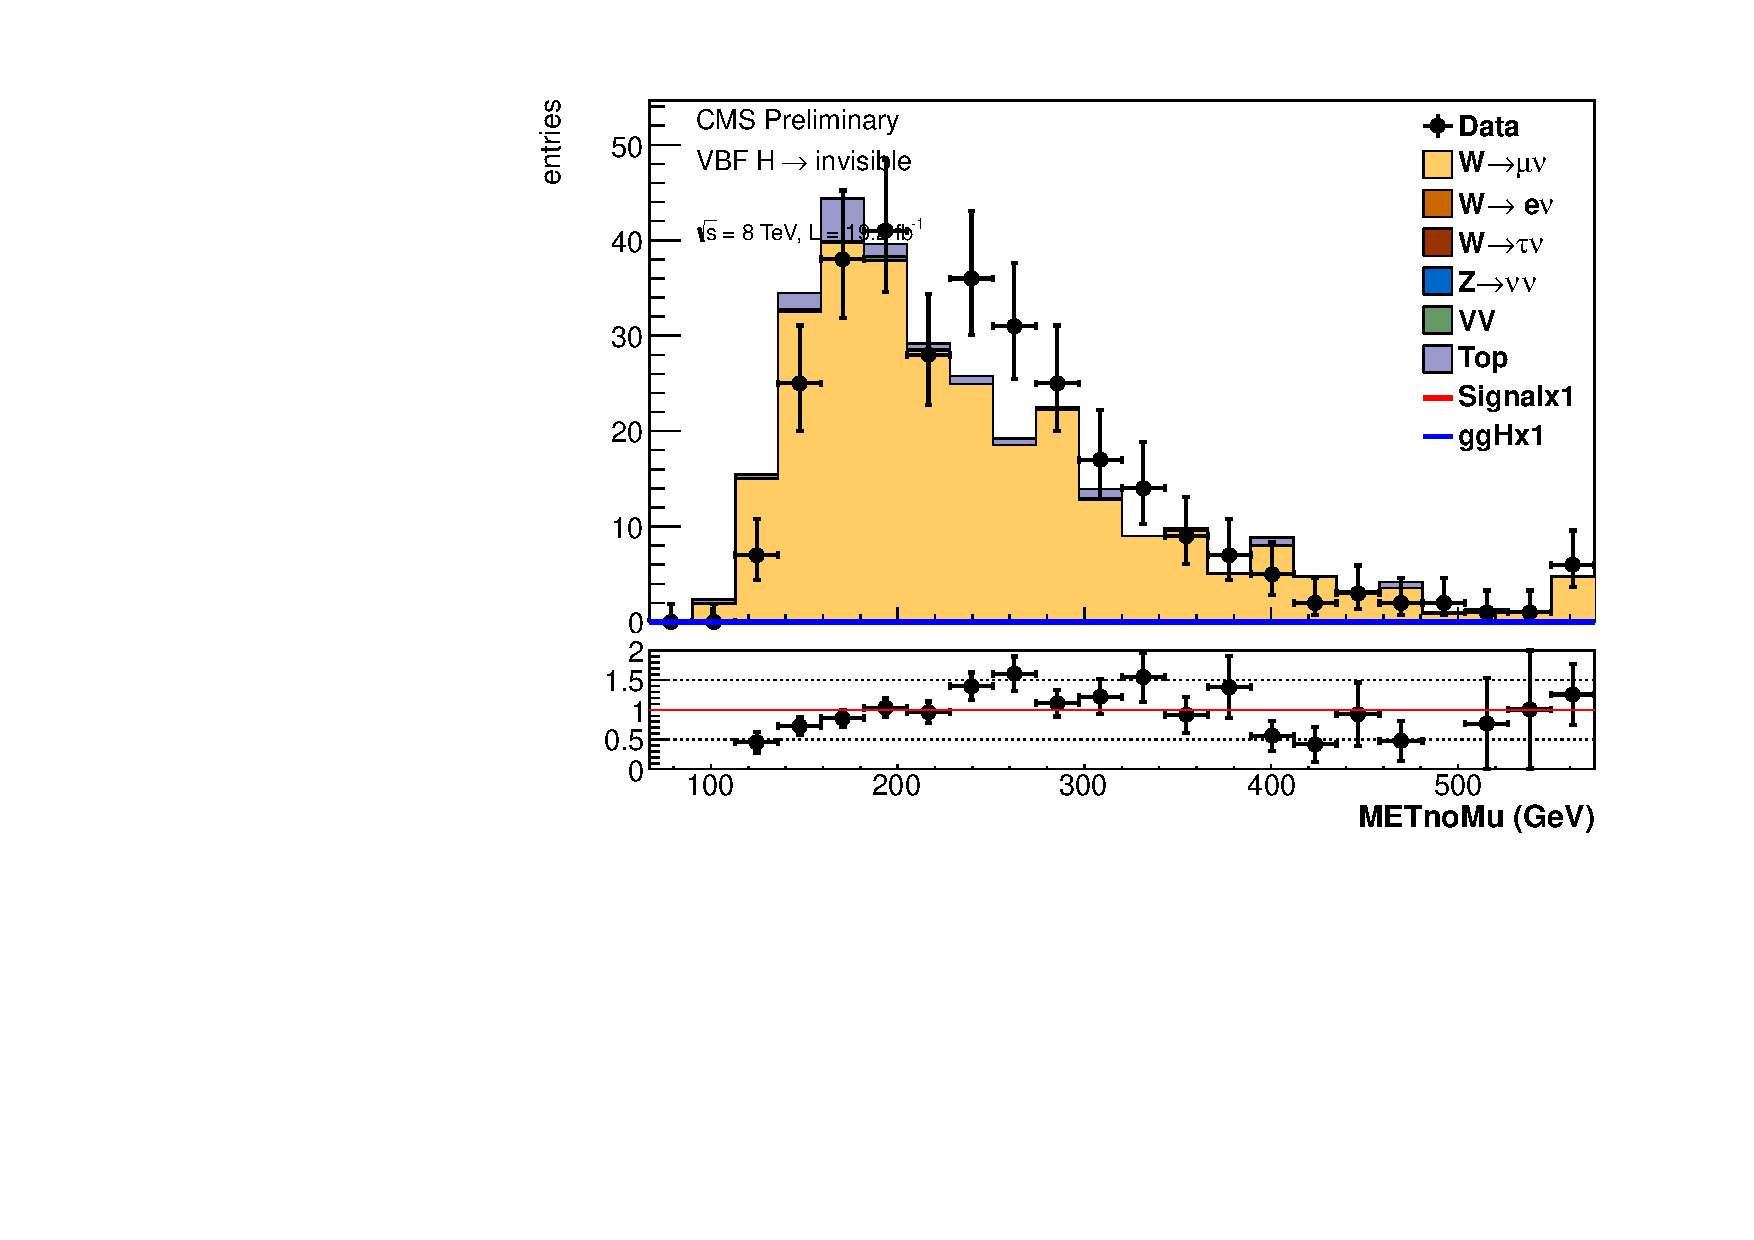
\includegraphics[width=.55\largefigwidth]{plots/parked/AN-14-243-figs/output_sigreg/munu_metnomuons.pdf}}
  \subfloat[]{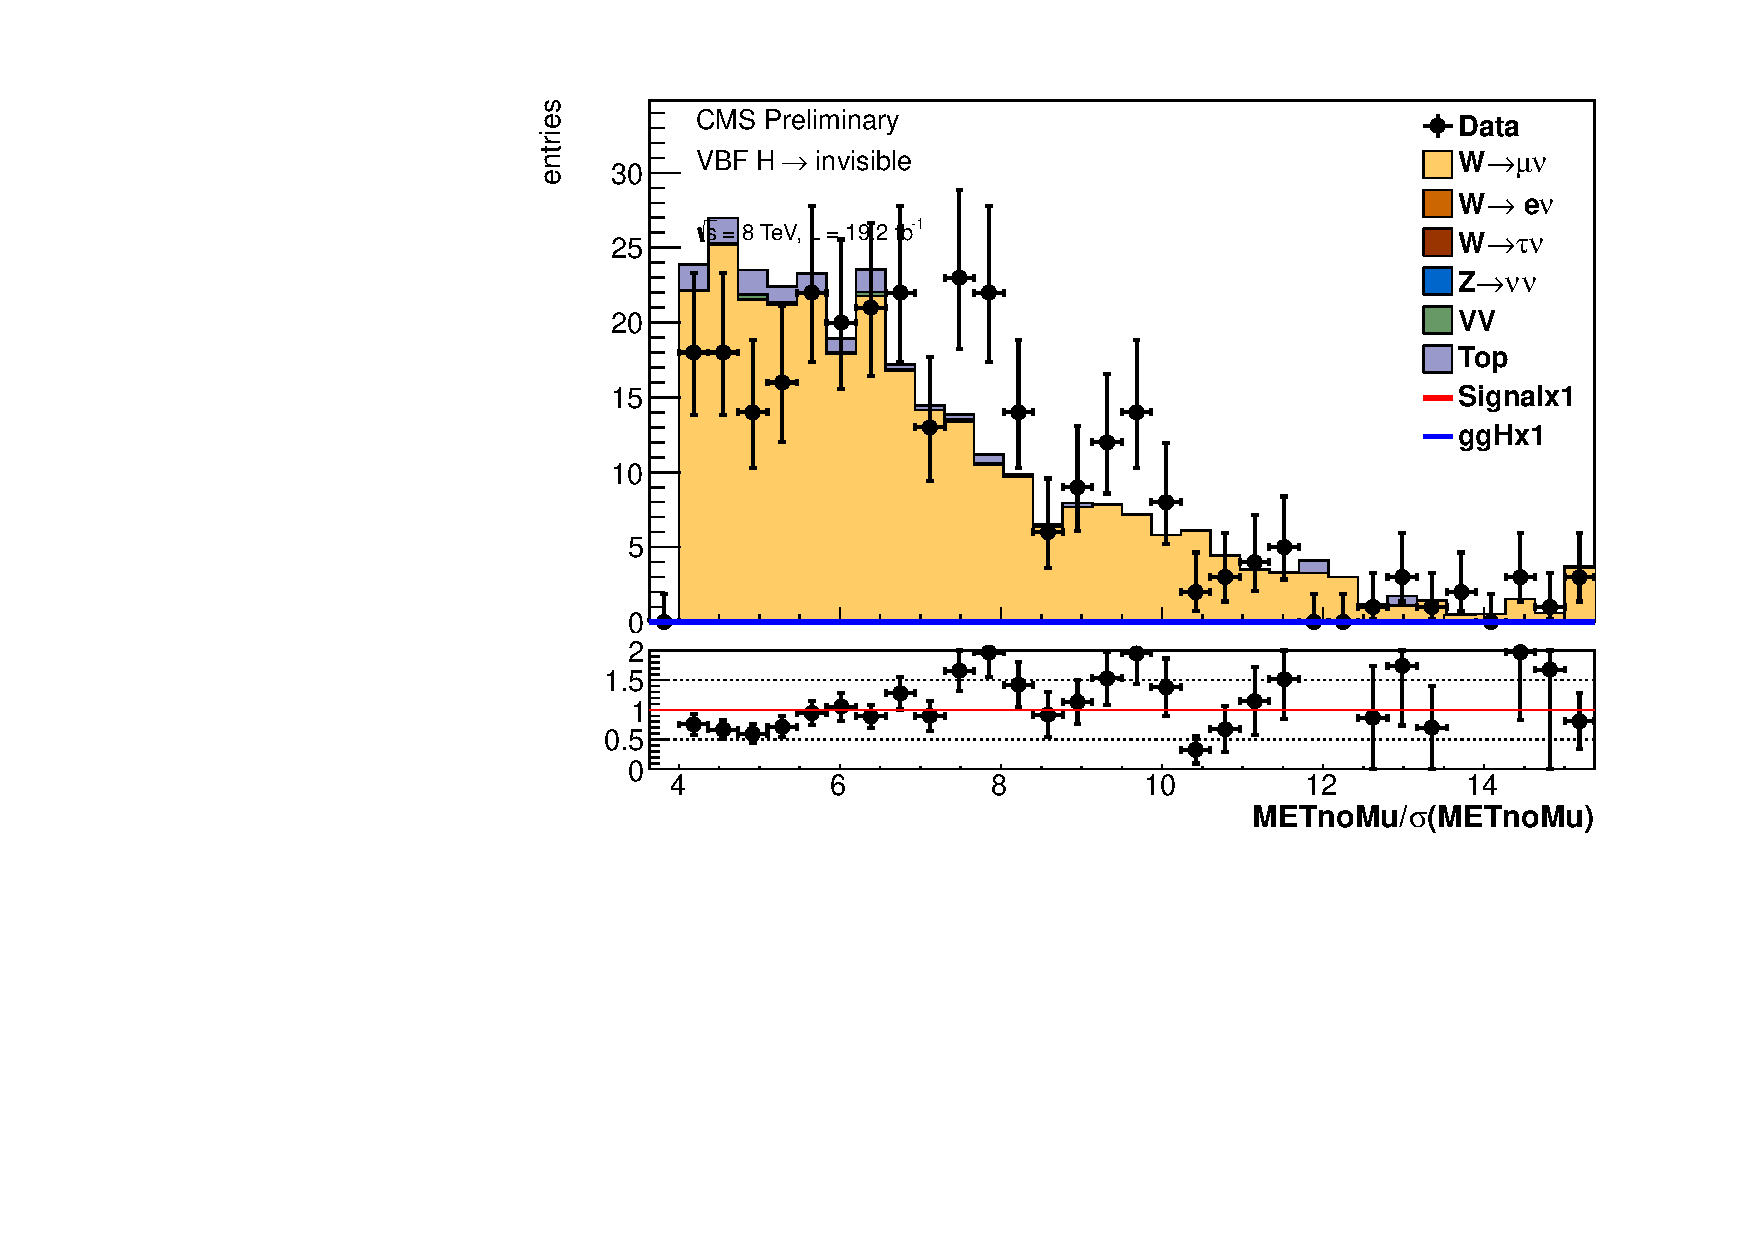
\includegraphics[width=.55\largefigwidth]{plots/parked/AN-14-243-figs/output_sigreg/munu_metnomu_significance.pdf}}

  \subfloat[]{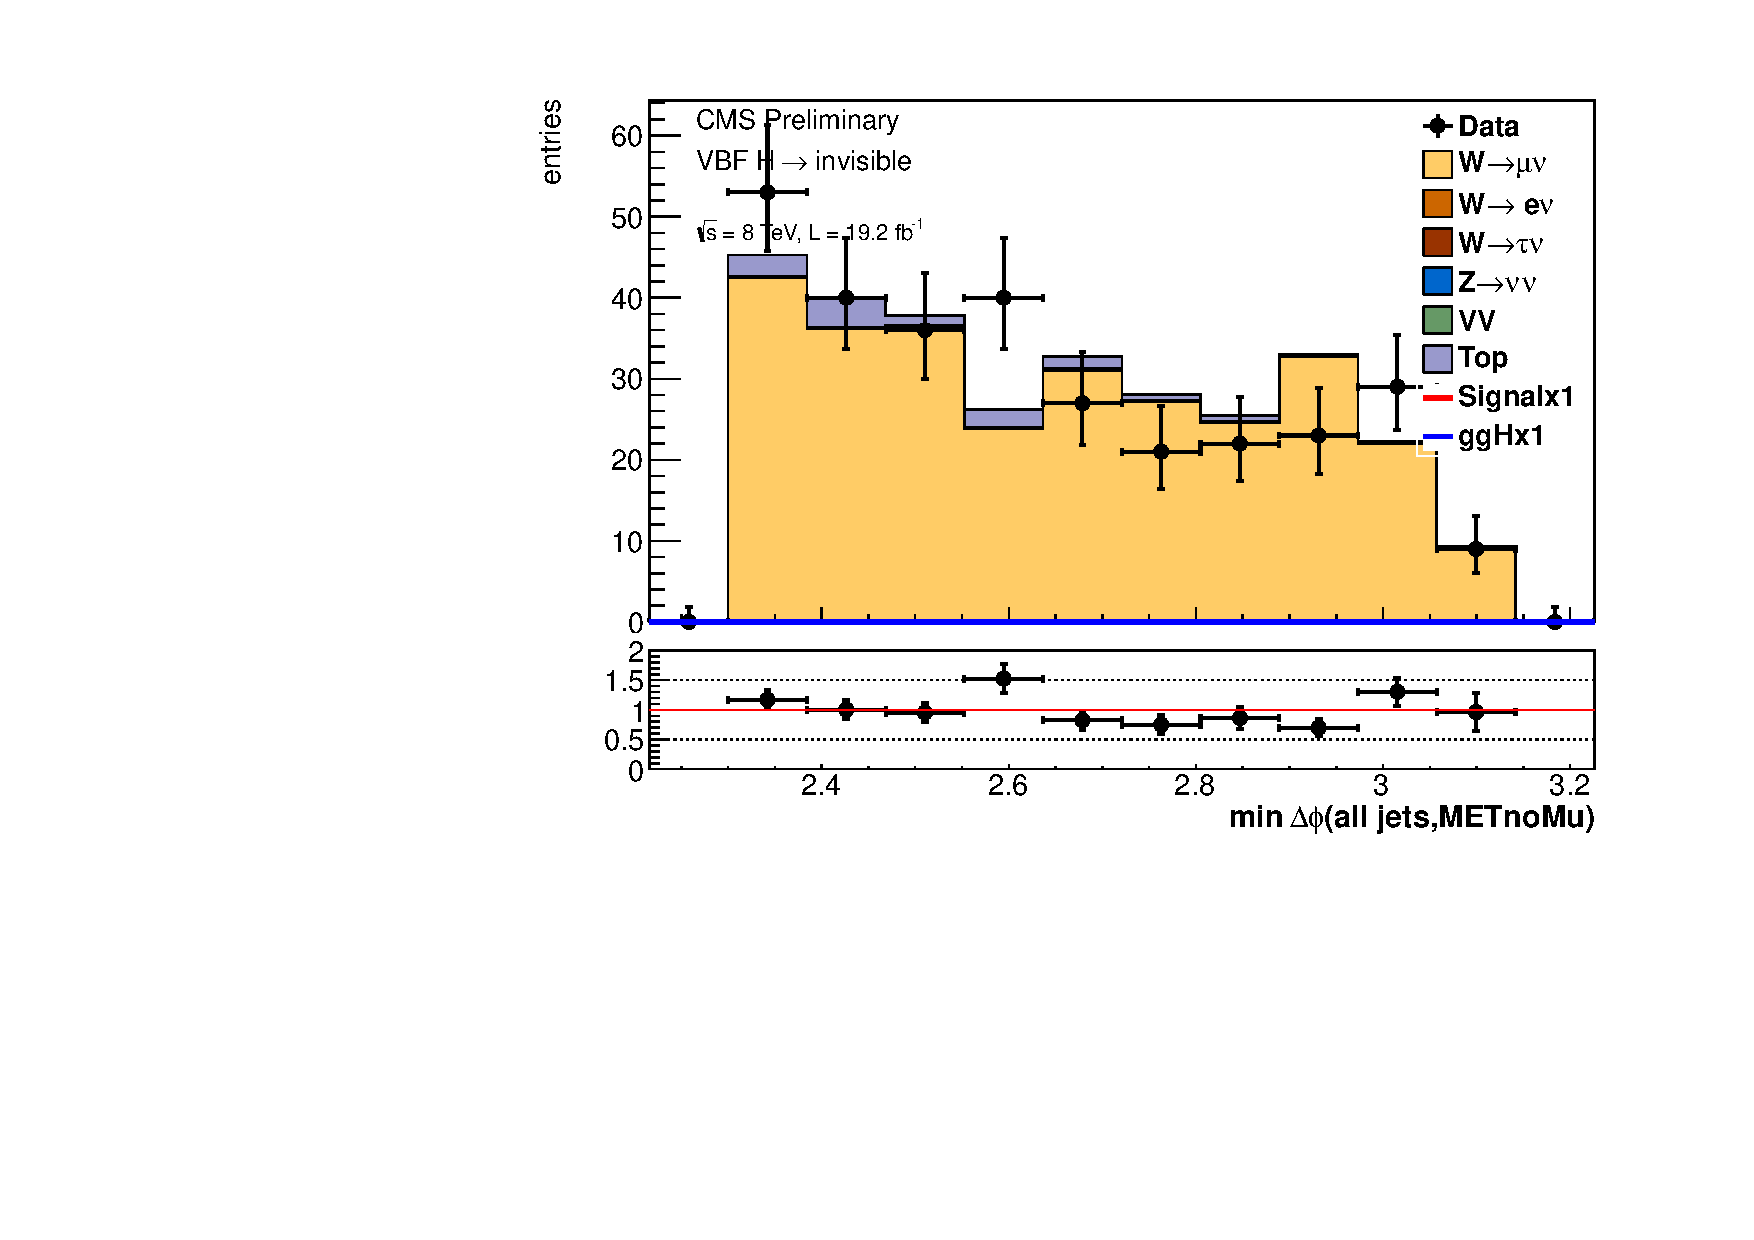
\includegraphics[width=.55\largefigwidth]{plots/parked/AN-14-243-figs/output_sigreg/munu_alljetsmetnomu_mindphi.pdf}}
    \caption{Distributions of variables in data and \ac{MC} events in the $\PW\rightarrow \mu\nu$ control region. \ac{MC} events from V+jets backgrounds are scaled by their data-driven scale factors. The variables shown are from top to bottom and left to right \detajj, \Mjj, the leading and subleading jet's \pt, \METnoMU, \METsig and \jetmetdphi.}
  \label{fig:parkedwmunu}
\end{figure}

\begin{table}[h!]
  \begin{center}
    \caption{The inputs to and results of \EquationRef{eq:wdatabkgrep}, when used to estimate the $W\rightarrow \mu\nu$ estimate in the signal
      region.}
    \label{tab:parkedwmunu}
    \begin{tabular}{lcc}
      \hline
      \hline
      & Signal region & Control region \\
      \hline
      \hline
      $N_{Data}$&N/A&$300\pm 17.3$\stat\\
      $N_{Bkg}$&N/A&$14.8\pm 2.5(MC stat)$\\
      $N_{MC}$&$143.7\pm10.2(MC stat)$&$399.9\pm 14.9(MC stat)$\\
      \hline
      $\frac{N^{data}-N^{bkg}}{N^{MC}_{C}}$ & \multicolumn{2}{c|}{$0.71\pm0.04$\stat$\pm0.03$(MC stat.)} \\
      \hline
      $N_{\PW\rightarrow\mu\nu}$&\textcolor{red}{$102.5\pm6.2$\stat$\pm11.7$\syst}&N/A \\
      \hline
      \hline
    \end{tabular}
  \end{center}
\end{table}



\subsection{W$\rightarrow \tau\nu$+jets}%??                                                                                                                 
\label{sec:parkedwtaunu}
%??region
The signal region requirements do not include a veto of hadronic taus, due to the low identification efficiency and relatively high probability for a jet to be identified as a fake tau. Requiring that there is an identified hadronic tau in addition to the signal region selection results in a region containing only 2 data events. In order to increase the number of events in the tau control region the \jetmetdphi cut was removed. Whilst the requirement that there is an identified tau reduces the \ac{QCD} multijet contribution in the low \jetmetdphi region significantly compared to what was seen during the choice of the preselection. However, poor data-\ac{MC} agreement was still observed in the \jetmetdphi<1 region, which is evidence that some events from multijet processes are still present. To remove these \ac{QCD} multijet events, whilst keeping a reasonable number of events in the resulting control region, a requirement that \jetmetdphileading is greater than 1 and that the transverse mass of the hadronic tau and \MET system is greater than 20 \GeV. The \jetmetdphileading requirement reduces multijet backgrounds for the same reason that \jetmetdphi does, but it is a slightly looser requirement as it only considers the two leading jets. The transverse mass of the tau-\MET system is a good variable to reject \ac{QCD} where a lepton is present as in real \PW boson events the tau and \MET are expected to originate from the same object and therefore have significant invariant mass, which is not the case for \ac{QCD} multijet events.

After the anti-\ac{QCD} cuts the agreement between data and \ac{MC} is good as can be seen in \FigureRef{fig:parkedwtaunu} To account for the different \jetmetdphi selection in this region and the signal region the data driven scale factor was calculated both in the $\PW\rightarrow\mu\nu$ control region, which has the signal region \jetmetdphi selection, and in a modified single muon control region with the $\PW\rightarrow\tau\nu$ control region \jetmetdphi selection. The difference between these two scale factors was found to be 20\%, so a 20\% systematic uncertainty was added to the estimate of the $\PW\rightarrow\tau\nu$ background.

The single tau control region with a \jetmetdphileading cut and no \jetmetdphi cut was used with \EquationRef{eq:wdatabkgrep} to estimate the number of $\PW\rightarrow\tau\nu$ events in the signal region. A table of the inputs to \EquationRef{eq:wdatabkgrep} can be seen in \TableRef{tab:parkedwtaunu}. The contribution from other backgrounds in the $\PW\rightarrow\tau\nu$ control region is approximately 15\%, with most of these other background events being due to top quark related processes. The scale factor obtained for this background is 0.78, which is closer to 1 than those seen in the other \PW+jets backgrounds, however it also has the largest uncertainty. Further investigation of the V+jets scale factors is detailed in \SectionRef{sec:parkedscalefactors}.

\begin{figure}
  \subfloat[]{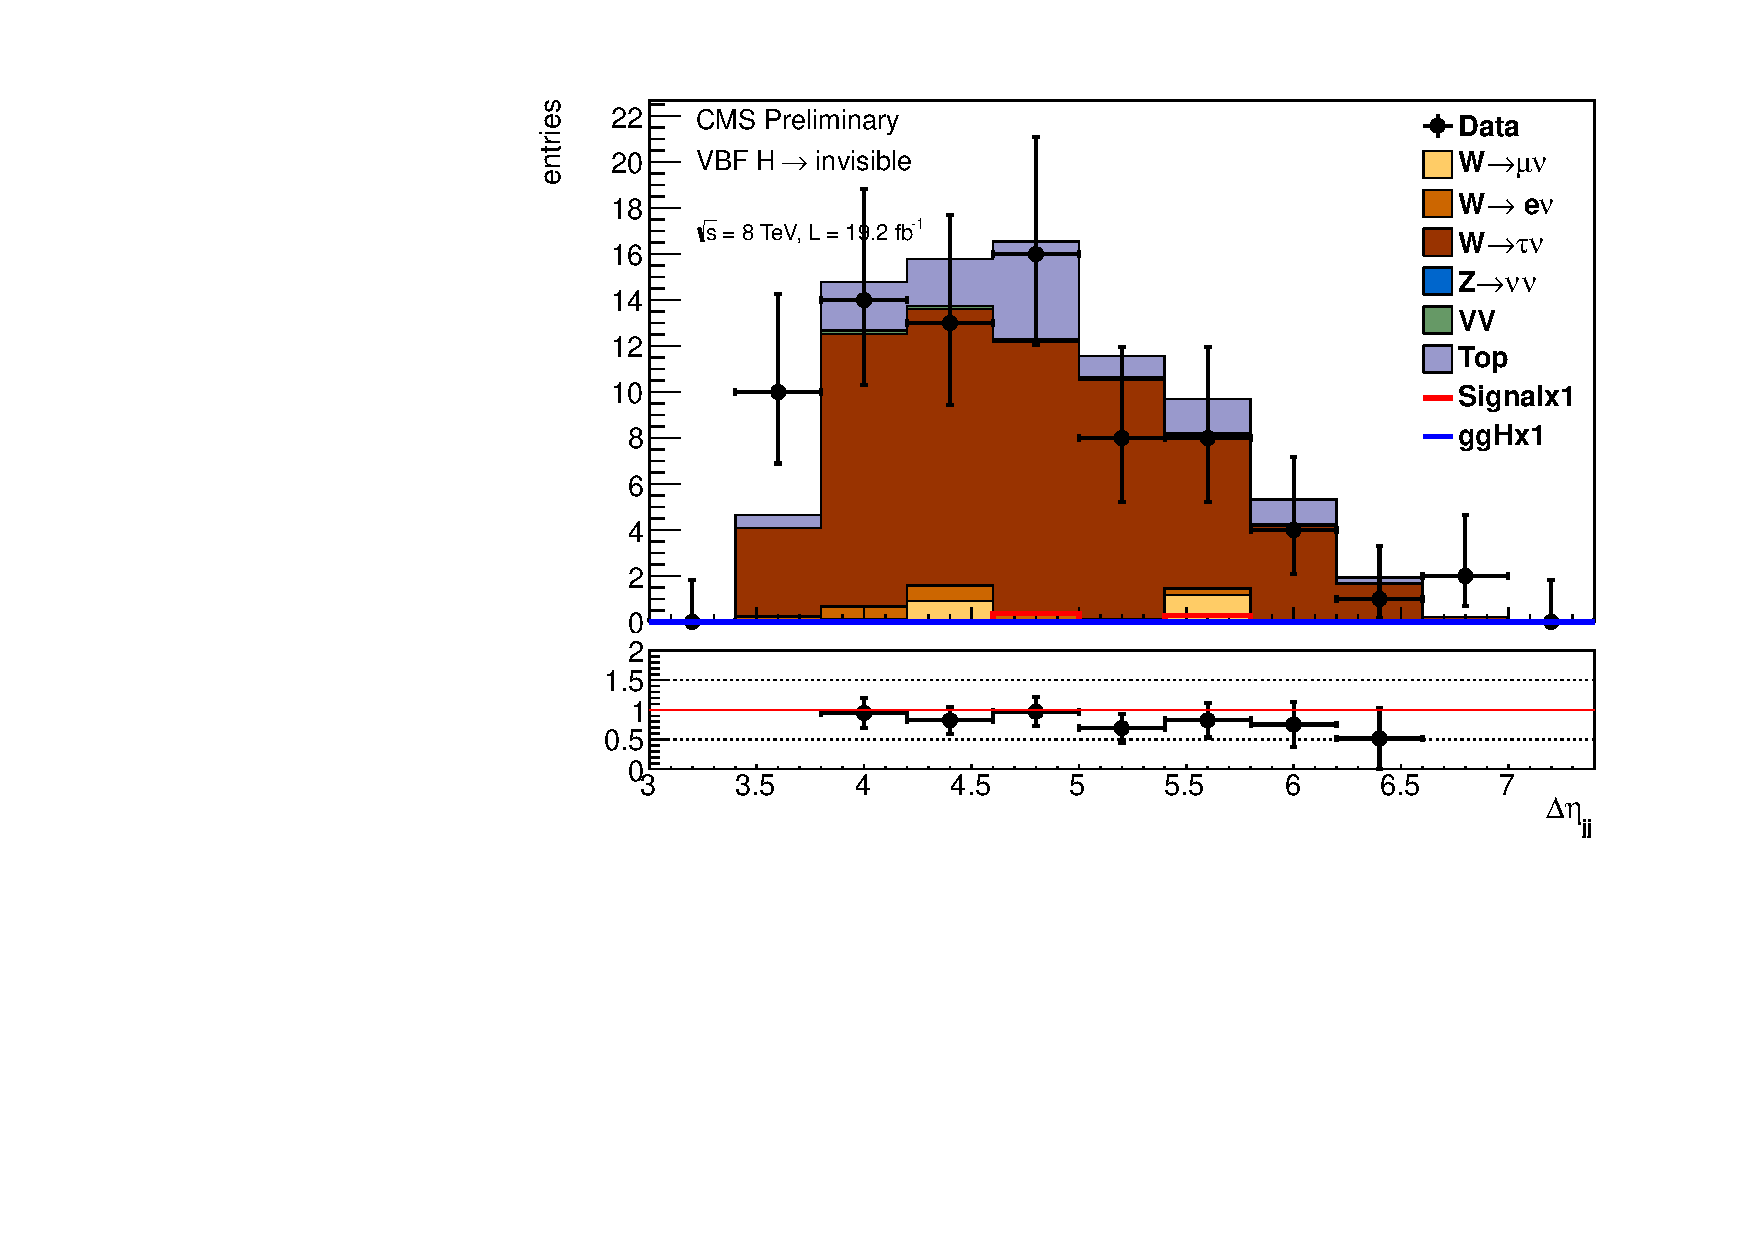
\includegraphics[width=.55\largefigwidth]{plots/parked/AN-14-243-figs/output_sigreg/taunu_dijet_deta.pdf}}
  \subfloat[]{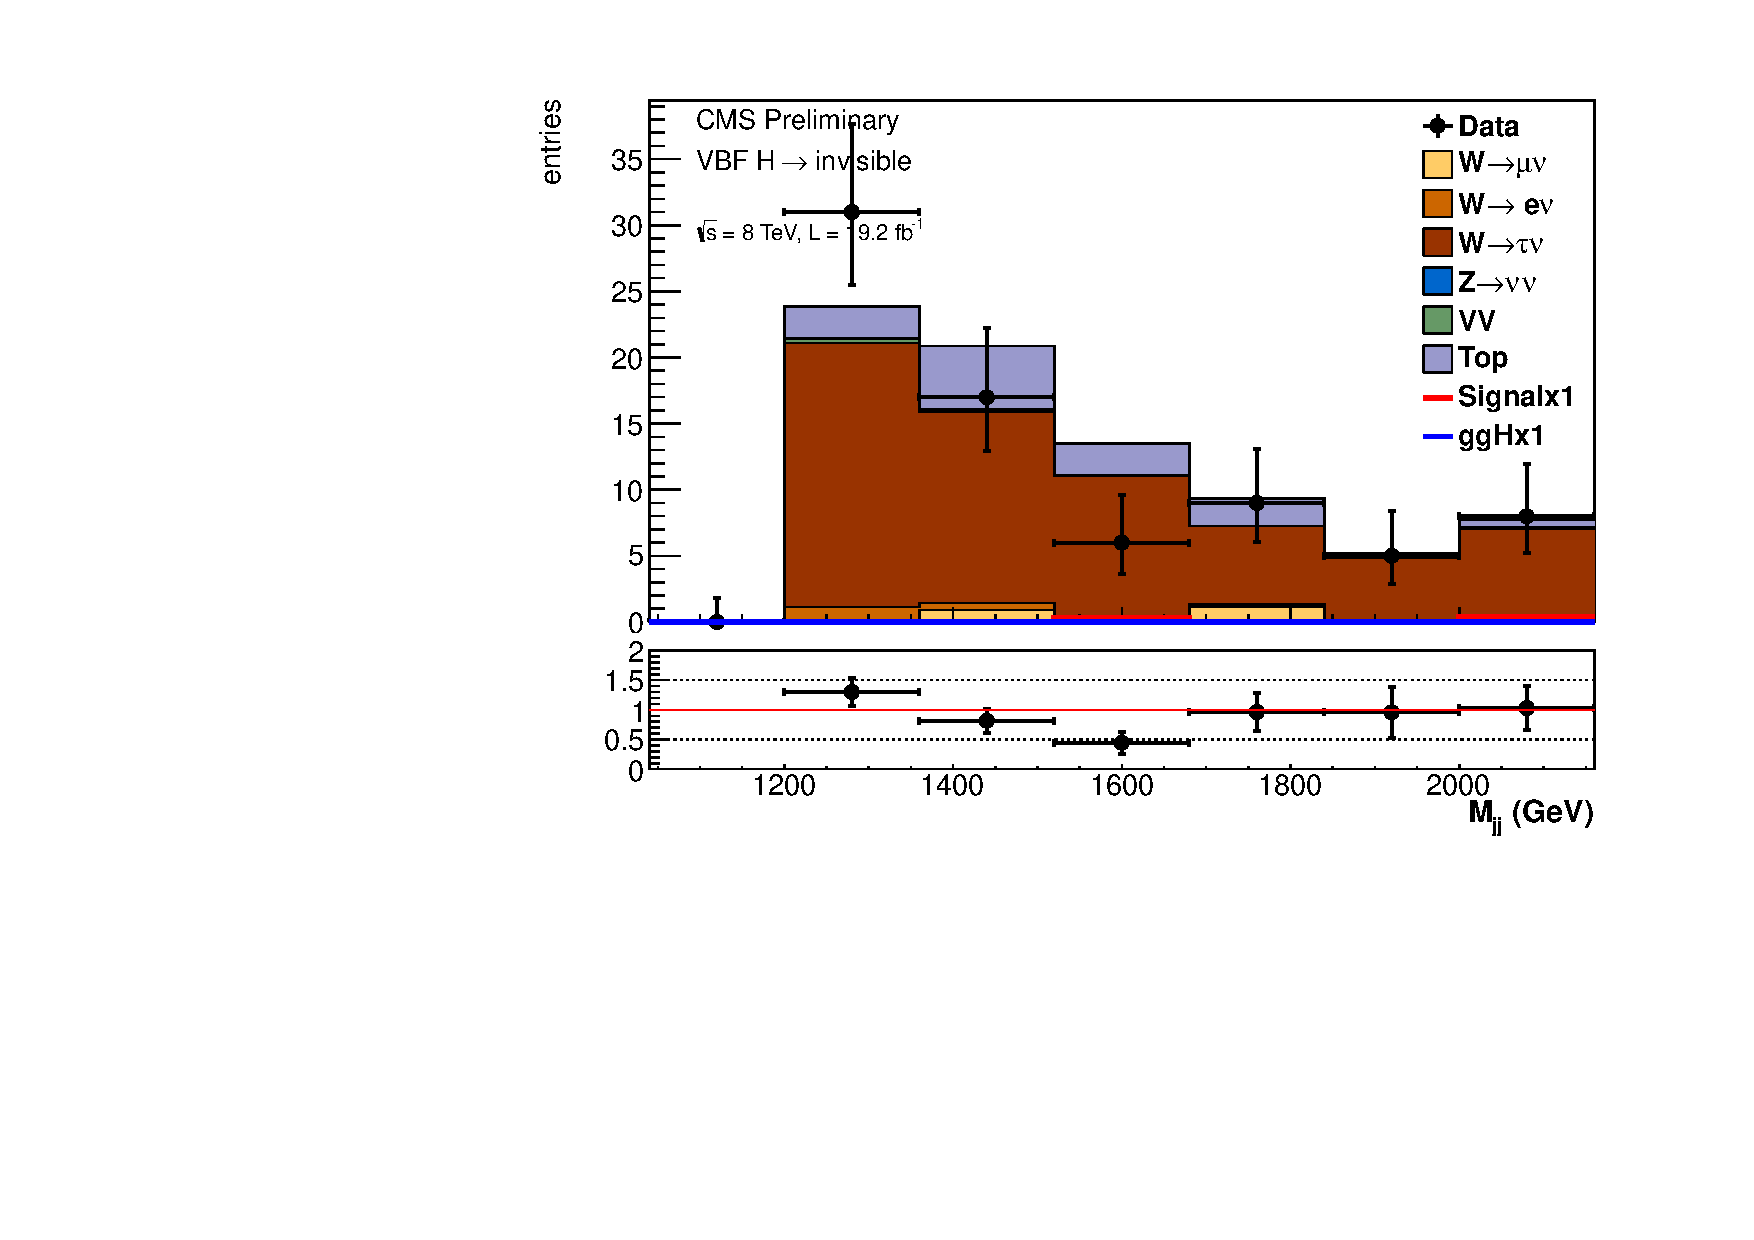
\includegraphics[width=.55\largefigwidth]{plots/parked/AN-14-243-figs/output_sigreg/taunu_dijet_M.pdf}}

  \subfloat[]{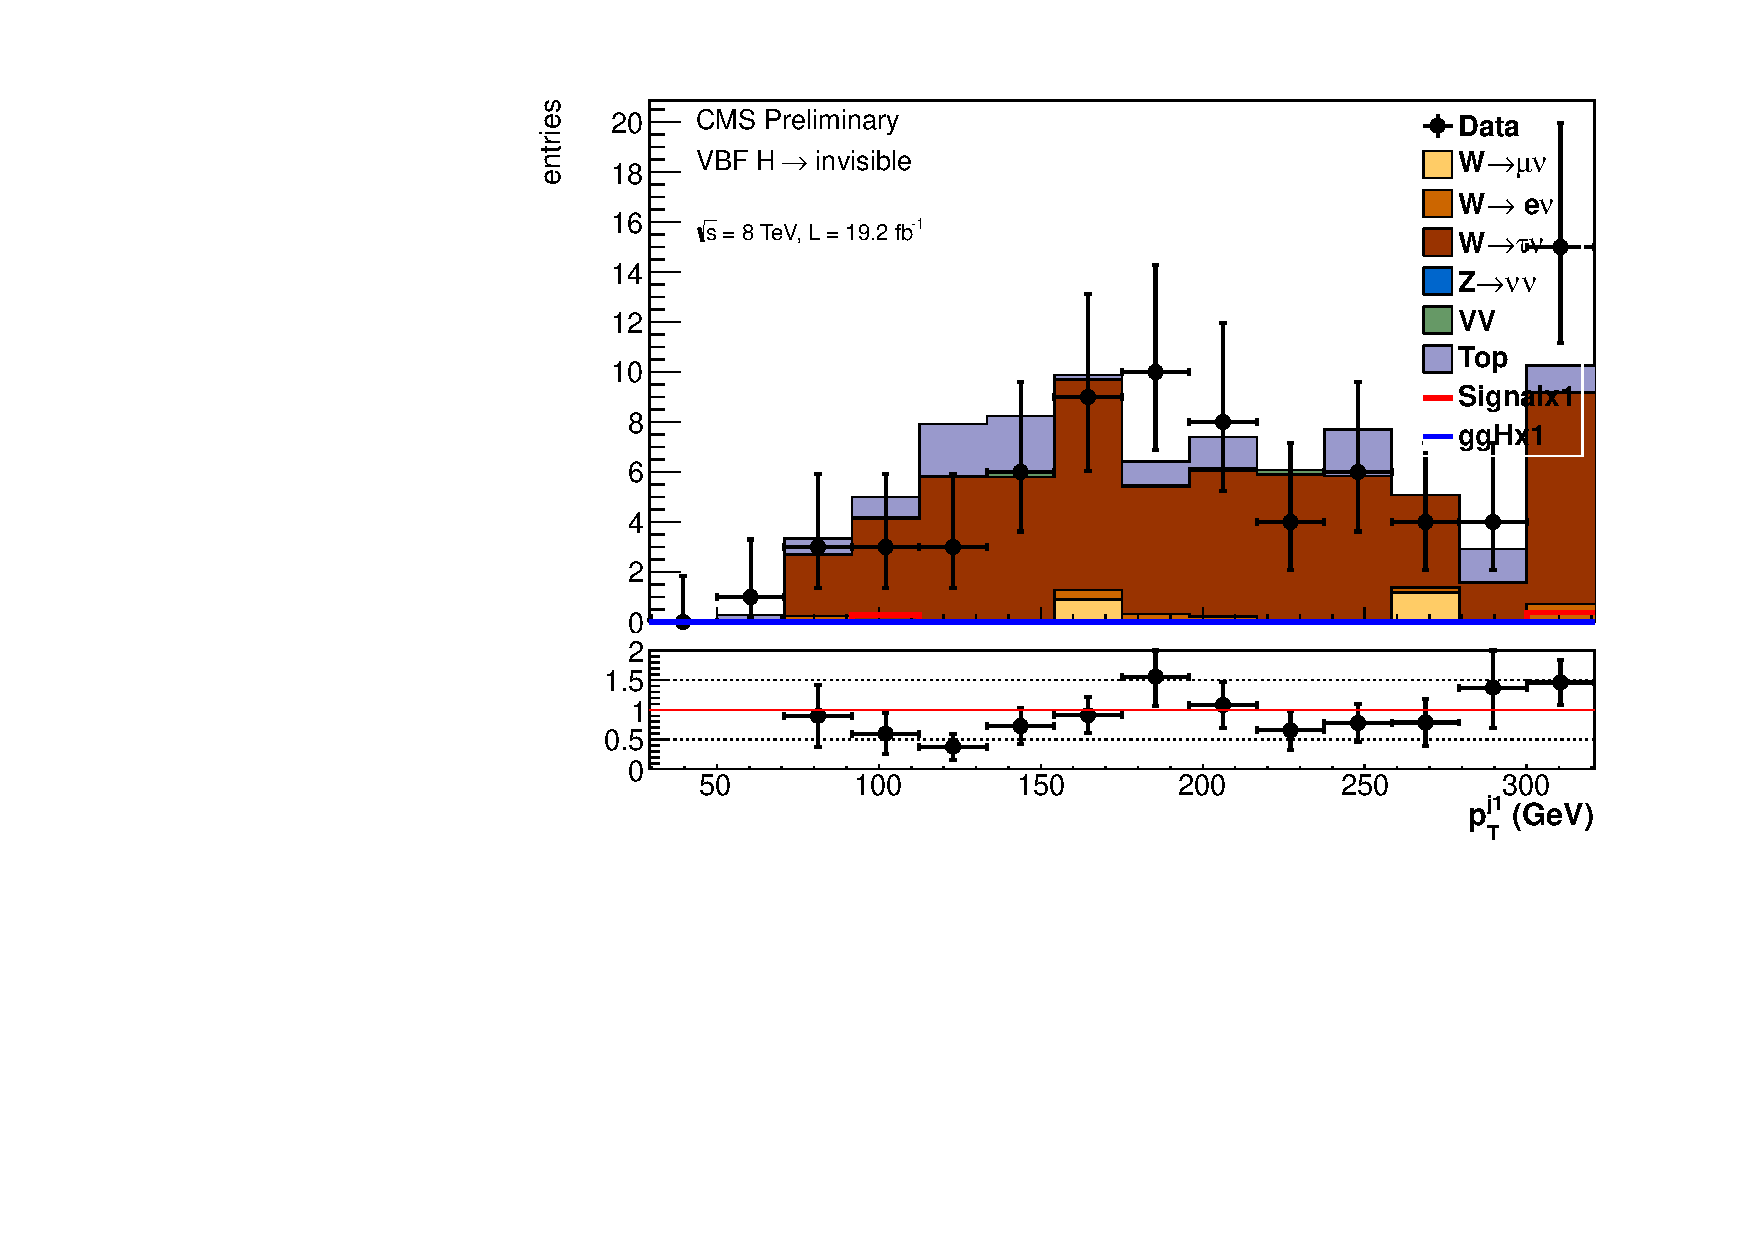
\includegraphics[width=.55\largefigwidth]{plots/parked/AN-14-243-figs/output_sigreg/taunu_jet1_pt.pdf}}
  \subfloat[]{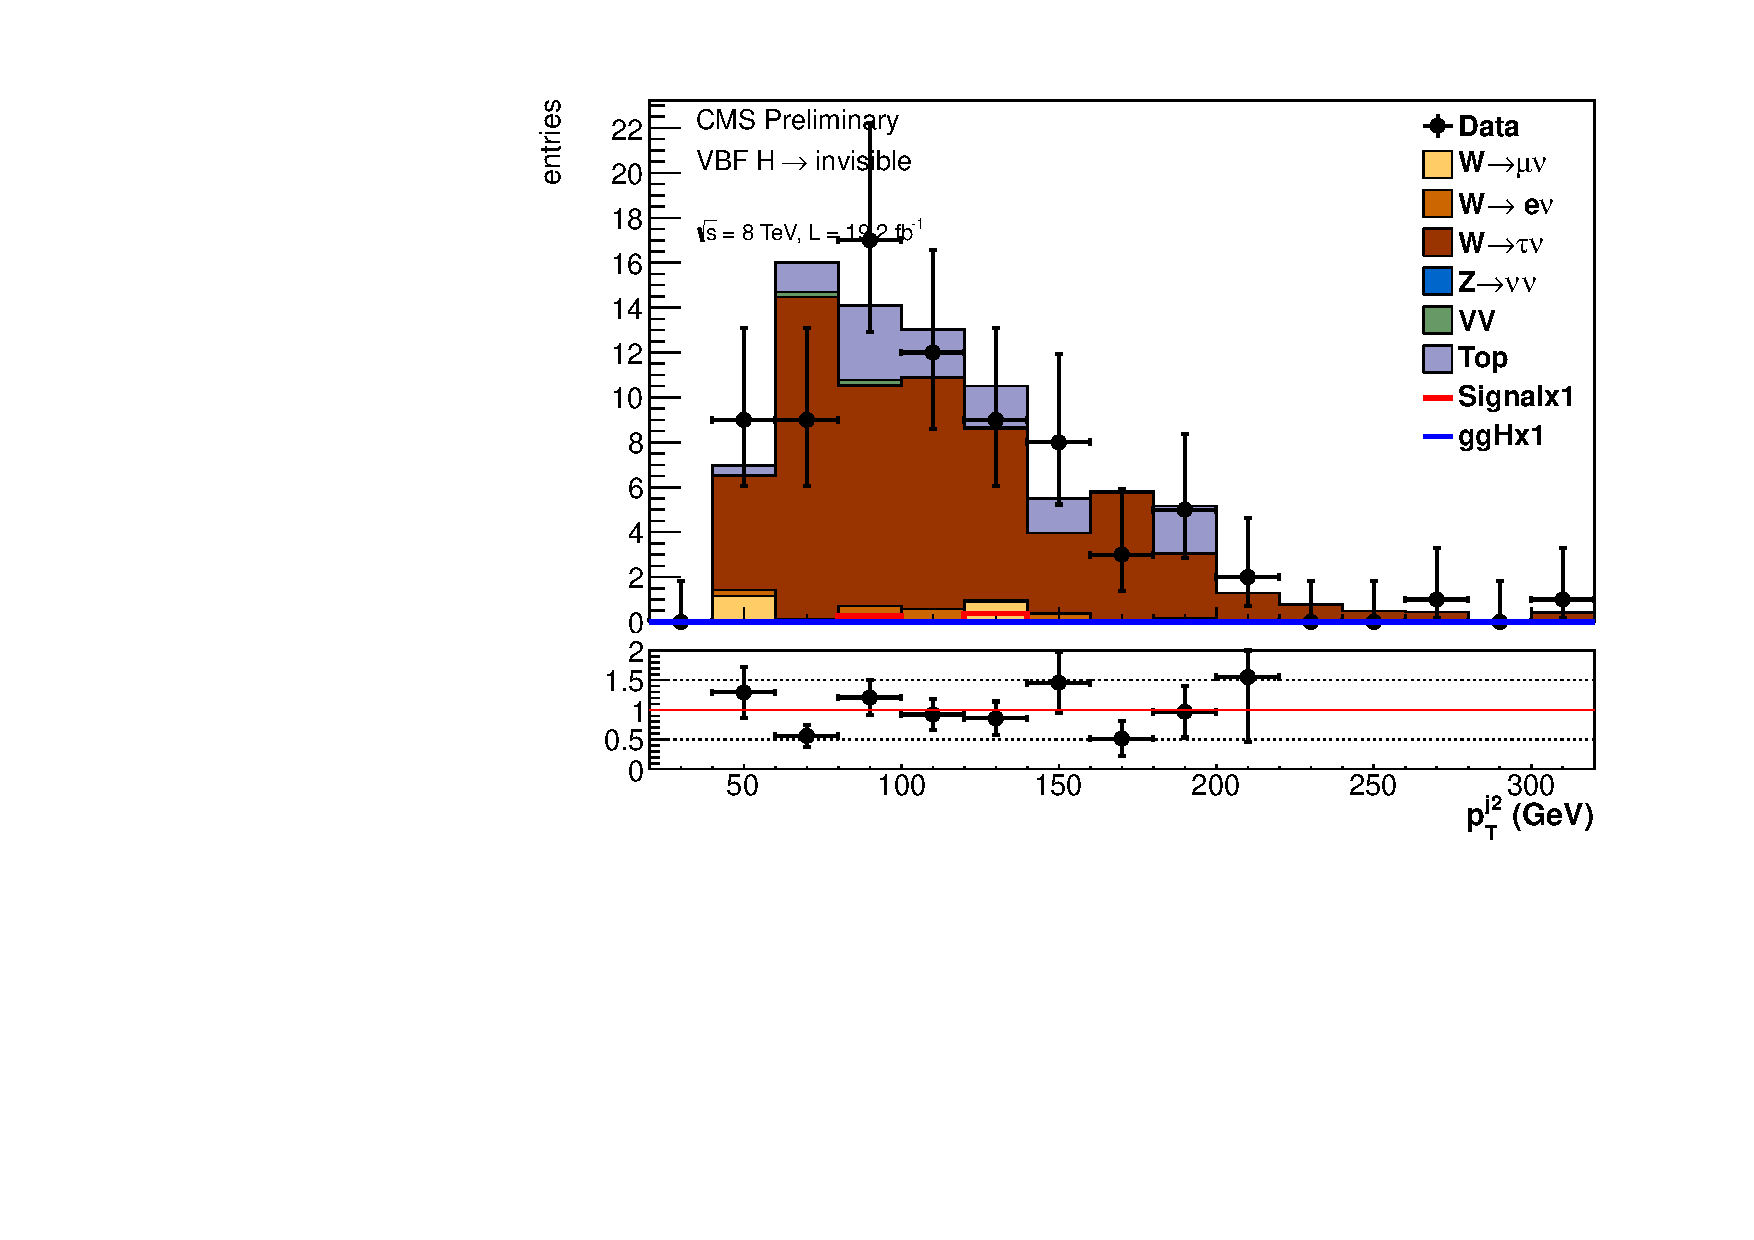
\includegraphics[width=.55\largefigwidth]{plots/parked/AN-14-243-figs/output_sigreg/taunu_jet2_pt.pdf}}

  \subfloat[]{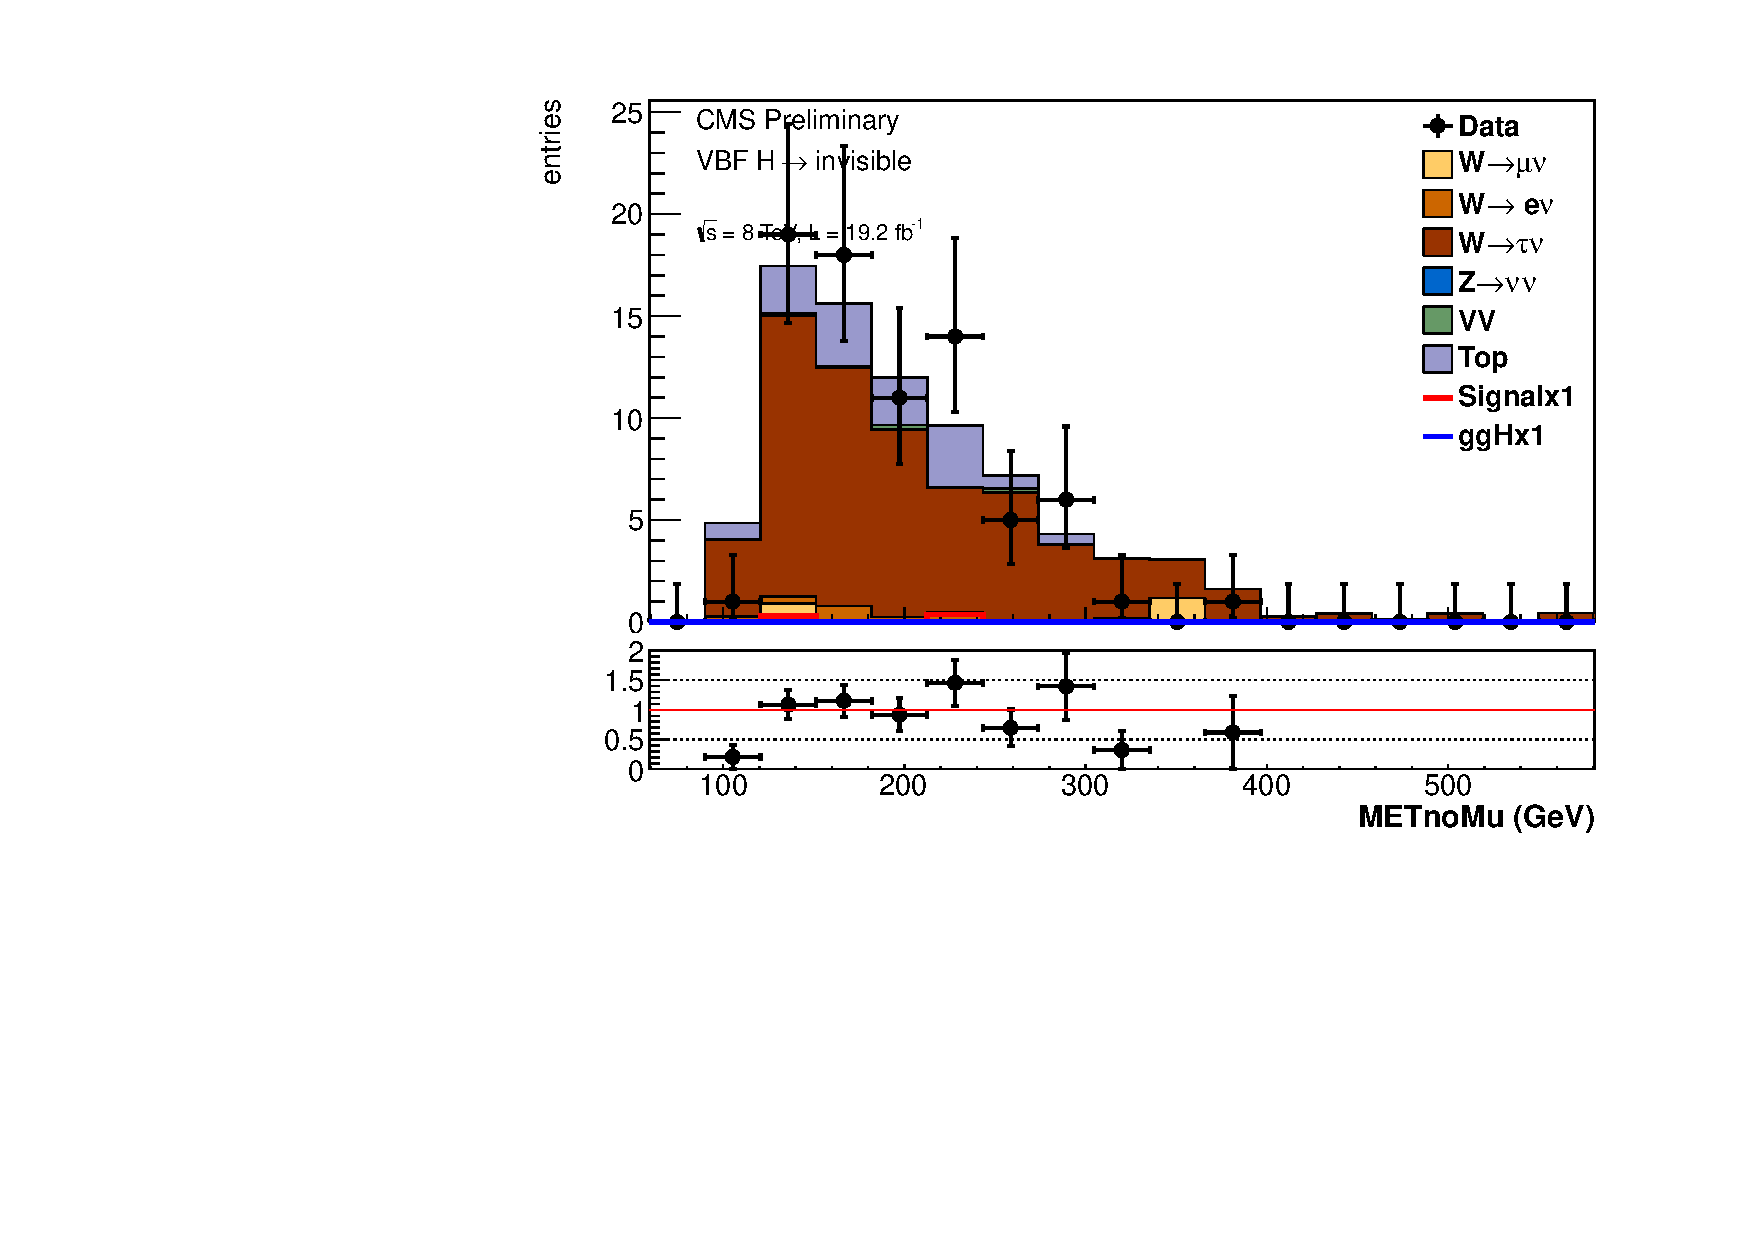
\includegraphics[width=.55\largefigwidth]{plots/parked/AN-14-243-figs/output_sigreg/taunu_metnomuons.pdf}}
  \subfloat[]{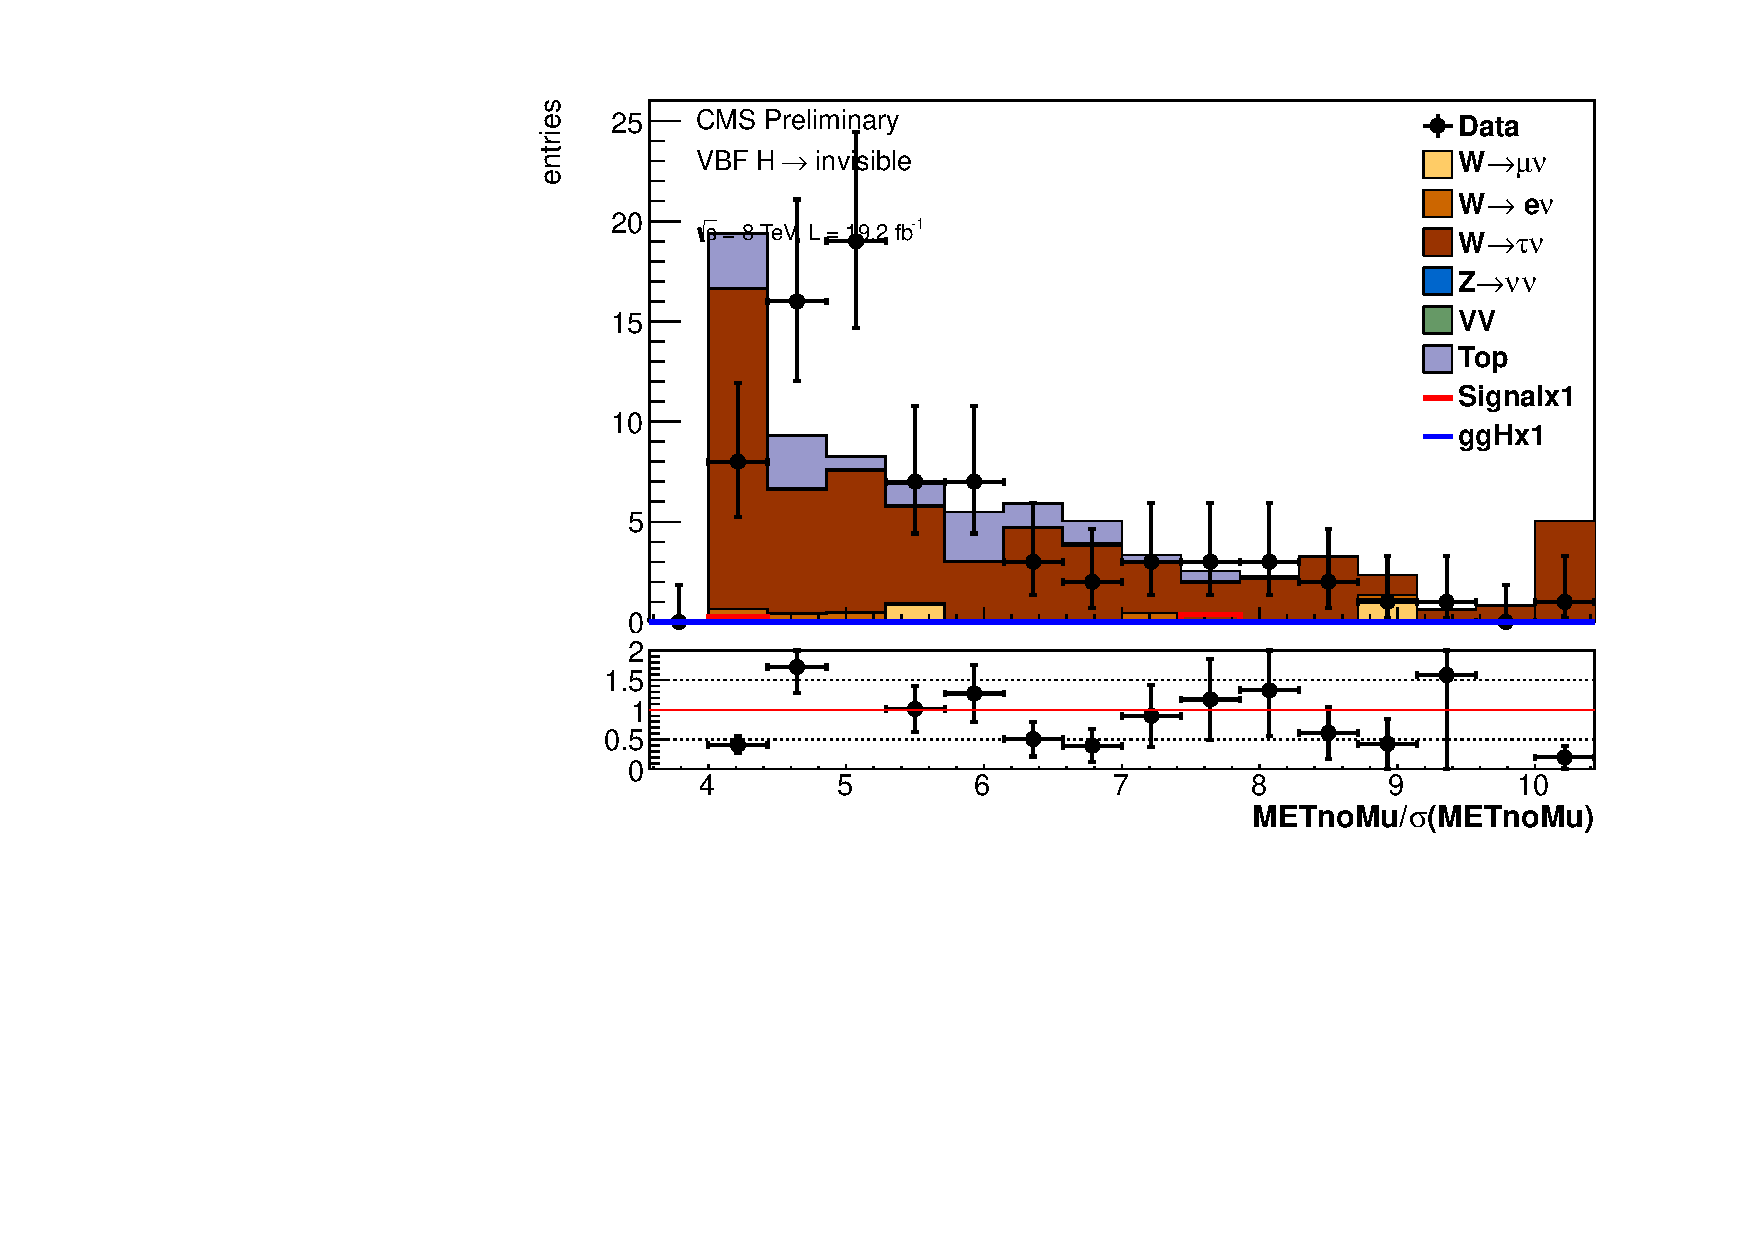
\includegraphics[width=.55\largefigwidth]{plots/parked/AN-14-243-figs/output_sigreg/taunu_metnomu_significance.pdf}}

  \subfloat[]{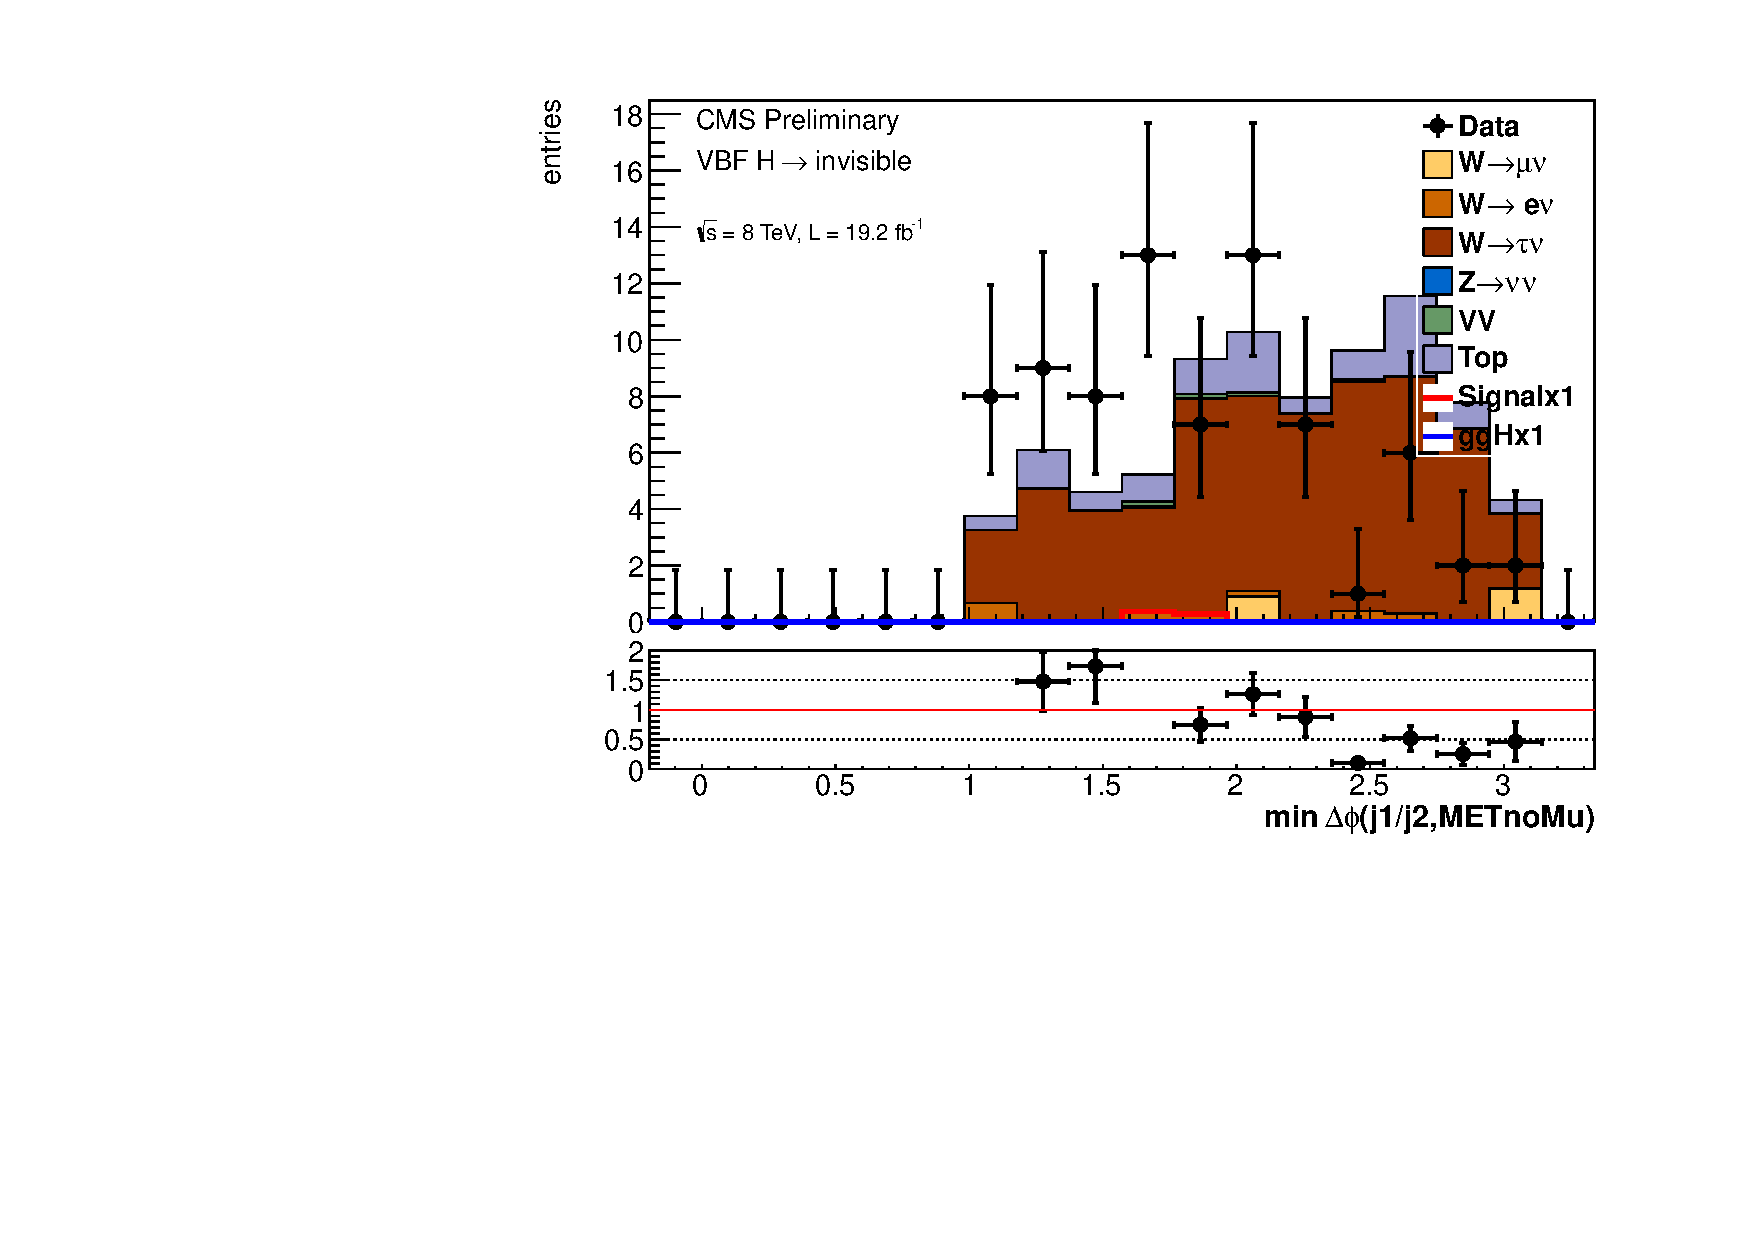
\includegraphics[width=.55\largefigwidth]{plots/parked/AN-14-243-figs/output_sigreg/taunu_jetmetnomu_mindphi.pdf}}
  \subfloat[]{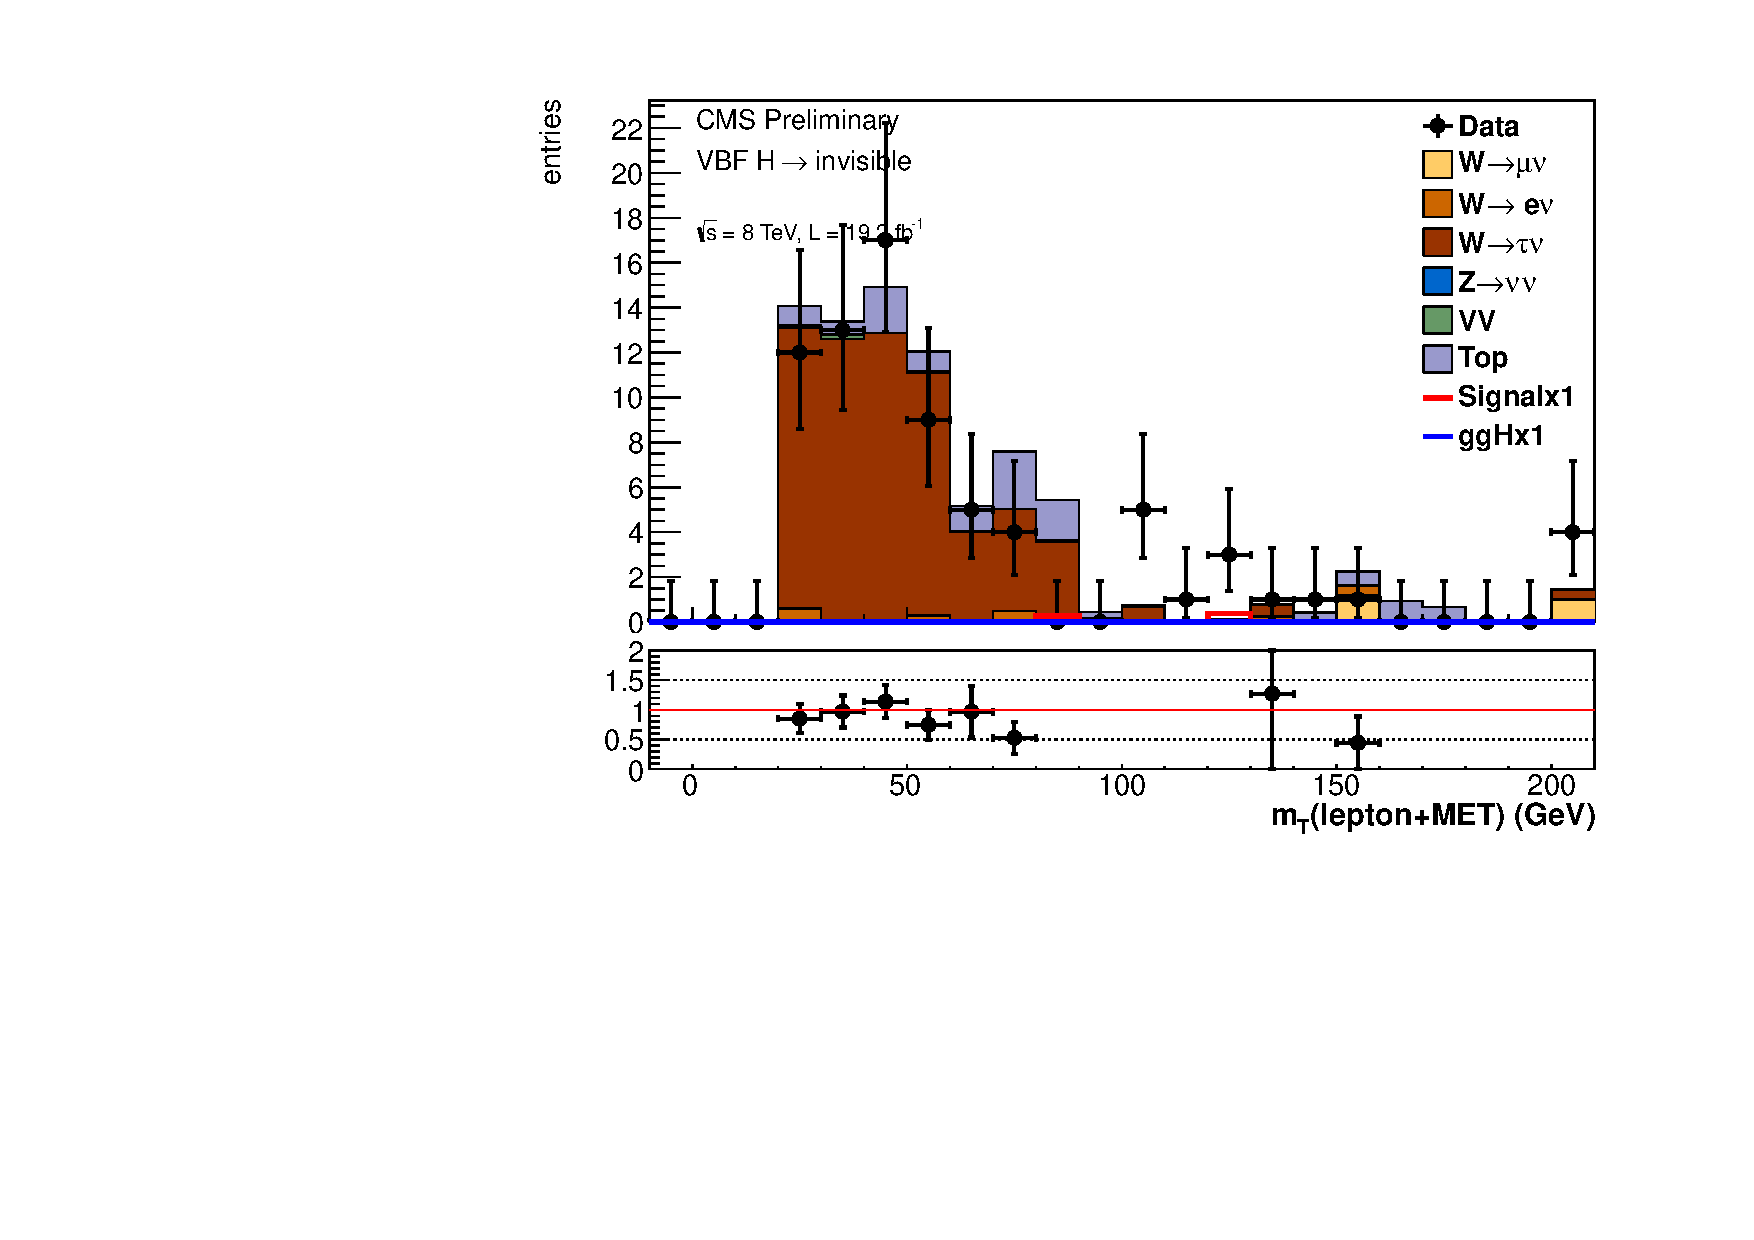
\includegraphics[width=.55\largefigwidth]{plots/parked/AN-14-243-figs/output_sigreg/taunu_lep_mt.pdf}}
  \caption{Distributions of variables in data and \ac{MC} events in the $\PW\rightarrow e\nu$ control region. \ac{MC} events from V+jets backgrounds are scaled by their data-driven scale factors. The variables shown are from top to bottom and left to right \detajj, \Mjj, the leading and subleading jet's \pt, \METnoMU, \METsig, \jetmetdphileading and the tau-\MET system's transverse mass.}
  \label{fig:parkedwtaunu}
\end{figure}

\begin{table}[h!]
  \begin{center}
    \caption{The inputs to and results of \EquationRef{eq:wdatabkgrep}, when used to estimate the $W\rightarrow \tau\nu$ estimate in the signal
      region.}
    \label{tab:parkedwtaunu}
    \begin{tabular}{lcc}
      \hline
      \hline
      & Signal region & Control region \\
      \hline
      \hline
      $N_{Data}$&N/A&$76\pm 8.7$\stat\\
      $N_{Bkg}$&N/A&$13.3\pm 2.8(MC stat)$\\
      $N_{MC}$&$121.9\pm 8.7(MC stat)$&$80.8\pm 6.4(MC stat)$\\
      \hline
      $\frac{N^{data}-N^{bkg}}{N^{MC}_{C}}$ & \multicolumn{2}{c|}{$0.78\pm 0.11$\stat$\pm 0.07$(MC stat.)} \\
      \hline
      $N_{\PW\rightarrow\mu\nu}$&\textcolor{red}{$94.6\pm 13.1$\stat$\pm 23.8$\syst}&N/A \\
      \hline
      \hline
    \end{tabular}
  \end{center}
\end{table}



\subsection{Differences between the $W\rightarrow e\nu$, $W\rightarrow\mu\nu$ and $W\rightarrow\tau\nu$ +jets backgrounds}
\label{sec:parkedenumunudiff}
%tau easily explainable by id eff
%sf for enu and munu different but compatible MC yield is where main difference is separate into into and out of acceptance and why (electrons in HF are jets, electron ID eff slightly worse) mindphijetmet shape difference outside acceptance
The number of \PW+jets events decaying to a particular flavour of lepton with \ac{VBF}-like jet kinematics should be the same for all three flavours of lepton through lepton universality~\cite{pdg}.
Differences between the numbers of background events from $\PW\rightarrow e\nu$ and $\PW\rightarrow \mu\nu$ and $\PW\rightarrow \tau\nu$ must therefore be due to differences in the identification of the leptons. Hadronic taus have much lower identification efficiencies than the other two flavours of leptons, so might naively be expected to give rise to a much larger number of background events. However, due to the similarities between hadronic taus and jets, unidentified taus often lead to additional jets in the event and therefore increase the probability that an event will fail the analysis \jetmetdphi cut~\cite{CMS-PAS-TAU-11-001}. These two competing effects mean that the number of background events from $\PW\rightarrow\tau\nu$ passing the signal region selection are not necessarily expected to be the same as those from $\PW\rightarrow e\nu$ and $\PW\rightarrow\mu\nu$.

By contrast, electrons and muons have much more similar identification efficiencies to each other (see Sections~\ref{sec:electrons} and \ref{sec:muons}). The 45\% difference in the number of expected background events from these two processes was therefore unexpected. This difference was also not seen in the prompt data analysis, as can be seen from \TableRef{tab:promptresults}. The prediction of the $\PW\rightarrow e/\mu\nu$ backgrounds is made up of a data driven scale factor and an estimate from \ac{MC} of the number of events from the process expected in the signal region, $N_{MC}^{S}$. Both these elements were studied to try to understand the observed differences.

Firstly, the data driven scale factors for the electron and muon backgrounds differ by 30\%, which is not sufficient to explain the full difference between the electron and muon background estimates. Furthermore, when systematic errors are taken into account this difference is only approximately one standard deviation. On the other hand, $N_{MC}^{S}$ does show a significant difference.

To study the difference in $N_{MC}^{S}$ two subregions of the signal region were studied, that with a generator level lepton inside the detector acceptance for both electrons and muons ($|\eta<2.1$), and that with a generator lepton outside the detector acceptance for both electrons and muons ($|\eta|>2.4$). The number of events in these two subregions from both $\PW\rightarrow e\nu$ and $\PW\rightarrow\mu\nu$ \ac{MC} can be seen in \TableRef{tab:enumunudiff}. The numbers of events with a generator level lepton inside acceptance are slightly but not much higher for electrons. This small difference is expected due to the lower identification efficiency for veto leptons making them less likely to cause an event to fail the lepton veto. Distributions of several variables were also studied for the inside acceptance events and found to be very similar for both $\PW\rightarrow e\nu$ and $\PW\rightarrow\mu\nu$ events.

Outside acceptance there are a lot more muon events than electron events. In this region neither flavour of lepton can be reconstructed and therefore cannot lead to an event failing the lepton veto, which implies that any difference is due to one or both flavours of lepton being reconstructed as a different object and affecting the jet or \MET related variables in the signal region selection. To study this effect further the \jetmetdphi requirement was relaxed to 1 and the distributions of several variables plotted for outside acceptance electron and muon events. Three of these distributions are shown in \FigureRef{fig:enumunudiff}. It can be seen from \FigureRef{fig:enumunudiff}a that electron events generally have more events than muon events. \FigureRef{fig:enumunudiff}b indicates that the electron events also have much lower values of \jetmetdphi. Finally, \FigureRef{fig:enumunudiff}c shows that there are very few events passing this region's selection requirements which have a generator level electron with \pt$>30$ \GeV, the threshold for jets to be included in the \jetmetdphi cut. These three pieces of information suggest that electrons are being reconstructed as jets when outside acceptance significantly more often than muons are. These misreconstructed jets then cause the electron events to fail the \jetmetdphi requirement.

It is to be expected that electrons outside of the detector acceptance will be reconstructed as jets, as these electrons will only be seen as deposits in the forward \ac{HCAL} and therefore be indistinguishable from jets. By contrast, muons deposit very little energy in the calorimetry systems, so will simply not be identified if they are outside of the muon system acceptance. No requirements were made on jets which were further forward in $\eta$ than the tag jets in the prompt data analysis, explaining why the difference in numbers of $\PW\rightarrow e\nu$ and $\PW\rightarrow\mu\nu$ events were not seen there.

\begin{table}
  \caption{The numbers of events predicted by \ac{MC} in the two subregions of the signal region with a generator level lepton that is inside/outside the detector acceptance for both electrons and muons from $\PW\rightarrow e\nu$ and $\PW\rightarrow\mu\nu$ processes. The errors shown are from \ac{MC} statistics.}
  \label{tab:enumunudiff}
  \begin{tabular}{lcc}
    \hline
    \hline
    Process & Inside acceptance & Outside acceptance \\
    \hline
    $\PW\rightarrow e\nu$ & $73.7\pm 6.8$ & $30.2\pm 4.9$ \\
    $\PW\rightarrow \mu\nu$ & $61.5\pm 6.8$ & $74.4\pm7.3$ \\
    \hline
    \hline
  \end{tabular}
\end{table}

\begin{figure}
  \subfloat[]{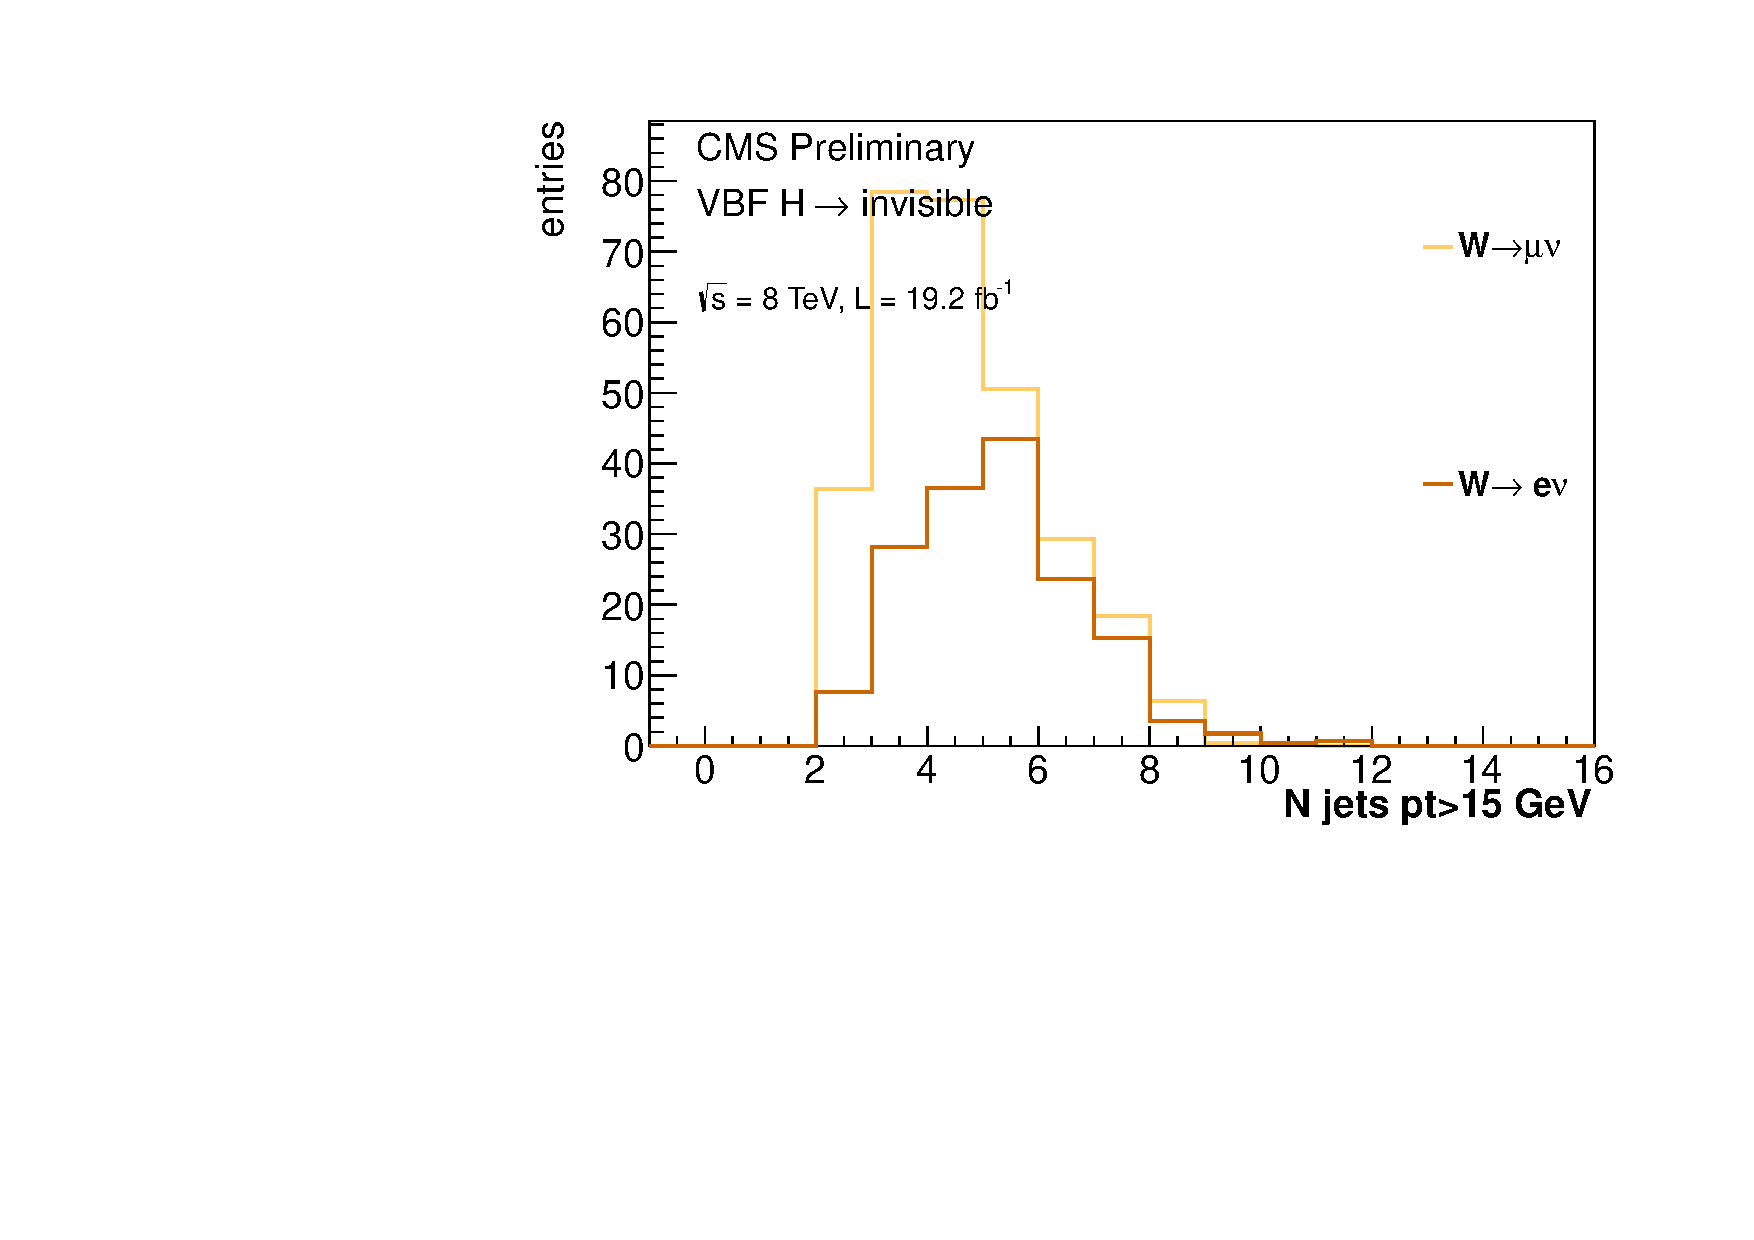
\includegraphics[width=.55\largefigwidth]{plots/parked/AN-14-243-figs/genlepstudy/outsideaccloosedphi/nunu_n_jets_15.pdf}}
  \subfloat[]{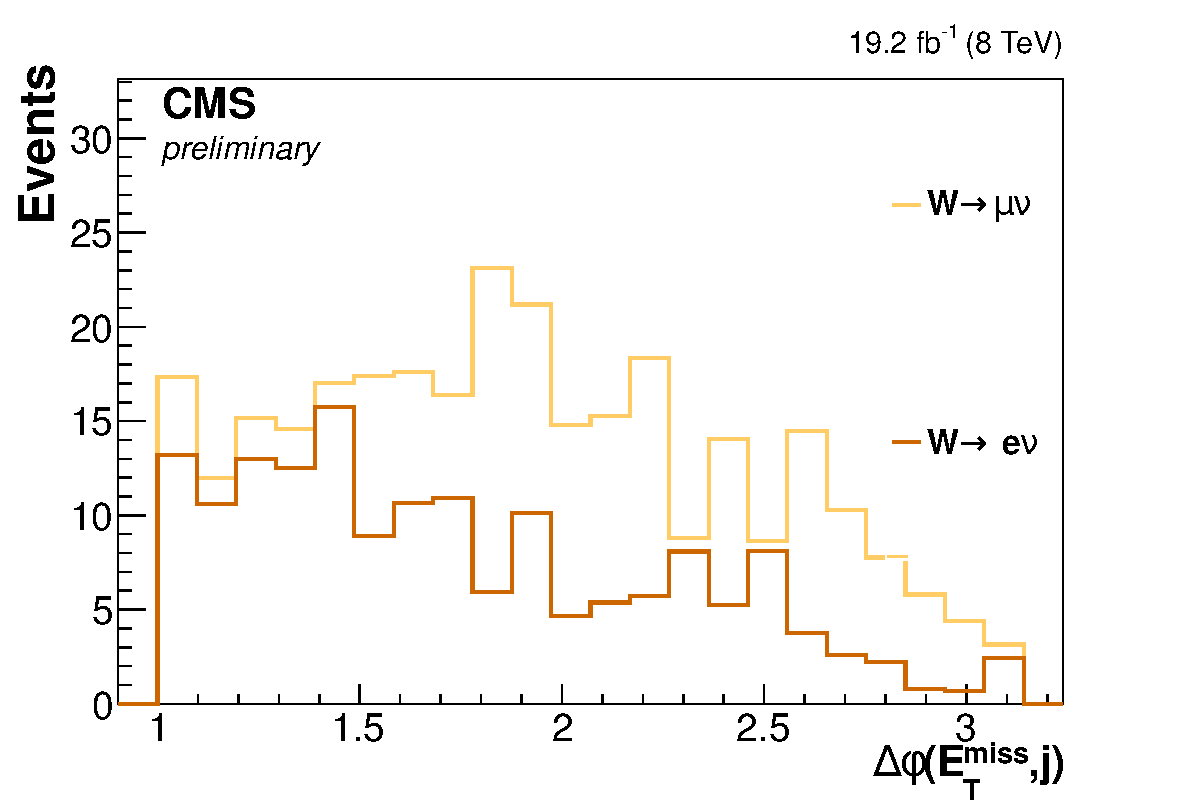
\includegraphics[width=.55\largefigwidth]{plots/parked/AN-14-243-figs/genlepstudy/outsideaccloosedphi/nunu_alljetsmetnomu_mindphi.pdf}}

  \subfloat[]{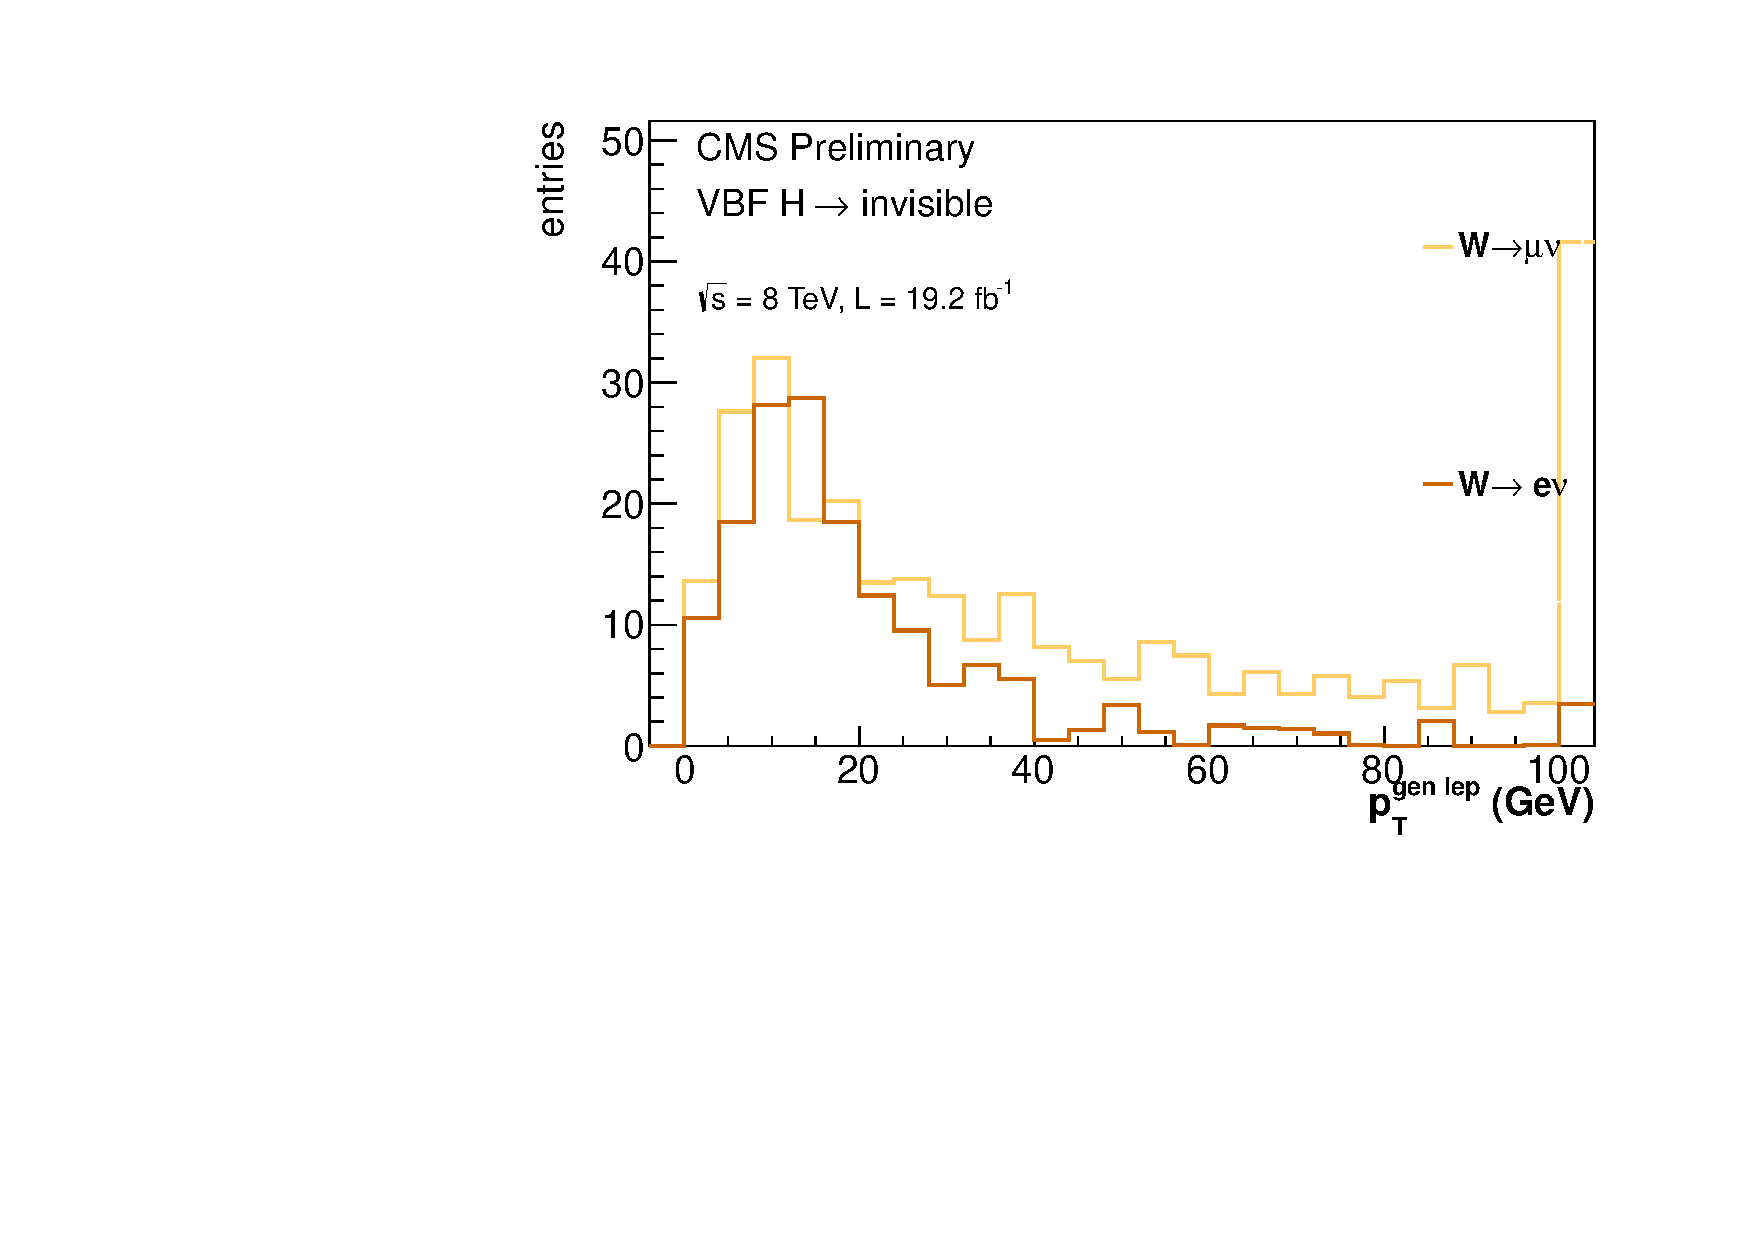
\includegraphics[width=.55\largefigwidth]{plots/parked/AN-14-243-figs/genlepstudy/outsideaccloosedphi/nunu_genlep1_pt.pdf}}
  \caption{Distributions of the number of jets with \pt$>15$ \GeV (a), \jetmetdphi (b) and the \pt of the leading generator level electron/muon in $\PW\rightarrow e/\mu\nu$ events in a region with cuts which are the same as those of the signal region except that the \jetmetdphi requirement has been loosened to 1 and a generator level lepton outside the detector acceptance for both electrons and muons is required.}
  \label{fig:enumunudiff}
\end{figure}

\subsection{Z$\rightarrow \nu\nu$+jets}%??                                                                                                                  
\label{sec:parkedznunu}
%??same as before studies of uncertainty with madgraph and mcfm
The irreducible $\PZ\rightarrow\nu\nu$ background is estimated using a very similar method to that used in the prompt data analysis, and a detailed description can be found in \SectionRef{sec:promptznunu}. A reminder of the method highlighting the differences from the prompt analysis is given here.

The method starts by defining a dimuon control region by taking the signal region requirements and replacing the muon veto with the requirement that there are two tight muons with invariant mass compatible with a \PZ boson, i.e. between 60 and 120 \GeV, and no other muons in the event. The number of events in this dimuon control region is then extrapolated to the signal region using efficiencies and cross-section ratios calculated using \ac{MC} events. As in the prompt data analysis \Zmumu \ac{MC} with the leptons removed and a requirement that there is a generator level dimuon system with invariant mass between 60 and 120 \GeV (i.e. compatible with a \PZ boson) is used to estimate the contribution in the signal region from \Znunu processes. \Znunu \ac{MC} events are not used for this estimation due to the limited size of the available \Znunu \ac{MC} samples. 

The formulas used to carry out the extrapolation from the control region to the signal region are given in Equations~\ref{eq:zdatabkg}, \ref{eq:zdataeffs} and \ref{eq:zdataeffc} which are repeated here for reference:
\begin{equation}
  \label{eq:zdatabkgrep}
  N^{S}_{Exp}=N^{C}_{Data}-N^{C}_{Bkg}\cdot\frac{\sigma\left(\PZ\rightarrow\nu\nu\right)}{\sigma\left(\PZ/\gamma^{*}\rightarrow\mu\mu\right)}\cdot\frac{\epsilon^{S}_{VBF}}{\epsilon^{C}_{VBF}},
\end{equation}
where $\epsilon^{S}$ and $\epsilon^{C}$ are calculated as follows.
\begin{align}
  \label{eq:zdataeffsrep}
  \epsilon^{S}_{VBF}&=\frac{ \sigma\left(\PZ\rightarrow\nu\nu,EWK\right) \frac{N^{S}_{MC}\left(EWK\right)} {N_{gen}\left(\PZ \rm{mass},EWK\right)} + \sigma\left(\PZ\rightarrow\nu\nu,QCD\right) \frac{N^{S}_{MC}\left(QCD\right)} {N_{gen}\left(\PZ \rm{mass},QCD\right)} } {\sigma\left(\PZ\rightarrow\nu\nu,EWK\right) + \sigma\left(\PZ\rightarrow\nu\nu,QCD\right)},\\
  \label{eq:zdataeffcrep}
  \epsilon^{C}_{VBF}&=\frac{  \sigma\left(\PZ/\gamma^{*}\rightarrow\mu\mu,EWK\right) \frac{N^{C}_{MC}\left(EWK\right)} {N_{gen}\left(EWK\right)} + \sigma\left(\PZ/\gamma^{*}\rightarrow\mu\mu,QCD\right) \frac{N^{S}_{MC}\left(QCD\right)} {N_{gen}\left(QCD\right)}  }{\sigma\left(\PZ/\gamma^{*}\rightarrow\mu\mu,EWK\right)+\sigma\left(\PZ/\gamma^{*}\rightarrow\mu\mu,QCD\right)},
\end{align}

%??inputs where the same and where different from prompt
%??studies of uncertainty on cross-section ratio

\subsection{V+jets closure tests}%??
\label{sec:parkedclosure}
%??as in AN relatively good agreement but large uncertainties

\subsection{V+jets scale factor investigations}%??
\label{sec:parkedscalefactors}
%??as in AN

\subsection{QCD}%??                                                                                                                                         
\label{sec:parkedQCD}
%??as in AN use isolated non-isolated met analogy with other methods
%??justify as high unc estimation of small background not perfect method


\subsection{Minor backgrounds}%??
\label{sec:parkedminor}
%??straight from MC same XSec measurements as prompt

\section{Systematic uncertainties}%??
\label{sec:parkedsyst}
The uncertainty due to the reweighting process used to account for trigger inefficiencies cancels in all data driven background estimates, as a ratio of \ac{MC} event yields is taken. To estimate the size of the uncertainty that should be applied to processes not taken from data driven background, the bin with the largest uncertainties on its fit for each era was chosen. It was then assumed that all bins had this worst-case uncertainty. This resulted in a 2.3\% overall uncertainty on these processes from this effect. Given that this error is smaller than many of the other errors considered, and that the uncertainty on the efficiency in most of the fit bins is significantly lower than this worst case this uncertainty is considered negligible.

%??explain uncertainty impact calculations and pulls test and give order of importance of nuisances state no issues found with pulls.

\section{Results}%??                                                                                                                                        
\label{sec:parkedresults}
%??cont plots
%??limit brazil plots
%??likelihood scans
